%%%---PREAMBLE---%%%%%%%%%%%%%%%%%%%%%%%%%%%%
\documentclass[twoside,12pt,final]{ucthesis-CA2012}

% fix for pandoc 1.14
\providecommand{\tightlist}{%
  \setlength{\itemsep}{0pt}\setlength{\parskip}{0pt}}

%--- Packages ---------------------------------------------------------
\usepackage[lofdepth,lotdepth,caption=false]{subfig}
\usepackage{fancyhdr}
\usepackage{amsmath, amssymb, graphicx}
\usepackage{xspace}
\usepackage{braket}
\usepackage{color}
\usepackage{setspace}
\usepackage{fancyvrb}
\usepackage{array}
\usepackage{ifxetex,ifluatex}
\usepackage{etoolbox}
\usepackage[width=.95\textwidth]{caption}

%% for the per mil symbol
\usepackage[nointegrals]{wasysym}

% more attractive tables
\usepackage{booktabs}
\usepackage{xcolor}
\usepackage{tabu}
\usepackage{tabularx}
\usepackage{lscape}
\usepackage{longtable}
\usepackage{titlesec}
\usepackage{longtable}

\usepackage[nostamp]{draftwatermark}
% % Use the following to make modification
\SetWatermarkText{DRAFT}
\SetWatermarkLightness{0.95}

%---New Definitions and Commands------------------------------------------------------

\newtheorem{theorem}{Jibberish}

\bibliography{references}

\hyphenation{mar-gin-al-ia}

% from uw_template.tex

% commands and environments needed by pandoc snippets
% extracted from the output of `pandoc -s`
%% Make R markdown code chunks work

\ifxetex
  \usepackage{fontspec,xltxtra,xunicode}
  \defaultfontfeatures{Mapping=tex-text,Scale=MatchLowercase}
\else
  \ifluatex
    \usepackage{fontspec}
    \defaultfontfeatures{Mapping=tex-text,Scale=MatchLowercase}
  \else
    \usepackage[utf8]{inputenc}
  \fi
\fi
\DefineShortVerb[commandchars=\\\{\}]{\|}
\DefineVerbatimEnvironment{Highlighting}{Verbatim}{commandchars=\\\{\},',fontsize=\small' }
% Add ',fontsize=\small' for more characters per line
\newenvironment{Shaded}{}{}
\newcommand{\KeywordTok}[1]{\textcolor[rgb]{0.00,0.44,0.13}{\textbf{{#1}}}}
\newcommand{\DataTypeTok}[1]{\textcolor[rgb]{0.56,0.13,0.00}{{#1}}}
\newcommand{\DecValTok}[1]{\textcolor[rgb]{0.25,0.63,0.44}{{#1}}}
\newcommand{\BaseNTok}[1]{\textcolor[rgb]{0.25,0.63,0.44}{{#1}}}
\newcommand{\FloatTok}[1]{\textcolor[rgb]{0.25,0.63,0.44}{{#1}}}
\newcommand{\CharTok}[1]{\textcolor[rgb]{0.25,0.44,0.63}{{#1}}}
\newcommand{\StringTok}[1]{\textcolor[rgb]{0.25,0.44,0.63}{{#1}}}
\newcommand{\CommentTok}[1]{\textcolor[rgb]{0.38,0.63,0.69}{\textit{{#1}}}}
\newcommand{\OtherTok}[1]{\textcolor[rgb]{0.00,0.44,0.13}{{#1}}}
\newcommand{\AlertTok}[1]{\textcolor[rgb]{1.00,0.00,0.00}{\textbf{{#1}}}}
\newcommand{\FunctionTok}[1]{\textcolor[rgb]{0.02,0.16,0.49}{{#1}}}
\newcommand{\RegionMarkerTok}[1]{{#1}}
\newcommand{\ErrorTok}[1]{\textcolor[rgb]{1.00,0.00,0.00}{\textbf{{#1}}}}
\newcommand{\NormalTok}[1]{{#1}}
\newcommand{\OperatorTok}[1]{\textcolor[rgb]{0.00,0.44,0.13}{\textbf{{#1}}}}
\newcommand{\BuiltInTok}[1]{\textcolor[rgb]{0.00,0.44,0.13}{\textbf{{#1}}}}
\newcommand{\ControlFlowTok}[1]{\textcolor[rgb]{0.00,0.44,0.13}{\textbf{{#1}}}}

\ifxetex
  \usepackage[setpagesize=false, % page size defined by xetex
              unicode=false, % unicode breaks when used with xetex
              xetex,
              colorlinks=true,
              linkcolor=blue]{hyperref}
\else
  \usepackage[unicode=true,
              colorlinks=true,
              linkcolor=blue]{hyperref}
\fi
\hypersetup{breaklinks=true, pdfborder={0 0 0}}
\setlength{\parindent}{0pt}
\setlength{\parskip}{6pt plus 2pt minus 1pt}
\setlength{\emergencystretch}{3em}  % prevent overfull lines
\setcounter{secnumdepth}{0}

%---Set Margins ------------------------------------------------------
\setlength\oddsidemargin{0.25 in} \setlength\evensidemargin{0.25 in} \setlength\textwidth{6.25 in} \setlength\textheight{8.50 in}
\setlength\footskip{0.25 in} \setlength\topmargin{0 in} \setlength\headheight{0.25 in} \setlength\headsep{0.25 in}

%%%---DOCUMENT---%%%%%%%%%%%%%%%%%%%%%%%%%%%%
\begin{document}

%=== Preliminary Pages ============================================
\begin{ucfrontmatter}

  %%%%%%%%%%%%%%%%%%%%%%%%%%%
  % TITLE PAGE INFORMATION %  modified to meet UCDavis, R. Peek, 2018
  %%%%%%%%%%%%%%%%%%%%%%%%%%%

  \title{The Diversity and Composition of Grassland Ecosystems Under Global Change}
  \author{Evan E. Batzer}

\report{DISSERTATION} 
  \degree{DOCTOR OF PHILOSOPHY} 
  \degreemonth{October} \degreeyear{2020}
  \chair{Valerie Eviner}  % this is your advisor
  \othermemberA{Susan Harrison} % This is a member of your committee
  \othermemberB{Andrew Latimer} % This is a member of your committee
  \othermemberC{} % This is a member of your committee
  \numberofmembers{3} % should match the number of entries above (chair + othermembers)
  \field{ECOLOGY}
  \campus{DAVIS}
  
	\maketitle
	
	% APPROVAL AND COPYRIGHT
	% \approvalpage % AS OF 2018 Fall, don't need this additional page if use cover page for signatures
	% \copyrightpage
  
  % ACKNOWLEDGEMENTS
\begin{acknowledgements}
    ``Thank you to everyone''
  \end{acknowledgements}
  %%%%%%
  % CV % Not required, add if you need
  %%%%%%
%   \begin{vitae}
%     \addcontentsline{toc}{chapter}{Curriculum Vitae}
% 
%     \begin{vitaesection}{Education}
%     \vspace{-0.1cm}
%     \item [2018]	Ph.D. in Environmental Science and Management (Expected), University of California, Santa Barbara.
%     \item [2010]	MESM in in Environmental Science and Management, University of California, Santa Barbara.
%     \item [2007]	B.S. in Ecosystem Science and Policy and Biology, University of Miami
%     \end{vitaesection}
% 
%     \textbf{Publications}
% 
%     Anderson, S.C., Cooper, A.B., Jensen, O.P., Minto, C., Thorson, J.T., Walsh, J.C., Afflerbach, J., Dickey‐Collas, M., Kleisner, K.M., Longo, C., Osio, G.C., Ovando, D., Mosqueira, I., Rosenberg, A.A., Selig, E.R., n.d. Improving estimates of population status and trend with superensemble models. Fish and Fisheries 18, 732–741. https://doi.org/10.1111/faf.12200
% 
%  Burgess, M.G., McDermott, G.R., Owashi, B., Reeves, L.E.P., Clavelle, T., Ovando, D., Wallace, B.P., Lewison, R.L., Gaines, S.D., Costello, C., 2018. Protecting marine mammals, turtles, and birds by rebuilding global fisheries. Science 359, 1255–1258. https://doi.org/10.1126/science.aao4248
% 
% Costello, C., Ovando, D., Clavelle, T., Strauss, C.K., Hilborn, R., Melnychuk, M.C., Branch, T.A., Gaines, S.D., Szuwalski, C.S., Cabral, R.B., Rader, D.N., Leland, A., 2016. Global fishery prospects under contrasting management regimes. PNAS 113, 5125–5129. https://doi.org/10.1073/pnas.1520420113
% 
% \end{vitae}

	%%%%%%%%%%%%%%%%%%%%%%%%%%%
  % ABSTRACT %
  %%%%%%%%%%%%%%%%%%%%%%%%%%%
  \begin{abstract}
    \addcontentsline{toc}{chapter}{Abstract}

    ""

    %\abstractsignature
  \end{abstract}
  % TABLE OF CONTENTS
	\tableofcontents

	  \listoftables
  
    \listoffigures
  
\end{ucfrontmatter}
\begin{ucmainmatter}

\hypertarget{the-neutral-theory-of-niche-dimensionality}{%
\chapter{The ``Neutral Theory'' of Niche Dimensionality}\label{the-neutral-theory-of-niche-dimensionality}}

\chaptermark{Response dimensionality}

Evan E. Batzer\textsuperscript{1*},
Siddharth Bharath\textsuperscript{2},
Elizabeth Borer\textsuperscript{2},
Stan Harpole\textsuperscript{3},
Carlos Alberto Arnillas\textsuperscript{4},
Miguel Bugalho\textsuperscript{5},
Maria Caldeira\textsuperscript{6},
Oliver Carroll\textsuperscript{7},
Mick Crawley\textsuperscript{8},
Kendi Davies\textsuperscript{9},
Pedro Daleo\textsuperscript{10},
Johannes Knops\textsuperscript{11},
Kimberly Komatsu\textsuperscript{12},
Andrew MacDougall\textsuperscript{7},
Rebecca L. McCulley\textsuperscript{13},
Brett Melbourne\textsuperscript{9},
Timothy Ohlert\textsuperscript{14},
Sally A. Power\textsuperscript{15},
Suzanne Prober\textsuperscript{16},
Christiane Roscher\textsuperscript{3,17},
Mahesh Sankaran\textsuperscript{18,19},
Glenda Wardle\textsuperscript{20},
George Wheeler\textsuperscript{21},
Peter Wilfhart\textsuperscript{2},
and Eric Seabloom\textsuperscript{2}.
\begin{enumerate}
\def\labelenumi{\arabic{enumi}.}
\tightlist
\item
  Department of Plant Sciences, University of California, Davis, USA
\item
  Department of Ecology, Evolution, and Behavior, University of Minnesota, USA
\item
  Department for Physiological Diversity, German Centre for Integrative Biodiversity Research (iDiv), Germany
\item
  University of Toronto at Scarborough, Canada
\item
  Centre for Applied Ecology (CEABN-InBIO), University of Lisbon, Portugal
\item
  Forest Research Centre, School of Agriculture, University of Lisbon, Portugal
\item
  Imperial College London, Silwood Park, UK
\item
  University of Guelph, Canada
\item
  Department of Ecology and Evolutionary Biology, University of Colorado, Boulder, USA
\item
  Instituto de Investigaciones Marinas y Costeras (IIMyC), CONICET -- UNMDP, Argentina
\item
  Department of Health \& Environmental Sciences, Xi'an Jiaotong Liverpool University, Suzhou, China
\item
  Smithsonian Environmental Research Center, Edgewater, USA
\item
  Department of Plant and Soil Sciences, University of Kentucky, Lexington, USA
\item
  Department of Biology, University of New Mexico
\item
  Hawkesbury Institute for the Environment, Western Sydney University, Australia
\item
  CSIRO Land and Water, Australia
\item
  UFZ, Helmholtz Centre for Environmental Research, Physiological Diversity, Germany
\item
  National Centre for Biological Sciences, TIFR, India
\item
  School of Biology, University of Leeds, UK
\item
  School of Life and Environmental Sciences, University of Sydney, Australia
\item
  School of Biological Sciences, University of Nebraska, Lincoln, USA
\end{enumerate}
\hypertarget{abstract}{%
\section{Abstract}\label{abstract}}

Increases in the availability of limiting soil nutrients are known to produce changes in plant community diversity and composition. Among locally interacting species, this change is tied to competitive trade-offs across gradients of resource availability. Plant responses to fertilization are often thought to be mediated through aboveground competition, where effective competitors are better able to intercept available light.
However, plant communities are often subject to simultaneous limitation by multiple nutrients, which may lead to multidimensional trade-offs in the use of individual belowground resources. Depending on the contributions of these two mechanisms to species interactions, treatment effects may vary in their dimensionality -- the degree to which community responses to fertilization can be captured across a single axis of change.
Using data from a globally replicated nutrient addition experiment, we assessed the dimensionality of community response to fertilization across three different resource addition treatments. Across all studies, species responses to nutrient enrichment were broadly consistent across multiple enrichment treatments, suggesting that fertilization often acts on a one-dimensional trade-off governed by light limitation.
However, we also found significant deviations from this general relationship across plant functional groups and local contexts; sites characterized by high pre-treatment productivity and legume abundance exhibited more variation in the direction of community change across treatments. Our findings suggest that while broad functional trade-offs may predominate at a global scale, community responses to fertilization are likely to depend on site-specific variation in coexistence mechanisms.

\hypertarget{introduction}{%
\section{Introduction}\label{introduction}}

Human alterations of the earth's biogeochemical cycles have produced widespread changes in the availability of key nutrients known to control plant productivity (Vitousek et al. \protect\hyperlink{ref-Vitousek1997b}{1997}, Elser et al. \protect\hyperlink{ref-Elser2007}{2007}).
Increased concentrations of soil nutrients are recognized as important drivers of compositional change in plant communities, resulting in altered patterns of abundance and diversity (Tilman \protect\hyperlink{ref-Tilman1984}{1984}, Tilman and Lehman \protect\hyperlink{ref-Tilman2001}{2001}).
In turn, these effects on community structure are implicated in changes to key ecosystem properties, including reductions in resilience, resistance, and loss of multifunctionality (Chapin et al. \protect\hyperlink{ref-Chapin2000}{2000}, Hector and Bagchi \protect\hyperlink{ref-Hector2007}{2007}, Isbell et al. \protect\hyperlink{ref-Isbell2015}{2015}).
Nutrient enrichment is thought to control plant community composition through environmental shifts that operate on niche differences among interacting species. Given that photosynthetic organisms compete for a similar set of limiting resources (Hutchinson 1961), plant coexistence is likely mediated by trade-offs in resource use that produce variable fitness across environments. It is through these trade-offs that nutrient enrichment drives changes in plant abundance, favoring species that are better able to exclude their competitors under elevated nutrient conditions (Tilman \protect\hyperlink{ref-Tilman1984}{1984}).
To effectively predict compositional shifts following nutrient enrichment, it is thus essential to identify the specific mechanisms that govern plant responses. In many cases, fertilization is linked to a shift between soil nutrients and light as the primary limiting factor for plant growth ({\textbf{???}}, Tilman \protect\hyperlink{ref-Tilman1984}{1984}, Dybzinski and Tilman \protect\hyperlink{ref-Dybzinski2007a}{2007}, Hautier et al. \protect\hyperlink{ref-Hautier2009}{2009}, Clark et al. \protect\hyperlink{ref-Clark2018}{2018}).
The increased abundance of taller species under elevated nutrient inputs suggests a one-dimensional trade-off where plants are differentiated by their ability to acquire belowground resources or intercept available light (Hautier et al. \protect\hyperlink{ref-Hautier2009}{2009}, DeMalach et al. \protect\hyperlink{ref-DeMalach2017a}{2017}).
However, fertilization effects may not be limited to a single driver. Plants are also known to be limited by (and compete for) multiple belowground resources, even in high productivity contexts (Wilson and Tilman \protect\hyperlink{ref-Wilson1991}{1991}, Fay et al. \protect\hyperlink{ref-Fay2015}{2015}, Harpole et al. \protect\hyperlink{ref-Harpole2016}{2016}).
As a result, biodiversity loss may also stem from multi-dimensional trade-offs in the use and acquisition of individual soil nutrients. In this perspective, plant responses to fertilization are governed by variation in species' ability to utilize specific soil resources, such nitrogen, phosphorous, potassium, or other micronutrients (Harpole and Tilman \protect\hyperlink{ref-Harpole2007}{2007}, Harpole et al. \protect\hyperlink{ref-Harpole2016}{2016}).
While trade-offs mediated by light competition or the use of individual soil resources explain declines in species richness following fertilization, there exist few tests of their relative contribution to observed effects (but see DeMalach and Kadmon (\protect\hyperlink{ref-DeMalach2017b}{2017}) and Harpole et al. (\protect\hyperlink{ref-Harpole2017}{2017})).
However, these mechanisms present distinct predictions related to the dimensionality of community change across different nutrient enrichment treatments. Under a one-dimensional trade-off mediated by light competition, the addition of any limiting belowground resource will shift species abundances across a single axis.
As a result, treatment effects will be directionally equivalent in response to the enrichment of different soil resources. Nutrient-specific trade-offs, however, predict that fertilization effects depend on resource identity, leading to high-dimensional (dissimilar) shifts in composition that vary as a function of the specific soil nutrient added.

Observed patterns of plant niche differentiation offer lines of evidence supporting predictions of both one-dimensional and multi-dimensional patterns of change. At a global scale, conserved patterns of tissue stoichiometry (Ågren \protect\hyperlink{ref-Agren2008}{2008}) and dominant axes of plant functional variation (Díaz et al. \protect\hyperlink{ref-Diaz2016}{2016}) suggest that one-dimensional trade-offs are likely to predominate -- plant growth strategies may be expected to confer increased fitness under elevated nutrient concentrations generally, rather than varying in response to specific fertilization treatments ({\textbf{???}}).
However, outcomes of plant competition are the result of relative differences in resource use among interacting species (Tilman \protect\hyperlink{ref-tilman1982resource}{1982}).
Depending on community context, variation in plant nutrient demands and functional strategies may drive resource-specific trade-offs.
Critically, performance under variable nutrient concentrations only forms a subset of the possible forms of niche differentiation in plant communities. Correlated patterns of variation in plant functional characteristics and abundance suggest several key ways in which niche differentiation commonly occurs ({\textbf{???}}).
Plants are theorized to exhibit trade-offs between competition and colonization (Tilman \protect\hyperlink{ref-Tilman1994}{1994}, Pacala and Rees \protect\hyperlink{ref-Pacala1998}{1998}), herbivore defense and growth (Mattson and Herms \protect\hyperlink{ref-Mattson1992}{1992}), and between leaf longevity and photosynthetic rate (Wright et al. \protect\hyperlink{ref-Wright2004}{2004}, Reich \protect\hyperlink{ref-Reich2014}{2014}).
Depending on the strength of these other mechanisms, constraints on plant function and physiology may limit the development of nutrient-specific trade-offs; varied responses to different nutrient enrichment treatments may be more common in systems where belowground resource competition acts as an important coexistence mechanism ({\textbf{???}}, Brauer et al. \protect\hyperlink{ref-Brauer2012}{2012}, Hautier et al. \protect\hyperlink{ref-Hautier2018}{2018}).
For example, multi-dimensional trade-offs may be limited in systems characterized by stressful environmental conditions or reduced functional diversity that limit specialization on specific soil resources (Suding et al. \protect\hyperlink{ref-Suding2005}{2005}, Dwyer and Laughlin \protect\hyperlink{ref-Dwyer2017}{2017}).
Evaluation of the direction of compositional response to nutrient enrichment, broadly and in site-specific contexts, may identify mechanisms responsible fertilization-driven biodiversity change.
Here, we use a globally distributed experiment manipulating the availability of belowground resources to determine if there are tradeoffs in species responses to multiple nutrients.
In a geometric approach, we compare observed community response dimensionality to a neutral expectation in which species exhibit proportionally identical responses to the enrichment of multiple soil nutrients.
Deviations from this neutral model provide a metric to quantify the importance of tradeoffs that may drive diversity changes in response to increased nutrient supply rates.

We hypothesize that community responses to fertilization will be less varied (more one-dimensional) in spatially or temporally heterogeneous systems and those of lower productivity, where specialization on individual soil nutrients is unlikely to form an important axis of niche differentiation. In contrast, we expect multi-dimensional tradeoffs in belowground resource use to be more important in in taxonomically diverse, productive, spatially homogenous environments. Quantification of these patterns forms a critical tool to infer how local coexistence mechanisms control community responses to global change and improve predictions of their effects.

\hypertarget{methods}{%
\section{Methods}\label{methods}}

\emph{Study Sites}

We examined 49 study sites that are part of the Nutrient Network, a cooperative, globally distributed experiment (Borer et al.~2014a). Nutrient Network study sites are constructed in a randomized block design, typically composed of 3 blocks divided into 5m x 5m plots. In each block, we selected four plots to be used in experimental analysis: control plots with no supplemental nutrient enrichment and plots subject to fertilization of either nitrogen (N), phosphorous (P), or potassium with other micronutrients (Kµ), yielding 12 -- 20 plots per site.

All nutrient enrichment treatments were applied at a rate of 10 g N, P, or K m-2 year-1 as time-release urea, triple-super-phosphate, and potassium sulfate, respectively. A micronutrient mix (17\% Fe, 12\% S , 6\% Ca, 3\% Mg, 2.5\% Mn, 1\% Zn, 1\% Cu, 0.1\% B, and 0.05\% Mo) supplied as part of the Kµ treatment occurred only during the first treatment year at a rate of 100g m-2 to avoid accumulation toxicity.
Because sites were initialized at different years and observed for different durations, we filtered our dataset to focus on sites with at least 5 years of treatment, a sufficient number of treatment years to have confidence in observed community responses. All sites used in this analysis also included a pre-treatment year (Median = 9.36, Min = 5, Max = 13), which was used to establish baseline community composition metrics used in structural equation modeling. A full list of sites and their characteristics is presented in Appendix 1.

\emph{Response Measurements}

In each 5m x 5m plot, a 1m x 1m subplot was designated for community observation. Observers evaluated community composition annually, visually estimating areal cover of all species to the nearest 1 percent. Cover for each species was estimated independently, yielding total cover values that often exceeded 100\% in vertically stratified communities. We focused our analysis on species with well-characterized responses to nutrient enrichment by including taxa that were observed in all treatments and present in at least 33\% of all community observations within a site. Our filtering criteria included species across a range of mean abundance, and in most sites, captured a large proportion of the total observed community cover in control plots (Median = 0.88, Min = 0.36, Max = 0.99).
To evaluate relationships between plant life history strategy and fertilization response, species were divided into four functional groups: graminoids (order Poales), legumes (family Fabaceae), woody species, and forbs. At each site, plants were also characterized by local longevity (annual / biennial / perennial) and provenance (native / introduced).

In most sites, photosynthetically active radiation (PAR) was measured using a ceptometer placed above the grassland canopy and at the soil surface. Light interception was estimated as the fraction of available PAR above the canopy relative to available PAR on the soil surface.

In a separate subplot, aboveground biomass was collected yearly in two 1m x 10cm strips of vegetation, air dried to a constant mass at 60º C, and weighed to the nearest 0.01 g. Biomass harvest locations were moved each year, to avoid effects of the destructive sampling. In the first year of study, 250g of soil was collected to estimate pre-treatment soil nutrient availability. Soil was analyzed for total \%C and \%N using dry combustion gas chromatography (COSTECH ESC 4010 Element Analyzer) at the University of Nebraska. Assessment of elemental soil phosphorous, potassium, soil pH, and soil texture were performed at A\&L Analytical Laboratory in Memphis, TN. For more detail, please visit \url{http://www.nutnet.org/exp_protocol}.

\emph{Estimation of Treatment Response}

Given that species abundances often form lognormal distributions in natural communities, raw species abundances were log¬2-transformed prior to model fitting ({\textbf{???}}). Transformation yielded stronger adherence to model assumptions while providing a natural scale for model responses, where a coefficient value of 1 corresponds to a doubling in abundance per unit change of a given covariate.
To estimate species responses to fertilization treatment, we fit multiple linear regression models to community composition data from each site:

\[\mathbf{Y} = \mathbf{XB} + \mathbf{E}\]

Where \(\mathbf{Y}\) is an \([n x s]\) matrix of abundances of all \(s\) species present within a site, \(\mathbf{X}\) is an \([n x p]\) matrix of covariates, \(\mathbf{B}\) is a \([p x s]\) matrix of coefficients, and \(\mathbf{E}\) is an \([n x s]\) matrix of residuals. For sites containing three nutrient treatments, \(i\) plots, and \(j\) years, the coefficient matrix consists of the following terms:

\[\mathbf{B} = \begin{matrix}
    [{\beta}_N, {\beta}_P , {\beta}_K, {\beta}_{Plot_1}, ... {\beta}_{Plot_i},
    {\beta}_{Year_1}, ... {\beta}_{Year_j}]
\end{matrix} \]
where community abundance is estimated as a function of the quantity of fertilizer added in observation (expressed as the number of years of treatment), interannual variation in site-level species abundance (encoded as a factor variable), and plot-level variation in species abundance (encoded as a factor variable). Plot and year terms in this model formula act to de-trend species abundances, providing estimates of responses to nutrient enrichment while accounting for other sources of spatial and temporal variation in community composition.

Significance of model terms was evaluated using permutation-based ANOVA. We ordered model terms in an ANOVA with type ``I'' sums of squares to account for the spatial and temporal variation in community composition before testing for effects of fertilization treatment.

\emph{Response Dimensionality}
\begin{figure}
\centering
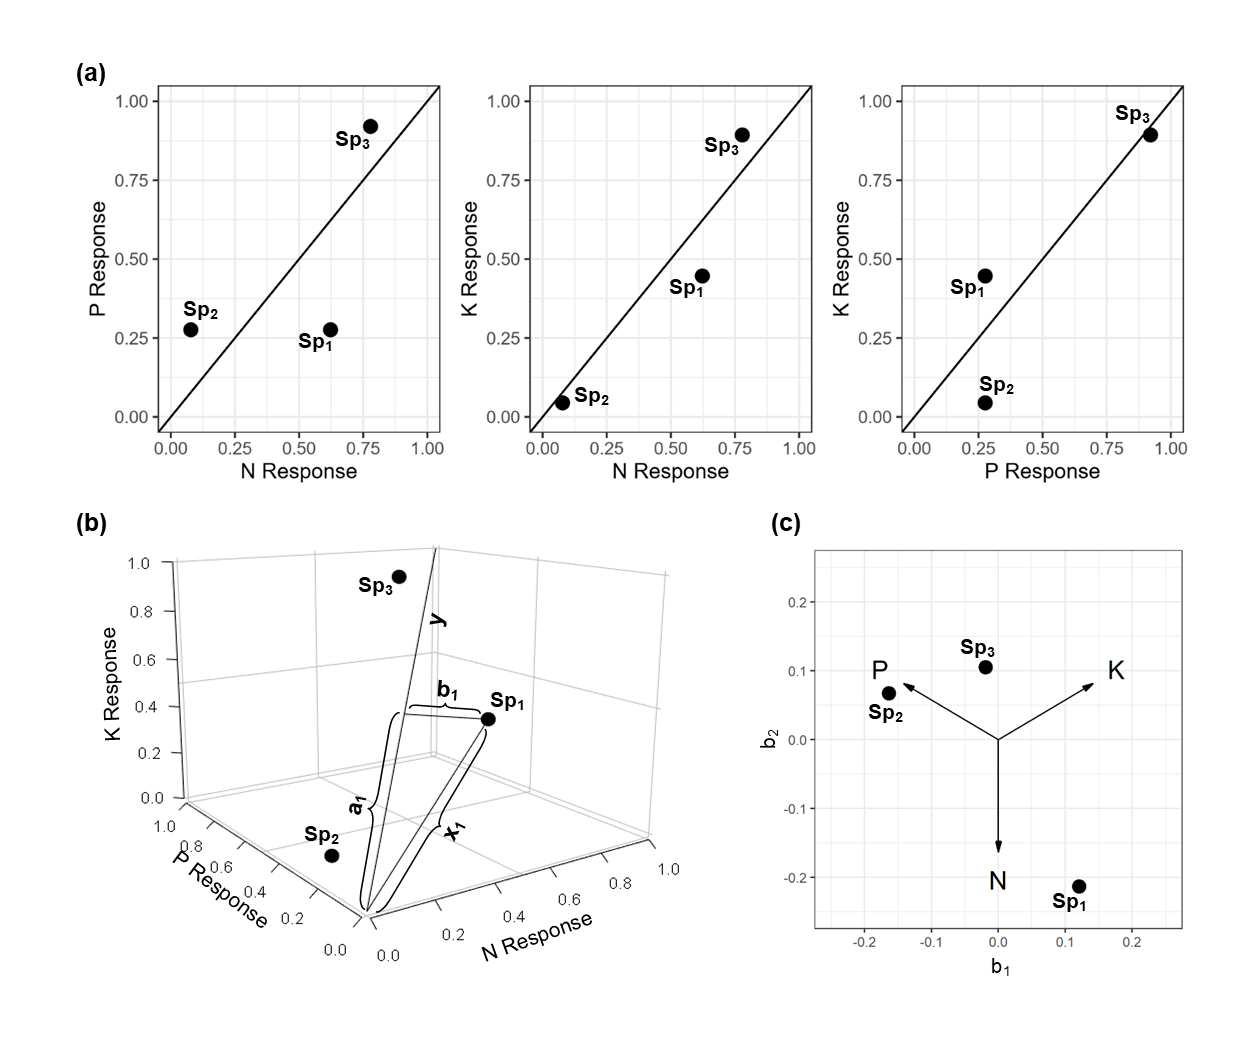
\includegraphics[width=\textwidth,height=0.6\textheight]{figure/Fig1_1.png}
\caption{Conceptual diagram illustrating the method used to assess dimensionality of community enrichment response. \newline (a) Bivariate relationships between responses: In this hypothetical example, a community of 3 species is subject to enrichment by three different resources. Estimated responses to these nutrients are standardized such that the total magnitude of community response to each nutrient is of unit length. The line illustrates the null hypothesis of proportionally identical responses; Species 1 (Sp1) exhibits comparatively stronger responses to N treatment than either P or K. \newline (b) Three-dimensional representation of responses: The responses above are presented as a three-dimensional plot, with the vector y representing the null hypothesis. The vector of responses estimated for Sp1, x1, is projected onto y, producing the projection, \(a_1\), and rejection, \(b_1\). The coordinates of this projection vector, \(a_1\), correspond to the average response of Sp1 recorded across all three nutrients. Projection and rejection vectors for Sp2 and Sp3 may be calculated in a similar fashion and used to evaluate response dimensionality at the community scale. In this community, strong positive correlation across all three treatment dimensions yielded low overall response dimensionality, D = 0.04. \newline (c) Two-dimensional plot of rejection vectors: Residual elements of the response vector not captured by projection onto y may be visualized in two dimensions, b1 and b2. Corresponding to relationships shown in bivariate plots, rejection elements of Sp1 have large values in the second rejection dimension, b2, reflecting proportionally stronger responses to N enrichment than other treatments. \label{fig-1-1}}
\end{figure}
While multivariate linear modelling approaches may be used to estimate the rate of community change in response to treatment, their output does not provide a quantification of similarity among directions of change. To evaluate correlations among different trajectories of community response -- proportional consistency across the responses of individual species that contribute to overall community response -- we derive a geometric approach based on work of ({\textbf{???}}).

In the context of this study, we evaluate trajectories of community change based on experimental manipulations of three limiting nutrients -- N, P, and Kµ. While the following description presents details for this three-dimensional case, our approach may extend to any n-dimensional set of treatments. First, we define \(\mathbf{X}\) as a matrix describing the treatment responses (columns) of all \(S\) species observed in a community (rows). For simplicity in notation, we define each row vector consisting of the \(i\)th species responses to different treatments as \(x_i\); column vectors describing the response of all species within the \(j\)th community to a given treatment as \(x_{:,j}\).

\[
\mathbf{X} = 
\begin{matrix}
Sp & Trt_1 & Trt_2 & Trt_3\\
\hline
\mathbf{1}& x_{1,1} & x_{1,2} & x_{1,3} \\
\mathbf{2} & x_{2,1} & x_{2,2} & x_{2,3} \\
\vdots & \vdots & \vdots & \vdots \\
\mathbf{S} & x_{S,1} & x_{S,2} & x_{S,3} \\
\end{matrix} =
\begin{matrix}
\\
\mathbf{x}_1 \\
\mathbf{x}_2 \\
\vdots \\
\mathbf{x}_S \\
\end{matrix} \\
= \\
\begin{matrix}
\mathbf{x}_{:,1} & \mathbf{x}_{:,2} & \mathbf{x}_{:,3}\\
\end{matrix}
\]

In this study, \(\mathbf{X}\) was composed of the three vectors of estimated nutrient response coefficients computed in multiple regression model, B.We captured to total magnitude of compositional change in response to treatments using the Euclidean (\(L_2\)) norm of column (treatment response) vectors, defined as:

\[\|\mathbf{x}_{:,j}\| = \sqrt{\sum_{i = 1}^{S} x_{i,j}^2}\]

Where \(i\) iterates over the \(S\) species present within each community.

To control for differences in magnitudes of change across treatments, column vectors were standardized through dividing by \(L_2\) norm, such that \(\|x_{:,j}\| = 1\). After standardization, community responses to treatment are equal in length, allowing for comparison between directions of change.

To compare potential trade-offs among different axes of environmental change, bivariate relationships may be used to illustrate correlated patterns of change between pairs of treatments (Figure 1a). To evaluate these bivariate relationships, we fit Semi Major Axis (SMA) regressions to each pairwise combination of treatments, which account for uncertainty in both \(X\) and \(Y\) variables not captured in Ordinary Least Squares (OLS) regression.

However, bivariate relationships do not provide an aggregate measure of similarity among variables in 3 or more dimensions. Instead, correlation among responses can be evaluated through projection onto a new coordinate basis. Conceptually, our approach is similar to dimensionality reduction through Principal Component Analysis (PCA). Rather than defining the first Principle Component through eigenvalue decomposition, axes are pre-specified under a null hypothesis. We define this null model as a ``neutral'' expectation where the effects of nutrient enrichment are one-dimensional, resulting in trajectories of community change that are directionally equivalent. While the total magnitude of effect may vary, our null model assumes that species exhibit proportionally equal responses to multiple nutrient enrichment treatments.

First, we define a vector of 1's, \(\mathbf{y}\), to form an estimate of species responses under our ``neutral'' null hypothesis. Under this neutral expectation, proportionally equal responses to treatment will be perfectly captured by variation along this 1:1:1 vector (Figure 1b).

To evaluate the degree to which this null hypothesis captures the responses of species i, we define a vector, a, as the projection of observed responses onto the 1:1:1 vector, \(\mathbf{y}\):

\[\mathbf{a}_i = \frac{\mathbf{y} \cdot \mathbf{x}_i}{\|\mathbf{y}\|}\]

The orthogonal compliment of the projection, \(\mathbf{b}\), defines the elements of \(\mathbf{x}\) not captured by projection onto \(\mathbf{y}\):

\[\mathbf{b}_i = \mathbf{x}_i - \mathbf{a}_i\]

The fraction of variance in species response that is captured by this projection is thus defined as the ratio of squared norms (sums of squares) of \(\mathbf{a}\) and \(\mathbf{x}\):

\[D = 1 - \frac{\|\mathbf{a}_i\|^2}{\|\mathbf{x}_i\|^2}\]

Under our null hypothesis, the set of responses observed for species \(i\), \(\mathbf{x}_i\), will be of equal magnitude to the projection, \(\mathbf{a}_i\),. The proportional magnitude of these vectors thus serves as a measure of response dimensionality for a given species, \(i\).

Extending this method to all \(S\) observed species gives an aggregate measure of community dimensionality, bounded between 0 and 1:

\[D = 1 - \frac{\sum_{i = 1}^{S}\|\mathbf{a}_i\|^2}{\sum_{i = 1}^{S}\|\mathbf{x}_i\|^2}\]

Where dimensionality (\(D\)) is equal to one minus the ratio of summed magnitudes of change when projected on y over their observed magnitudes. When trajectories of community change are directionally identical (low dimensional), response vectors will be perfectly captured by this projection (\(D = 0\)). Orthogonal responses (high dimensional), where community responses to treatment are uncorrelated, will be poorly captured by this projection (\(D = 1\)).
When possible, elements of the rejection, \(\mathbf{b}\), may be used to visualize deviations from this 1:1:1 line (Figure 1c). In this study, we project this rejection component to two other dimensions orthogonal to \(\mathbf{y}\), constituting a change of basis. Thus, the overall projection onto y and residual coordinates may be expressed as \(XP^\top\), with projection matrix:

\[
\mathbf{P} = 
\begin{matrix}
y & b_1 & b_2 \\
\hline
0.577 & 0 & -0.816 \\
0.577 & -0.707 & 0.4082 \\
0.577 & 0.707 & 0.4082 
\end{matrix}
\]

Where column vectors above are standardized to unit length.

\emph{Structural Equation Modeling}

To capture variation in site-level community properties and abiotic characteristics, we generated a series of derived variables to supplement observations made during sampling. Climate characteristics were obtained from each site using BioClim, a publicly available dataset of global climate layers. Following prior analyses of the Nutrient Network dataset (Grace et al. \protect\hyperlink{ref-Grace2016a}{2016}), we chose to represent climatic effects on plant growth through site mean temperature at the wettest quarter of year (BIO8) and site mean precipitation during the warmest quarter of the year (BIO18).
Community properties were generated from compositional data collected during pre-treatment sampling. To estimate community spatial heterogeneity (``Species Turnover''), we calculated beta diversity using the ratio of site-level species richness to mean plot-level species richness (\(\beta=\frac{\gamma}{\alpha}\)). Pre-treatment community composition was also used to calculate the relative abundance of plant functional groups present within each site (e.g.~``Legume Abundance''), defined as the mean proportion of total cover across all plots. Estimates of the total site species pool (``Species Pool') were calculated by the total number of unique species observed in the first 5 years of sampling, to account for varying durations of observation across sites.
From sites with complete data (n = 35), we used structural equation modeling (SEM) to evaluate hypothesized links between environmental characteristics, community properties, and the dimensionality of community response to fertilization (``Response Dimensionality''). In our initial model, we specified pathways capturing site resource limitation and community characteristics. We incorporated pathways between composite variables describing soil nutrient availability (``Soil Resources'') and climatic conditions (``Climate'') on response dimensionality, also mediated through intermediate connections between community biomass (``Community Biomass'') and light availability (``Light Availability''). These same variables were also combined in pathways to estimate effects mediated by species turnover and the abundance of species in the legume functional group. After fitting this initial model, we evaluated model fit and pruned non-significant pathways to reduce model complexity.

\emph{Statistical Software}

All statistical analyses were performed in R version 4.0.2. Multivariate linear model fitting was conducted using RRPP (Collyer and Adams 2018). Semi-Major Axis (SMA) regression was performed using ``smatr'' (Warton et al.~2012). Linear mixed effects modeling was conducted using ``lme4'' and ``lmerTest'' packages (Bates et al.~2015, Kuznetsova et al.~2017). SEM analyses were conducted using ``lavaan'' (Rosseel 2012).

\hypertarget{results}{%
\section{Results}\label{results}}

\emph{Community Responses to Nutrient Enrichment}

Of the 49 sites included in analysis, 37 showed significant (P \textless{} 0.05) community responses to nutrient addition treatments (Figure 2a). While a majority of sites (30) exhibited significant effects of N enrichment, significant impacts of P (20) and Kµ (17 sites) addition were also common. Community rate of change per year of treatment was greatest in response to N enrichment. Once accounting for site-level variation in average effect, estimated mean magnitude of community change (in net Euclidean distance per year) was significantly greater following N fertilization than either P or Kµ (F2,96 = 4.8, P \textless{} 0.05; Appendix 2).
\begin{figure}
\centering
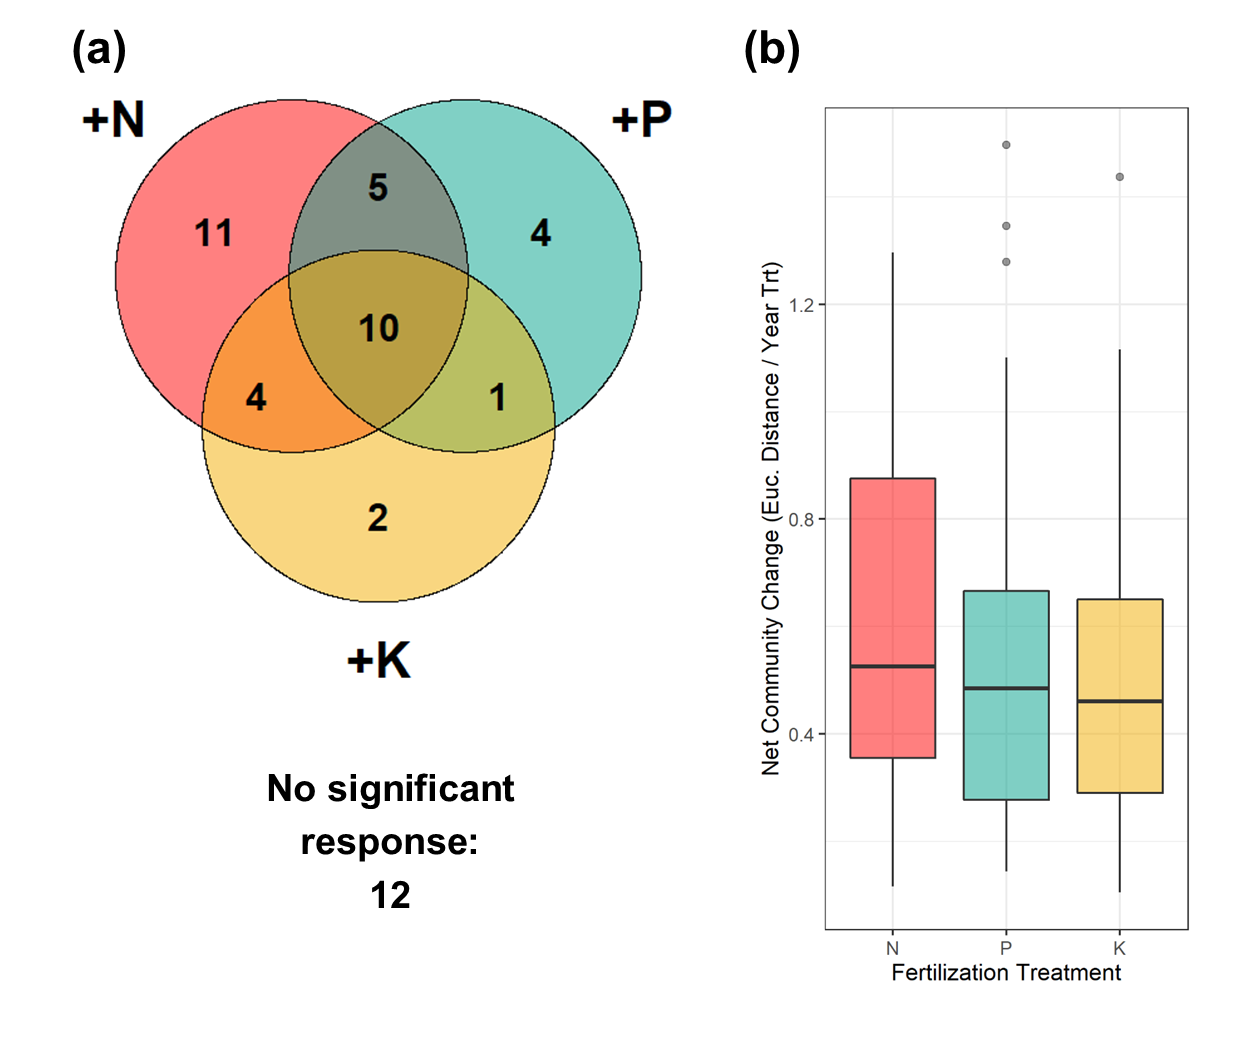
\includegraphics[width=\textwidth,height=0.6\textheight]{figure/Fig1_2.png}
\caption{\newline (a) Frequency of sites exhibiting significant (P \textless{} 0.05) effects of nutrient (N, P, or Kµ) fertilization on plant community composition. Of 49 total sites, 37 showed significant compositional changes to at least one of three fertilization treatments, while 12 sites showed non-significant compositional responses to all nutrient manipulations. \newline (b) Rate of estimated fertilization-driven change in species composition, prior to standardization of response coefficients. The rate of total compositional change was calculated as the magnitude of the vector of estimated species response coefficients, as net Euclidean change in log2-transformed community cover per year of treatment. Higher values indicate greater overall rate of compositional change. \label{fig-1-2}}
\end{figure}
\emph{Correlation Among Community Trajectories}

After standardizing overall community trajectories to unit length within each site, semi major axis (SMA) regression was used to evaluate correlations among responses to treatments at the species level. Pairwise comparisons between nutrient addition treatments (N-P, N-Kµ, P-Kµ) revealed positively correlated responses among all treatments, generally (Figure 3, Table 1). However, these relationships varied as a function of plant functional group. Small intercept terms and slope coefficients nearly equal to 1 indicate that Forb, Graminoid and Woody species exhibited relatively equal responses across all treatment comparisons. For these functional groups, SMA models captured a statistically significant portion of total response variance. High R2 values of Woody species, in particular, suggest that this group exhibit a more consistent trend than others, though this result should be interpreted with caution given their limited occurrence in our dataset (n = 18, Table 1).
In contrast, SMA regression fits to Legume species yielded slope coefficients and intercept terms that suggest stronger responses to P and Kµ treatments than would otherwise be predicted by response to N: positive intercept terms and slope coefficients greater than 1 produced when comparing responses to N and P treatments, for example, demonstrate the legumes exhibit more positive responses to P enrichment than N, which skew more strongly to P as total response magnitude increases (Figure 3, Table 1).
Repeated SMA regression with respect to plant dominance or longevity showed no consistent deviations from general positive correlation in response coefficients (Appendix 3).
\begin{figure}
\centering
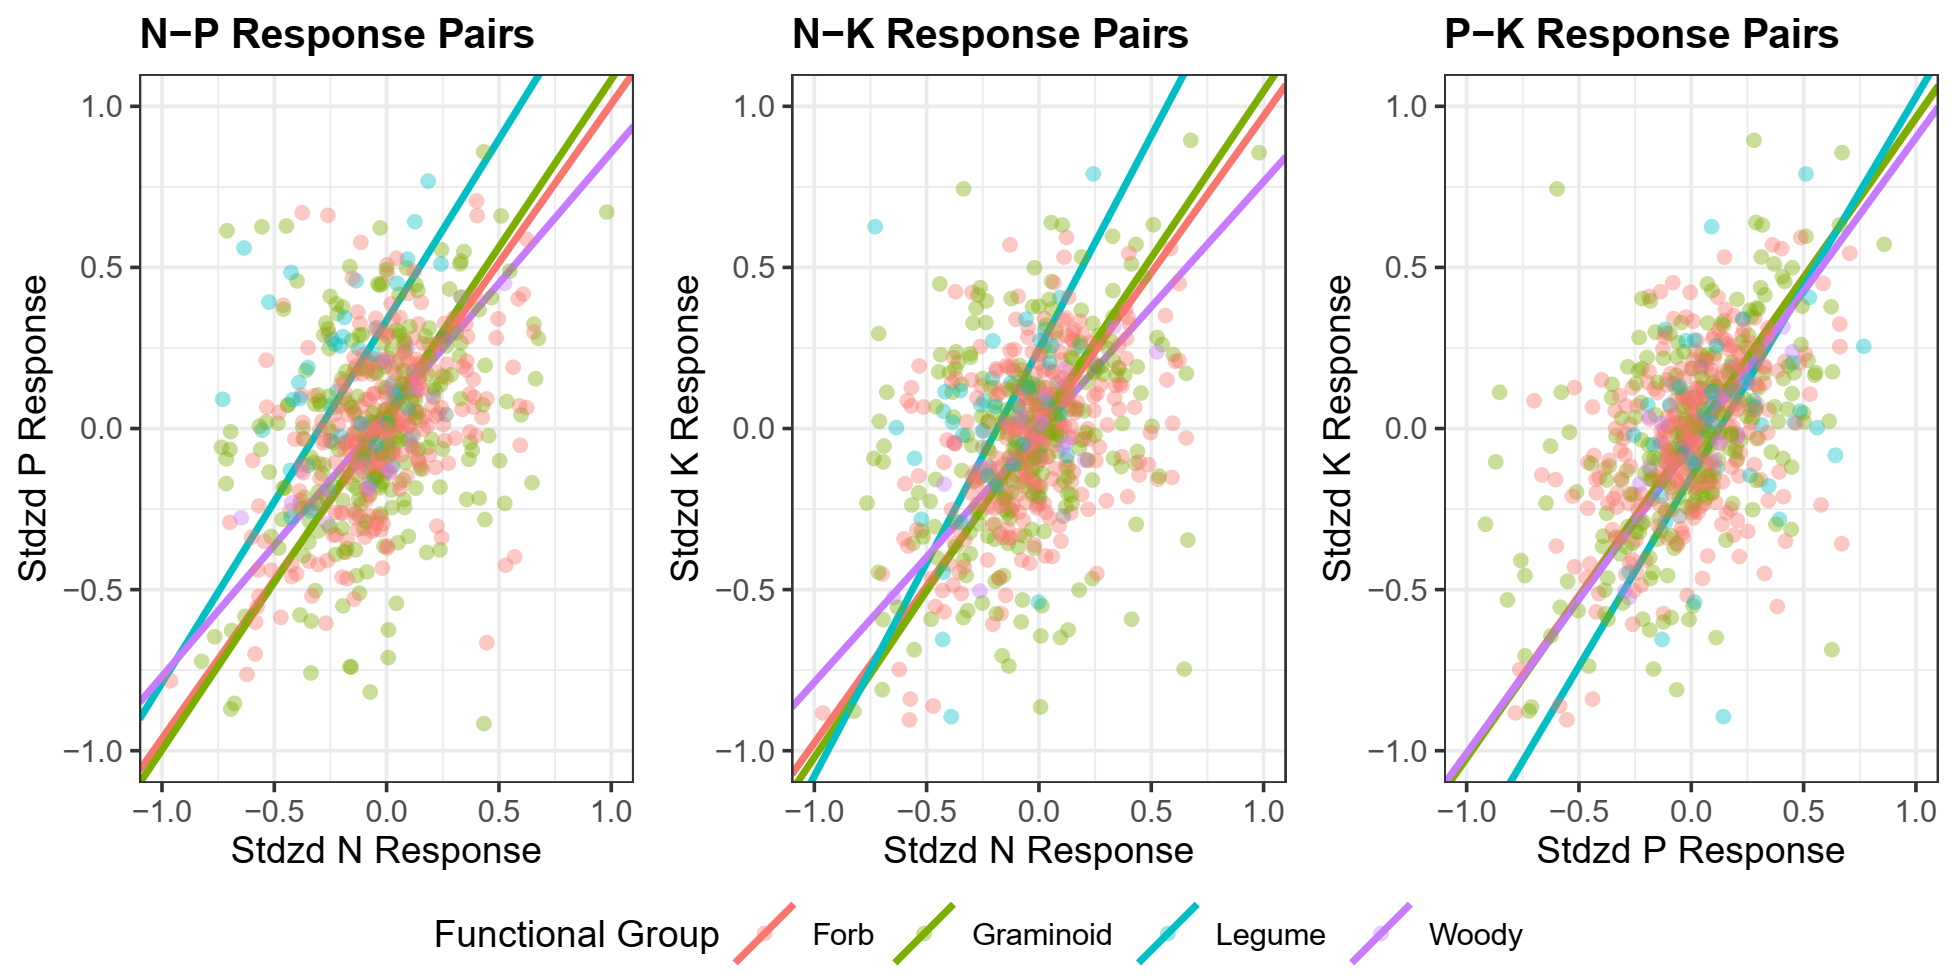
\includegraphics[width=\textwidth,height=0.35\textheight]{figure/Fig1_3.png}
\caption{Visualization of pairwise relationships between plant responses to nutrient addition treatments. Each point refers to a unique site x species combination, colored by functional group. Lines correspond to results of semi major axis (SMA) regression applied to each functional group. \label{fig-1-3}}
\end{figure}
\begin{table}[ht]
\centering
\begin{tabular}{llllll}
 Functional Group & Pair & n & Slope & Intercept & $R^2$ \\ 
  \hline
Forb & N-P & 307 & 0.99 & 0.02 & 0.20 \\ 
  Graminoid & N-P & 241 & 1.04 & 0.04 & 0.11 \\ 
  Legume & N-P & 46 & 1.13 & 0.34 & $0.032^{ns}$ \\ 
  Woody & N-P & 18 & 0.81 & 0.04 & 0.76 \\ 
   \hline
Forb & N-K & 307 & 0.97 & 0.00 & 0.21 \\ 
  Graminoid & N-K & 241 & 1.03 & 0.01 & 0.11 \\ 
  Legume & N-K & 46 & 1.33 & 0.25 & 0.10 \\ 
  Woody & N-K & 18 & 0.78 & -0.01 & 0.63 \\ 
   \hline
Forb & P-K & 307 & 0.99 & -0.03 & 0.21 \\ 
  Graminoid & P-K & 241 & 0.99 & -0.03 & 0.27 \\ 
  Legume & P-K & 46 & 1.18 & -0.15 & 0.09 \\ 
  Woody & P-K & 18 & 0.96 & -0.05 & 0.67 \\ 
  \end{tabular}
\caption{Summary of semi major axis (SMA) regression model fits to each of 3 pairwise comparisons of response to fertilization treatment. A majority of models captured significantly more variation (P < 0.05) in response than models assuming no correlation between treatment responses; models with non-significant fits are denoted by superscript “ns”.} 
\end{table}
\emph{Global Scale Response Dimensionality}

Across all sites and species, we found strong evidence that plant responses to fertilization treatments are characterized by a largely one-dimensional relationship. (Figure 4a). Projection of responses onto the y vector (assuming proportionally equal responses to treatment) captured 60.68\% of the total observed variance across all species; overall species response dimensionality, D, was equal to 0.29. This proportion is nearly identical to the fraction of variance captured by the first component in Principal Component Analysis (PCA) of our data, 60.77\%. Given that PCA attempts to transform data into a new coordinate basis that maximizes the fraction of variance present in the first component, projection onto the y vector under our null hypothesis achieves an equivalent fit to the best one-dimensional description of species responses to fertilization.
In line with observations made in pairwise comparisons, plant functional groups exhibited consistent patterns of deviation from the null hypothesis of proportionally consistent responses to treatment (Figure 4b, Table 2). While mean coordinates of plant functional groups did not differ significantly on either y or b1 dimensions, the mean coordinate position of Legume species on the second rejection dimension, b2, was significantly larger than the means of all other functional groups. Given the loadings specified in our projection, P, larger average coordinate values in this second rejection dimension are correlated with proportionally more positive responses to P or Kµ treatments than N enrichment.
\begin{figure}
\centering
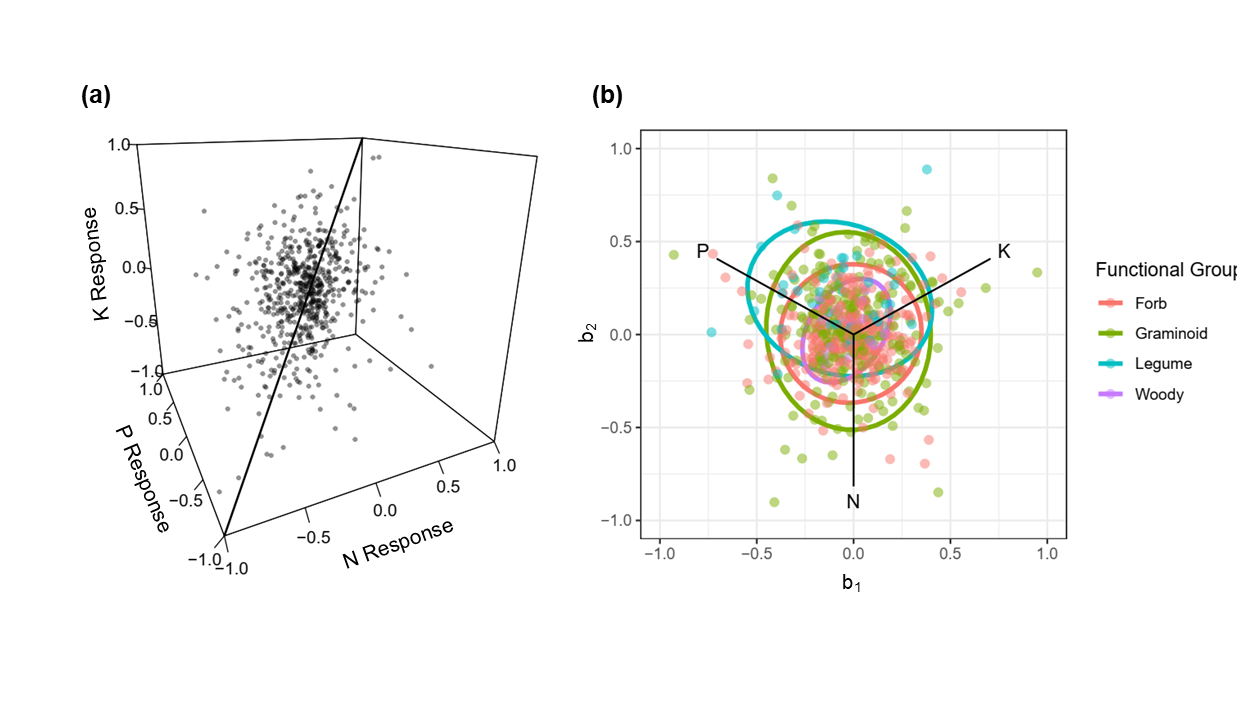
\includegraphics[width=\textwidth,height=0.45\textheight]{figure/Fig1_4.png}
\caption{\newline (a) Three-dimensional visualization of species responses to nutrient enrichment across all sites, with line corresponding to 1:1:1 vector (y) assuming proportionally equal responses. \newline (b) Residual deviation from 1:1:1 vector displayed in two dimensions (b¬1, b2) orthogonal to y. Points are colored by functional group with 95\% confidence ellipses centered on group means. \label{fig-1-4}}
\end{figure}
\begin{table}[ht]
\centering
\begin{tabular}{llll}
  \hline
 & $\bar{y}$ & $\bar{b_1}$ & $\bar{b_2}$ \\ 
  \hline
Forb & $-0.0331^1$ & $-0.0181^1$ & $0.0081^1$ \\ 
  Graminoid & $-0.0561^1$ & $-0.0211^1$ & $0.0021^1$ \\ 
  Legume & $-0.0051^1$ & $-0.0871^1$ & $0.2062^2$ \\ 
  Woody & $-0.0581^1$ & $-0.0371^1$ & $0.0221^1$ \\ 
   \hline
\end{tabular}
\caption{Mean coordinate position of functional groups along 1:1:1 vector ($\bar{y}$) and residual components ($\bar{b_1}$,$\bar{b_2}$). Superscripts correspond to significant (P < 0.05) contrasts between functional group means in each dimension.} 
\end{table}
\emph{Site Variation in Response Dimensionality}

To evaluate the environmental and community determinants of response dimensionality, we subdivided data by sites to calculate community response dimensionality, D, that captures variation in fertilization response across all observed species. Estimates D ranged between 0.08 and 0.73 (Mean = 0.39; Appendix 4).
Consistent with our hypotheses, SEM analysis identified significant relationships between soil resource availability, climatic characteristics, and response dimensionality (Figure 5). While increasing precipitation and lower growing season temperatures produced a positive, direct effect on response dimensionality, the effects of resource availability were primarily mediated through changes in average biomass and canopy light interception -- experiments performed in more productive environments characterized by stronger competition for available light were significantly correlated with greater variation in trajectories of community change across our three fertilization treatments.
Site species richness, soil resources, and climate also had effects on response dimensionality through changes in pre-treatment spatial turnover in species diversity (Figure 5). Less species turnover, estimated as spatial beta diversity of communities prior to treatment, and pre-treatment abundance of legumes combined to have negative effects on the dimensionality of community response to treatment. Community responses to fertilization treatment appear directionally varied in systems where N-fixing functional strategies are common and species diversity is likely to rely less on spatial coexistence mechanisms.
\begin{figure}
\centering
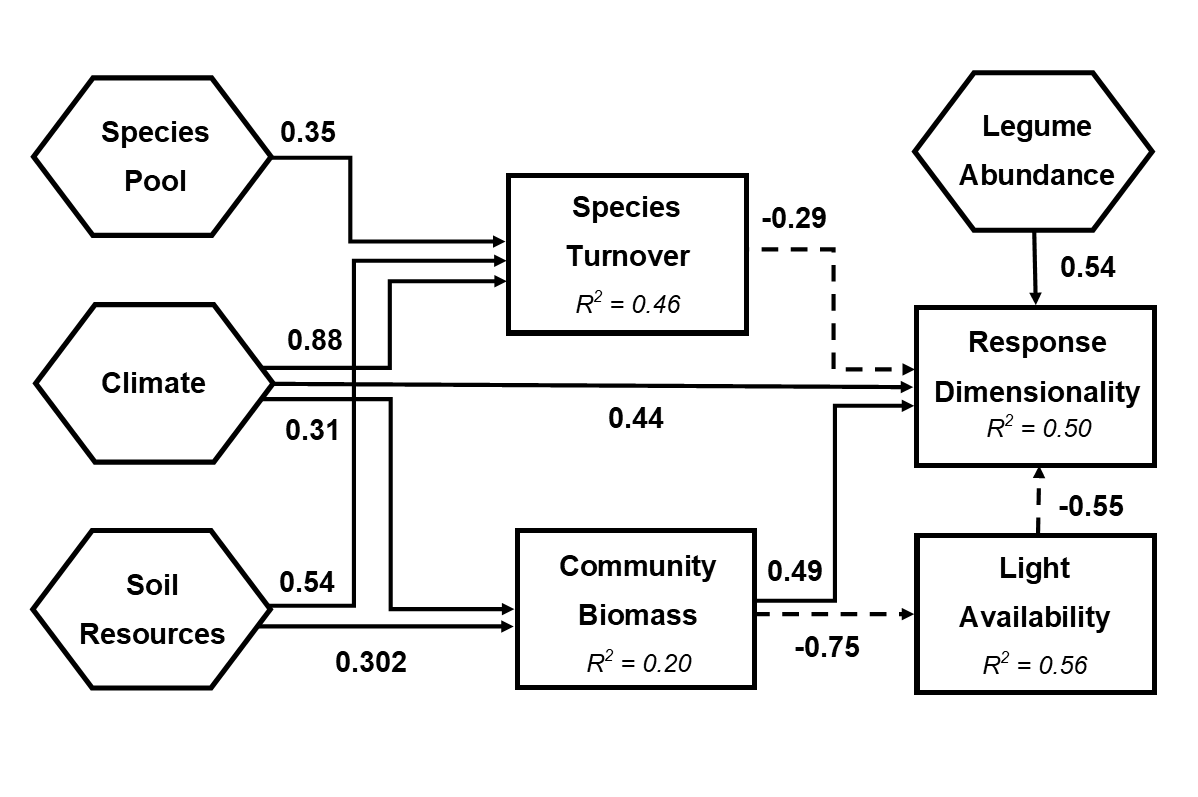
\includegraphics[width=\textwidth,height=0.5\textheight]{figure/Fig1_5.png}
\caption{Visual representation of structural equation model (SEM) used to evaluate pre-treatment site factors that explain variation in community response dimensionality (D) following multiple nutrient enrichment. All statistically significant (P \textless{} 0.05) pathways are presented. Solid lines correspond to positive effects, while dashed lines correspond to negative effects. Chi-square test statistic = 23.408 on 20 degrees of freedom indicates close model-data fit (P = 0.269; Comparative Fit Index = 0.943). \label{fig-1-5}}
\end{figure}
\hypertarget{discussion}{%
\section{Discussion}\label{discussion}}

In terrestrial plant communities, trade-offs among multiple niche axes are theorized to govern the coexistence of diverse, interacting species. Using data from a globally replicated experiment in grassland systems, we find support for the simultaneous contribution of two mechanisms -- a shift from belowground to aboveground resource limitation and multi-dimensional belowground tradeoffs -- that vary in their relative importance across sites.
Consistent with other studies of nutrient limitation in grassland systems, including those using data from the Nutrient Network experiment, we found that nitrogen enrichment produced greater average effects on composition than either phosphorous or potassium and micronutrient fertilization (Crawley et al. \protect\hyperlink{ref-Crawley2005}{2005}, Fay et al. \protect\hyperlink{ref-Fay2015}{2015}, Harpole et al. \protect\hyperlink{ref-Harpole2016}{2016}, Soons et al. \protect\hyperlink{ref-Soons2017}{2017}).

Given constraints on nitrogen fixation in many terrestrial systems (Vitousek and Howarth \protect\hyperlink{ref-Vitousek1991}{1991}), these results suggest that nitrogen availability may often act as a dominant niche axis of belowground resource availability. However, these findings may also be skewed by the disproportionate representation of Nutrient Network sites in temperate North America and Europe (Appendix 1). In arid environments and those composed of more weathered soils, plant demands for phosphorous and other micronutrients may exceed those of nitrogen (Handreck \protect\hyperlink{ref-Handreck1997}{1997}, Vitousek et al. \protect\hyperlink{ref-Vitousek2010}{2010}); experimental sites in Australia, for example, often exhibited the strongest community responses to phosphorous enrichment, on average (Appendix 4).
Surprisingly, 24 percent (12 of 49) sites did not respond significantly to any of the three resource enrichment treatments, despite addition at a rate much greater than natural fluxes (({\textbf{???}}); Vitousek et al. (\protect\hyperlink{ref-Vitousek2010}{2010}); Appendix 4). This finding may be linked to other sources of resource limitation; qualitatively, sites with low precipitation (and likely higher interannual community turnover) appear more likely to exhibit non-significant responses to treatment. However, this may also be the result of our conservative analytical approach that first accounts for spatial and temporal variation in site community composition before testing for fertilization effects.
After controlling for differences in the total magnitude of compositional change, directional comparison found support for a strongly one-dimensional pattern of variation at a global scale. The dominance of a single axis of variation implies the presence of a general trade-off between plant performance in low or high nutrient conditions, likely driven by asymmetric competition for light (Dybzinski and Tilman \protect\hyperlink{ref-Dybzinski2007a}{2007}, DeMalach et al. \protect\hyperlink{ref-DeMalach2017a}{2017}). This result supports other findings that identify light limitation as a primary mechanism of fertilization-driven compositional change ({\textbf{???}}, Hautier et al. \protect\hyperlink{ref-Hautier2018}{2018}).
More broadly, our results likely reflect differentiation across a ``fast-slow'' economic spectrum of adaptation (Reich \protect\hyperlink{ref-Reich2014}{2014}). Absent other drivers, such as disturbance, herbivores, or pathogens, we find evidence that plant growth strategies increase performance under high soil nutrient conditions, generally, as opposed to nutrient-specific trade-offs ({\textbf{???}}, Grime \protect\hyperlink{ref-Grime1974}{1974}). Physiological requirements of primary producers are known to be largely consistent in stoichiometry (Ågren \protect\hyperlink{ref-Agren2004}{2004}, \protect\hyperlink{ref-Agren2008}{2008}), and as a result, interacting species are more likely to vary in total resource demand, rather than affinity for specific soil nutrients. The development of resource-specific trade-offs appears an unlikely coexistence strategy in many grassland systems. In response to other environmental changes, functional strategies that promote growth across multiple niche dimensions appear common -- grassland plant responses to elevated fertility and herbivore exclosure are generally correlated (Lind et al. \protect\hyperlink{ref-Lind2013}{2013}), and exhibit similar shifts in abundance across treatments removing different herbivore groups (Seabloom et al. \protect\hyperlink{ref-Seabloom2018}{2018}).
Despite the strength of a one-dimensional relationship across all species, we also found key deviations from this pattern based on plant functional strategies and site-specific contexts. In all sites, species in the Legume functional group responded more positively to potassium and phosphorous addition than nitrogen enrichment. While we still observed generally correlated patterns of change among these species, our findings suggest that nitrogen fixation may provide an additional advantage to effective competitors when other resources are supplied (Bobbink (\protect\hyperlink{ref-Bobbink1991}{1991});Suding et al. (\protect\hyperlink{ref-Suding2005}{2005}), Tognetti et al.~\emph{in review}) . Enzymatic costs of nitrogen fixation, which result in steeper requirements for phosphorous, potassium, sulfate, and other micronutrients relative to other plant functional types, may also contribute to this response (McKey \protect\hyperlink{ref-McKey1994}{1994}).
In turn, pre-treatment legume abundance served as an important predictor of site-level response dimensionality. It appears likely that greater diversity in plant functional strategy at the species level contributes to more directionally varied responses within a community to fertilization by different nutrients (Díaz and Cabido \protect\hyperlink{ref-Diaz2001}{2001}). However, distinctions between legumes and non-legume species are relatively coarse, and likely do not capture other key sources of plant functional variation and their relationship with fertilization. Further exploration of the links between plant nutrient response and other key trait dimensions, such as the leaf economic spectrum (Wright et al. \protect\hyperlink{ref-Wright2004}{2004}), tissue stoichiometry (Güsewell \protect\hyperlink{ref-Gusewell2004}{2004}), and root physiology (Kramer-Walter et al. \protect\hyperlink{ref-Kramer-Walter2016}{2016}) may better distinguish species groups at a global level, as well as their relationship to site-specific effects.
At the site scale, we also found that community responses to fertilization treatments were strongly contingent on site-specific characteristics. Community variation in treatment response -- response dimensionality -- was positively correlated with a series of covariates related to pre-treatment patterns of resource limitation and community interactions. We found increased response dimensionality in sites with low light interception, high productivity, and low spatial community turnover. This suggests that trade-offs in the belowground nutrient use are more common in systems where coexistence is maintained through local competition. While not presenting a direct mechanistic link to plant resource use strategies, these findings are supported by reports that functional trade-offs are often more constrained in stressful environments (Dwyer and Laughlin \protect\hyperlink{ref-Dwyer2017}{2017}). In grasslands, disturbance and climatic stress frequently act as strong habitat filters, and their fluctuations are known to serve as important mechanisms of species coexistence (Chesson \protect\hyperlink{ref-Chesson2000}{2000}, Adler et al. \protect\hyperlink{ref-Adler2006}{2006}). Under conditions where growing season precipitation strongly controls plant growth and fitness, for example, viable functional strategies are primarily distributed along a single axis related to relative growth rate and stress tolerance (Angert et al. \protect\hyperlink{ref-Angert2009}{2009}).
Like all studies exploring plant responses at the community, our results are subject to the properties of unique community assemblages occurring at each site. While able to infer some of these properties based on aggregate community attributes, such as biomass and functional group abundance, our results do not provide a link to species-level responses. Moreover, by limiting our analysis to species with well-characterized abundance shifts following fertilization, we necessarily exclude transient ones. These species can have important roles governing community response to nutrient enrichment and may exhibit functional strategies that are distinct from more persistent taxa (Wilfhart et al.~\emph{in review}).
Together, our findings present evidence for a generally one-dimensional axis of variation in plant response to fertilization, yet underscore the importance of site-specific constraints. Outcomes of plant competition for limiting soil nutrients are best predicted by relative differences in resource use ({\textbf{???}}), and represent a subset of many potential axes of niche differentiation (Kraft et al. \protect\hyperlink{ref-Kraft2015}{2015}). As a result, the relative contribution of trade-offs mediated by light competition or competition for individual belowground resources will depend on the unique set of factors structuring community interactions in each context.
Just as functional diversity and environmental characteristics are known to control ecosystem sensitivity global change, this study suggests that these same factors likely influence what mechanisms govern plant community response. Consideration of the direction of community change across multiple stressors thus forms an important complement to differences in their magnitude. Given that many ecosystems are subject to many global changes simultaneously, nuanced understand of their effects depends on identifying the trade-offs on which they operate. Stressors applied in tandem often have additive or super-additive effects on plant diversity and community composition (Zavaleta et al. \protect\hyperlink{ref-Zavaleta2003}{2003}, Harpole et al. \protect\hyperlink{ref-Harpole2016}{2016}, Komatsu et al. \protect\hyperlink{ref-Komatsu2019}{2019}), though effect sizes alone do not indicate whether communities shift along one dimension or several. While plant responses to nutrient enrichment may be captured along a single axis in general, broad assumptions of community dynamics are unlikely to apply in all contexts. Instead, we emphasize that cross-site comparisons and deep consideration of the unique factors shaping compositional responses to global change are essential to effective management and conservation of ecosystem diversity and function.

\hypertarget{nitrogen-enrichment-has-scale-dependent-effects-on-plant-diversity-in-california-grasslands.}{%
\chapter{Nitrogen enrichment has scale-dependent effects on plant diversity in California grasslands.}\label{nitrogen-enrichment-has-scale-dependent-effects-on-plant-diversity-in-california-grasslands.}}

\chaptermark{Scale dependence}

Evan E. Batzer\textsuperscript{1*} and Valerie T. Eviner\textsuperscript{1}
\begin{enumerate}
\def\labelenumi{\arabic{enumi}.}
\tightlist
\item
  Department of Plant Sciences, University of California, Davis
\end{enumerate}
\begin{figure}
\centering
\includegraphics[width=0.3\textwidth,height=\textheight]{figure/Fig2_1.png}
\caption{\label{fig-2-1}}
\end{figure}
\begin{figure}
\centering
\includegraphics[width=\textwidth,height=0.4\textheight]{figure/Fig2_2.png}
\caption{\label{fig-2-2}}
\end{figure}
\begin{figure}
\centering
\includegraphics[width=\textwidth,height=0.4\textheight]{figure/Fig2_3.png}
\caption{\label{fig-2-3}}
\end{figure}
\begin{figure}
\centering
\includegraphics[width=\textwidth,height=0.4\textheight]{figure/Fig2_4.png}
\caption{\label{fig-2-4}}
\end{figure}
\begin{figure}
\centering
\includegraphics[width=\textwidth,height=0.4\textheight]{figure/Fig2_5.png}
\caption{\label{fig-2-5}}
\end{figure}
\begin{figure}
\centering
\includegraphics[width=\textwidth,height=0.4\textheight]{figure/Fig2_6.png}
\caption{\label{fig-2-6}}
\end{figure}
\hypertarget{climate-drives-transitions-between-vegetation-states-in-california-grasslands.}{%
\chapter{Climate drives transitions between vegetation states in California grasslands.}\label{climate-drives-transitions-between-vegetation-states-in-california-grasslands.}}

\chaptermark{Vegetation state transitions}

Evan E. Batzer\textsuperscript{1*},
Carolyn Malmstrom\textsuperscript{2},
and Valerie T. Eviner\textsuperscript{1}
\begin{enumerate}
\def\labelenumi{\arabic{enumi}.}
\tightlist
\item
  Department of Plant Sciences, University of California, Davis, USA
\item
  Department of Plant Biology, Michigan State University, East Lansing, MI, USA
\end{enumerate}
\hypertarget{abstract}{%
\section{Abstract}\label{abstract}}

Climate change is forecast to influence plant community composition through shifts in climate variability and increased frequency of extreme events.
In arid- and semi-arid grassland systems, community turnover is known to depend on both climate conditions and historical contingency, where prior community configurations affect future dynamics.
These contingencies are likely to act as an important driver of vegetation responses to climate events; their capture may enhance forecasts of community change and identify targets for active management.
In this study, we planted various California grassland plant community types and observed changes in their composition during a ten-year period that included a drought of historic magnitude, followed by one of the wettest years on record. Using algorithmic partitioning methods and multistate modeling, we evaluated both the number of discrete vegetation types that best captured community turnover and the probability of transition between them.
We found that compositional variance was best partitioned in 4 discrete groups, distinguishing between two sets of annual grasses often considered as one species group in expert models.
Moreover, vegetation states differed in their persistence under variable climate conditions, and often exhibited directional patterns of transition.
Certain vegetation states, such as communities dominated by native perennial grasses, demonstrated strong persistence across a range of climatic conditions;
persistence of others, including invasive annual grasses, exhibited linear relationships with precipitation.
These findings indicate that ecosystem resilience may be enhanced by certain vegetation states, while eradication efforts are likely to be most effective when climate conditions are favorable.
Quantification of the unique properties of community states may greatly improve models of community dynamics under a changing climate in grassland systems.

\hypertarget{introduction}{%
\section{Introduction}\label{introduction}}

Across ecosystems, climate change forecasts emphasize the increasing frequency of extreme events, in addition to changes in average climatic conditions (IPCC \protect\hyperlink{ref-IPCC2014}{2014}).
Changing climatic extremes are important drivers of compositional dynamics, responsible for shifts in species distributions, invasion events, and biodiversity loss (Smith \protect\hyperlink{ref-Smith2011b}{2011}, Felton and Smith \protect\hyperlink{ref-Felton2017}{2017})

As ecological communities are increasingly subject to climate patterns outside historical bounds of variation, capturing the effects of unprecedented climatic extremes will be critical to generating new paradigms for conservation and management (Hobbs et al. \protect\hyperlink{ref-Hobbs2009}{2009}).
However, given the complexity of many factors that control species abundances, these changes are often difficult to predict.

While species may exhibit varied tolerances to conditions imposed by heatwaves, droughts, and extreme cold, climate-driven changes in species relative abundances are also constrained by local interactions that govern community assembly (Tylianakis et al. \protect\hyperlink{ref-Tylianakis2008}{2008}, Fukami \protect\hyperlink{ref-Fukami2015}{2015}).
Compensatory responses to climate change, for example, may be limited by competitors that inhibit growth and colonization (Alexander et al. \protect\hyperlink{ref-Alexander2015}{2015}).
At the community scale, such local interactions depend on key emergent properties that vary as a function of community attributes, including species richness, functional diversity, or dominant taxa (Chapin et al. \protect\hyperlink{ref-Chapin1997}{1997}, Emery and Gross \protect\hyperlink{ref-Emery2007}{2007}).
As a result, short-term compositional responses to climatic events are likely to depend on prior community configuration, where the responses of different species assemblages vary in magnitude and direction (Fukami \protect\hyperlink{ref-Fukami2015}{2015}).

These complex interactions between climatic drivers and species assemblages are often summarized through conceptual models (Ogden et al. \protect\hyperlink{ref-Ogden2005}{2005}, Galatowitsch \protect\hyperlink{ref-Galatowitsch2012}{2012}).
Models of arid- and semi-arid systems emphasize the importance of historical contingency in community assembly, where vegetation is often characterized by non-equilibrium dynamics.
In these systems, applied ecologists often make management recommendations on ``state-transition models'' that identify the properties of different species groups (``states'') and their likely direction of change under various contexts (``transitions''; Bestelmeyer et al. \protect\hyperlink{ref-Bestelmeyer2003}{2003}).
In response to changing climate patterns, managers may use these models to predict which community states are likely to persist under climate extremes or reduce incursion of unfavorable vegetation types.

Long-term monitoring, particularly under changing conditions, provides an important way to evaluate and refine conceptual models.
As climate change effects continue to mount, management efforts are expected to increasingly rely on these models to predict vegetation dynamics under ``no-analog'' conditions (Williams and Jackson \protect\hyperlink{ref-Williams2007}{2007}, Hobbs et al. \protect\hyperlink{ref-Hobbs2009}{2009}).
However, the emergence of novel species assemblages and non-intuitive mechanisms of change may complicate the use of classic models, which are often based on qualitative observation by experts.
Instead, climate change will likely increase the demand for data-driven approaches (Allen-Diaz and Bartolome \protect\hyperlink{ref-Allen-Diaz1998}{1998}, Bartolome et al. \protect\hyperlink{ref-Bartolome2008}{2008}).
Though still limited by available observations, these computational methods may better capture potential mechanisms of change and rapidly update predictions as new information becomes available.
In grassland systems, clustering algorithms have shown promise in tests of expert models and in the tracking of community responses to variable grazing regimes and species invasions (e.g.; Jackson and Bartolome \protect\hyperlink{ref-Jackson2002a}{2002}\protect\hyperlink{ref-Jackson2002a}{a}, Stein et al. \protect\hyperlink{ref-Stein2016}{2016}, Stringham et al. \protect\hyperlink{ref-Stringham2003}{2003}). However, there appear to be few tests of their application to climate-driven vegetation turnover.

California grasslands have long been a focal system in the study of non-equilibrium dynamics.
In California, climate change is predicted to produce a 50\% increase in the frequency of extreme events by the end of the 21st century (Yoon et al. \protect\hyperlink{ref-Yoon2015}{2015}).
California grasslands are particularly sensitive to climatic extremes, given compositional dynamics defined by a predominantly annual life history, climate sensitivity (Hobbs et al. \protect\hyperlink{ref-Hobbs2007}{2007}), non-hierarchical competitive relationships (Uricchio et al. \protect\hyperlink{ref-Uricchio2019}{2019}), and strong priority effects (Young et al. \protect\hyperlink{ref-Young2014}{2014}).
In this system, state-transition models often decompose compositional turnover into variation between three species groups defined by shared life history strategy and history of colonization: (1) naturalized exotic annual grasses and forbs, (2) native perennial grasses and forbs, and (3) recently invasive exotic annual grasses.

Compositional shifts in California grasslands are thought to be governed by differences in fecundity, phenology, and plant-soil feedbacks that characterize these species groups (Corbin et al. \protect\hyperlink{ref-Corbin2007}{2007}).
While this functional variation may govern responses to interannual climate variation (Pitt and Heady \protect\hyperlink{ref-Pitt1978}{1978}), communities composed of different dominant species may also exhibit emergent properties that constrain subsequent compositional change.
Invasive annual grasses, for example, produce thick litter layers that suppress competitor growth (DiTomaso et al. \protect\hyperlink{ref-DiTomaso2008}{2008}).
These litter feedbacks may enhance invasive grass persistence when future climatic conditions favor other species groups, particularly those that may exhibit limited recruitment capacity, such as native perennial grasses (Seabloom et al. \protect\hyperlink{ref-Seabloom2003}{2003}\protect\hyperlink{ref-Seabloom2003}{a}).

While warming average temperatures in California are forecast to produce increases in the distribution and abundance of annual grasses across the state (Sandel and Dangremond \protect\hyperlink{ref-Sandel2012}{2012}), the effects of changing climate variance are less understood.
Recent extreme climatic events, however, may provide insight into future vegetation dynamics.
A drought from 2011-2015, which included the driest period in recorded history, was observed to produce significant changes in the composition and diversity of many grassland communities (Harrison et al. \protect\hyperlink{ref-Harrison2015}{2015}, Prugh et al. \protect\hyperlink{ref-Prugh2018}{2018}).
This event provides a unique opportunity to test conceptual models of California grassland community dynamics through monitoring of species abundance changes across different vegetation types.

In turn, the capture of these contingencies may actively inform ecosystem management.
Often focused on the establishment of native species and reduction in invasive species abundances, management of California's grasslands under novel climatic conditions is likely to benefit from the application of modern computational tools to characterize vegetation change.
Quantitative description of community transitions between dominant species groups may supplement largely qualitative models generated during climatic norms. Are certain desirable species groups more resistant to variable climatic conditions than others? Can extreme climatic events provide opportunities for targeted management action?

Here, we assess interactions between community assembly and climatic variation on vegetation composition in California annual grasslands across a 10-year period encompassing extreme drought.
Using data from experimental plantings of three key grassland species groups -- naturalized annual, native perennial, and invasive annual grasses --- we test key assumptions of grassland community dynamics under extreme drought stress.
Specifically, we aim to identify (1) the species groups that best partition compositional change, and (2) how drought interacts with other drivers of vegetation turnover --- assembly order and biotic resistance --- to affect community composition.

\hypertarget{methods}{%
\section{Methods}\label{methods}}

\emph{Study site and Experimental Methods}

Plantings were conducted in research fields at the University of California, Davis (38.545751, -121.784780).
Previously used in crop production, these fields were left fallow from 1985 to the start of experimental plantings in 2007.
75\% of the experiment was set on Reiff series soil (coarse-loamy, mixed, superactive, nonacid, thermic Mollic Xerofluvents), with the rest on Brentwood soil series (fine, smectitic, thermic Typic Haploxerepts) with a 0-2\% slope (USDA Web Soil Survey).
The site has a Mediterranean climate, experiencing a mean annual rainfall of 457mm and mean daily temperature of 15.5 deg C between 1983-2018.

In order to minimize the previously established seedbank, soil was disked, irrigated to stimulate germination, and sprayed with a broad-spectrum herbicide (glyphosate). Irrigation and herbicide treatments occurred twice in the early fall of 2007.

Seeds were planted to establish vegetation treatments representing commonly used species groups in California's grasslands --- native perennial grasses and forbs (``native''), naturalized annual grasses and forbs (``naturalized''), and invasive annual grasses (``invasive''; Table 1 ).

Each group was planted alone, in all possible 2-group combinations, and all together in a 3-group combination.
Plots were 1.5m x 1.5m (2.25 m2), with 1m buffer between plots, and 8 replicates per treatment (56 plots total) laid out in a randomized block design.
In each plot, a total of 139 grams of seed was added, reflecting an average of 8,000 plants/m2 - a typical mature plant density in this system (Heady \protect\hyperlink{ref-Heady1958}{1958}).
For each monotypic community (e.g.~native vs.~invasive vs.~naturalized), an equal proportion of seeds of each species were added. For community mixtures, an equal proportion of community type seed was added (e.g.~in invasive + naturalized, 50\% invasive, 50\% naturalized seed), with equal proportion of individual species within each community type.

From 2008 - 2018, total areal cover of all species was estimated to the nearest 10\%. Cover observations for each species were performed in early and late spring to capture maximum percent cover for each species when varying in phenology. The highest percent cover value in each year for each species was used in analysis.
\begin{table}[ht]
\centering
\begin{tabular}{lll}
  \hline
Native & Naturalized & Invasive \\ 
  \hline
Acmispon americanus & Avena fatua & Aegilops triuncialis \\ 
  Bromus carinatus & Bromus hordeacous & Elymus caput-medusae \\ 
  Elymus glaucus & Festuca perennis var. multiflorum &  \\ 
  Elymus triticoides & Trifolium subterraneum &  \\ 
  Festuca microstachys &  &  \\ 
  Lupinus bicolor &  &  \\ 
  Poa secunda &  &  \\ 
  Stipa pulchra &  &  \\ 
   \hline
\end{tabular}
\caption{Results of indicator species analysis follow-
ing K-medoids clustering. High values of the indica-
tor species statistic reflect strong associations between a
taxon and a given state assignment. P-values calculated
using 1,000 permutations.} 
\end{table}
\emph{State Classification}

Prior to vegetation group classification, plant community observations were filtered to include only those species present within initial seeding mixtures and Bromus diandrus, a locally abundant annual grass that self-recruited into the experiment and is an important component of the California grassland type.
Despite regular weeding, a number of agricultural weeds (largely Convolvulus arvensis) occasionally recruited into plots from the seedbank and nearby fields and roadways over the course of our experiment.
Due to the effects of weeding and generally low abundance, these species were removed from community analysis.
The resulting dataset captured 93\% of the total vegetation abundance observed over the course of the experiment.

Algorithmic partitioning was used to determine core species groups that correlated in abundance over the course of our study.
It is important to note that partitioning is limited to the suite of observations made between 2008 - 2018, capturing n = 560 plot:year combinations.
This period includes a historic drought (2011-2015) and significantly wet year (2017), resulting in statistical groupings that are contingent upon the climatic regime and starting conditions imposed in experimental design.

Partitioning was performed using an unsupervised clustering algorithm, K-medoids clustering.
The K-medoids algorithm clusters data into k unique groups by identifying k medoid samples that best partition the total distance-based inertia of all observations.
Distance between observations was calculated using Bray-Curtis dissimilarity.

Because the number of relevant clusters in our study was not pre-defined, we applied K-medoids clustering across values of k from 2-10, yielding a number of clustering solutions.
We then compared the output of each of these clustering solutions using numerous tests---Hartigan, CH, Beale, KL, Cindex, DB, Silhouette, and Duda indices (Malika et al. \protect\hyperlink{ref-Charrad2014}{2014}).
The value of k with the best performance across all tests was chosen as the number of clusters that best represented vegetation partitions within this dataset.

Following the partitioning of states, we then conducted indicator species analysis to establish which species are associated with each state.
Indicator species analysis was performed using 9999 random permutations of state assignments to quantify statistical significance.
Clustering and diagnostics were generated using ``cluster'' (Maechler and others \protect\hyperlink{ref-Maechler2019}{2019}) and ``nbclust'' (Malika et al. \protect\hyperlink{ref-Charrad2014}{2014}).
Community analyses were performed using ``vegan'' (Oksanen et al. \protect\hyperlink{ref-Oksanen2016}{2016}).

\emph{Weather data}

To contextualize drought stress observed during our experiment, we quantified precipitation and evapotranspiration using data provided by a local California Irrigation Management Information System (CIMIS) monitoring station in Davis, CA (38.535694, -121.777636).
CIMIS automated dataloggers collect weather data on a minute-by-minute basis, including air temperature, soil temperature, precipitation, solar radiation, vapor pressure, and wind speed.
We aggregated these data into monthly intervals, where we calculated Standardized Precipitation-Evapotranspiration Index (SPEI).
This metric can be used to quantify the magnitude of drought stress relative to historic norms (Vicente-Serrano et al. \protect\hyperlink{ref-Vicente-Serrano2010}{2010}, Slette et al. \protect\hyperlink{ref-Slette2019}{2019}).

SPEI defines drought stress (\(D\)) at a given timepoint, \(i\):

\[
D_i = P_i - ETo_i
\]

Where represents observed precipitation and \(ETo_i\) represents estimated evapotransporation. ETo was calculated using the Penman-Monteith equation, defined as:

\[
ETo = \frac{\Delta(R_n - G) + \rho_a c_p \frac{e_s - e_a}{r_a}}{\Delta + \gamma(1 + \frac{r_s}{r_a})}
\]

Here, Rn is net radiation, \(G\) is soil heat flux, (\(e_s - e_a\)) is the vapor pressure deficit of air, \(\rho_a\) is the mean air density at constant pressure, \(cp\) is the specific heat of air, \(\Delta\) is the slope of the saturation vapor pressure temperature relationship, \(\gamma\) is the psychometric constant, and \(r_s\) and \(r_a\) are the surface and aerodynamic resistances (Vicente-Serrano et al. \protect\hyperlink{ref-Vicente-Serrano2010}{2010}).

To contextualize observed climate patterns relative to long-term variation, we calculated SPEI for a 35-year span between 2018 and 1983 (the first year that sufficient climate data was collected by the CIMIS system).
To account for potential temporal lag in the effects of climate variation on grassland species abundance (Sala et al. \protect\hyperlink{ref-Sala2012b}{2012}, Dudney et al. \protect\hyperlink{ref-Dudney2017}{2017}), we created drought indices across several cumulative water year durations.
For each year of available data, we calculated SPEI for a single water year (October -- May; 8 months), two consecutive water years (20 months), and three consecutive water years (32 months).
We then standardized these values by fitting the drought index series to a log-logistic distribution.
Resulting values of SPEI were centered at the mean drought stress across overall observations (\(D = 0\)), and individual years range between extreme droughts (\(D < -2\)) and significant water surplus (\(D > +2\)).

SPEI calculations were performed with the ``SPEI'' package (Beguería et al. \protect\hyperlink{ref-Begueria2014}{2014}).

\emph{Construction of Multistate Models}

To quantify the probability of vegetation transitions, we fit a multistate model (syn. Markov model) to community state assignments over time.
In this model, the probability that a given plot transitions from one vegetation state to another is estimated by a transition matrix, whose terms may also interact with different covariates.

We fit 8 candidate multi-state models to our data, beginning with a baseline model consisting of a transition matrix without influence of any covariates.
This base model was then further modified through inclusion of additional terms reflecting the influence of drought stress calculated over 1-, 2-, and 3-year intervals (SPEI), in addition initial planting composition (temporal priority effects).
Temporal priority was defined as a binary (1/0) variable describing whether indicator species of a given state were a component of the seeded species mixture.
We fit models consisting of only drought effects as covariates , temporal priority as a covariate, and models containing both drought and temporal priority as additive effects.

AIC scores were used to compare the relative fit of all potential candidate models. We selected the model with the lowest AIC score as our best fit model.
A table consisting of model descriptions and AIC scores is presented in Appendix 7. Multistate model fitting and model selection was performed using the ``msm'' package. (Jackson \protect\hyperlink{ref-Jackson2011}{2011})

All analyses were conducted in R version 3.06 (R Development Core Team).

\hypertarget{results}{%
\section{Results}\label{results}}

Seeding treatment effects on community composition

In the first year of observation (2008), plant communities were highly segregated as a function of seeded species mixture (PERMANOVA, pseudo-\(F_{6, 49} = 32.815, P < 0.001\); Appendix 1).
Pairwise contrasts of community dissimilarity indicate clear distinctions in vegetation group establishment following seeding -- all planting mixtures containing the ``naturalized annuals'' group were similar in their species composition, as were mixtures composed of ``invasive grasses'' and ``invasive grasses + native species''.
The single group ``native species'' treatment composition was also compositionally segregated from others.

Partitioning vegetation into discrete states

Community composition observed in 2008 - 2018 was highly dynamic.
On average, plant communities in the same plot compared in two consecutive years were observed to share roughly 50\% of their total relative species cover (mean Bray-Curtis dissimilarity = 0.52 +/- 0.01 standard error).
Clustering captured a substantial proportion of total compositional variation(Pseudo-\(R^2\) = 0.39; Figure 2).
However, residual variation suggests that fluctuations in cover within clusters were still common.
This indicates that our method best captured broad changes in the dominance of correlated groups of species, rather than the varying abundance of individual species.

Partitioning of community variance into vegetation states was best characterized by 4 discrete clusters (Appendix 2).
Indicator species analysis of these assignments demonstrated that 2 of 4 vegetation states largely followed established conceptions of vegetation types within this system (Figure 2).
State 1 (hereafter, Native Perennials) was characterized by a group of native perennial grasses, while State 3 (Invasive Annuals) was composed of the two planted invasive annual species.
However, State 2 (B. hordeaceus-Festuca Annuals) and State 4 (Avena-B. diandrus Annuals) reflected the partitioning of the ``Naturalized Annual'' group into two separate types.
Cluster assignments reflected a 75\% cumulative relative abundance of associated indicator species, on average. Less than one tenth of observations had cumulative indicator species relative abundances of less than 40\% (Appendix 3).
\begin{figure}
\centering
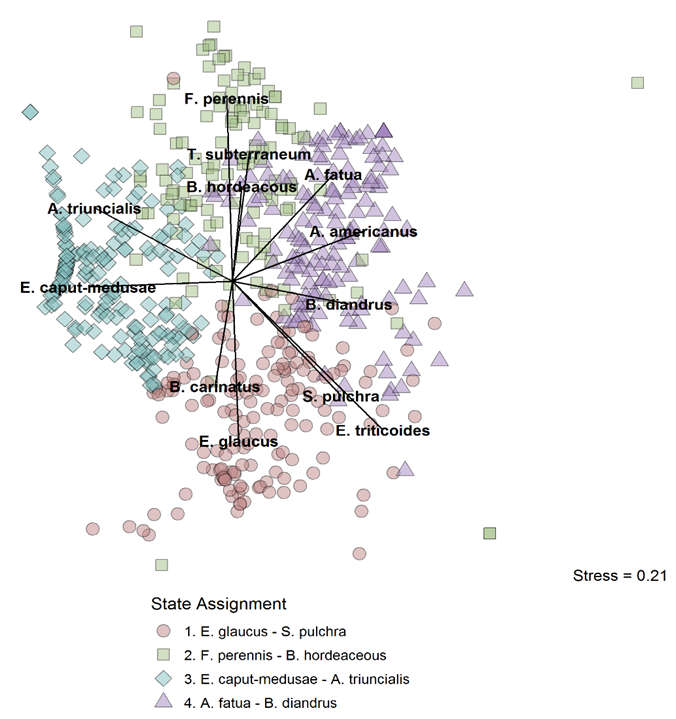
\includegraphics{figure/Fig3_2.png}
\caption{Visualization of clustering assignments following K-medoids clustering. Non-metric multidimensional scaling (NMDS) ordination was conducted on all community observations from 2008 -- 2018 (n=560). Pairwise community distance was calculated using Bray-Curtis dissimilarity index. Species vectors correspond to taxa that were found to be significantly associated (p \textless{} 0.05) with state assignments using indicator species analysis. \label{fig-3-2}}
\end{figure}
\begin{table}[ht]
\centering
\begin{tabular}{rlrr}
  \hline
State & Species & Statistic & P-value \\ 
  \hline
1.00 & E. glaucus & 0.80 & 0.00 \\ 
  1.00 & S. pulchra & 0.57 & 0.00 \\ 
  1.00 & B. carinatus & 0.55 & 0.00 \\ 
  1.00 & F. microstachys & 0.28 & 0.00 \\ 
  2.00 & F. perennis & 0.82 & 0.00 \\ 
  2.00 & B. hordeaceus & 0.72 & 0.00 \\ 
  2.00 & T. subterraneum & 0.61 & 0.00 \\ 
  3.00 & E. caput-medusae & 0.87 & 0.00 \\ 
  3.00 & A. triuncialis & 0.74 & 0.00 \\ 
  4.00 & A. fatua & 0.82 & 0.00 \\ 
  4.00 & B. diandrus & 0.55 & 0.00 \\ 
  4.00 & E. triticoides & 0.30 & 0.04 \\ 
  4.00 & A. americanus & 0.27 & 0.01 \\ 
   \hline
\end{tabular}
\caption{Results of indicator species analysis following K-medoids clustering. High values of the indicator species statistic reflect strong associations between a taxon and a given state assignment. P-values calculated using 1,000 permutations.} 
\end{table}
\emph{Frequency of state assignments over time}

The climatic conditions we observed included a period of normal to above-average water availability (2008 -- 2011), followed by drought (2012 -- 2016), and substantial water surplus (2017; Figure 1A).
During this period, community transitions between vegetation states were common in all plots (mean number of total transitions observed per plot = 3.73 +/- 0.16 SE).
The frequency of these transition events---summarized in a contingency table (Appendix 4)---were highly non-random, varying as a function of a plot's state assignment in a previous year, in addition to current climatic conditions (plot-level state assignments presented in Appendix 5).

Following seeding, a majority of communities were characterized by a single state assignment, as each of the 32 plots that received naturalized annual seed (including Avena fatua and Trifolium subterraneum) assumed the Festuca-B. hordeaceus state (Figure 1B).
The predominance of this community configuration was short-lived, however, and subsequent community dynamics were largely driven by a series of sequential, unidirectional transitions.
\begin{figure}
\centering
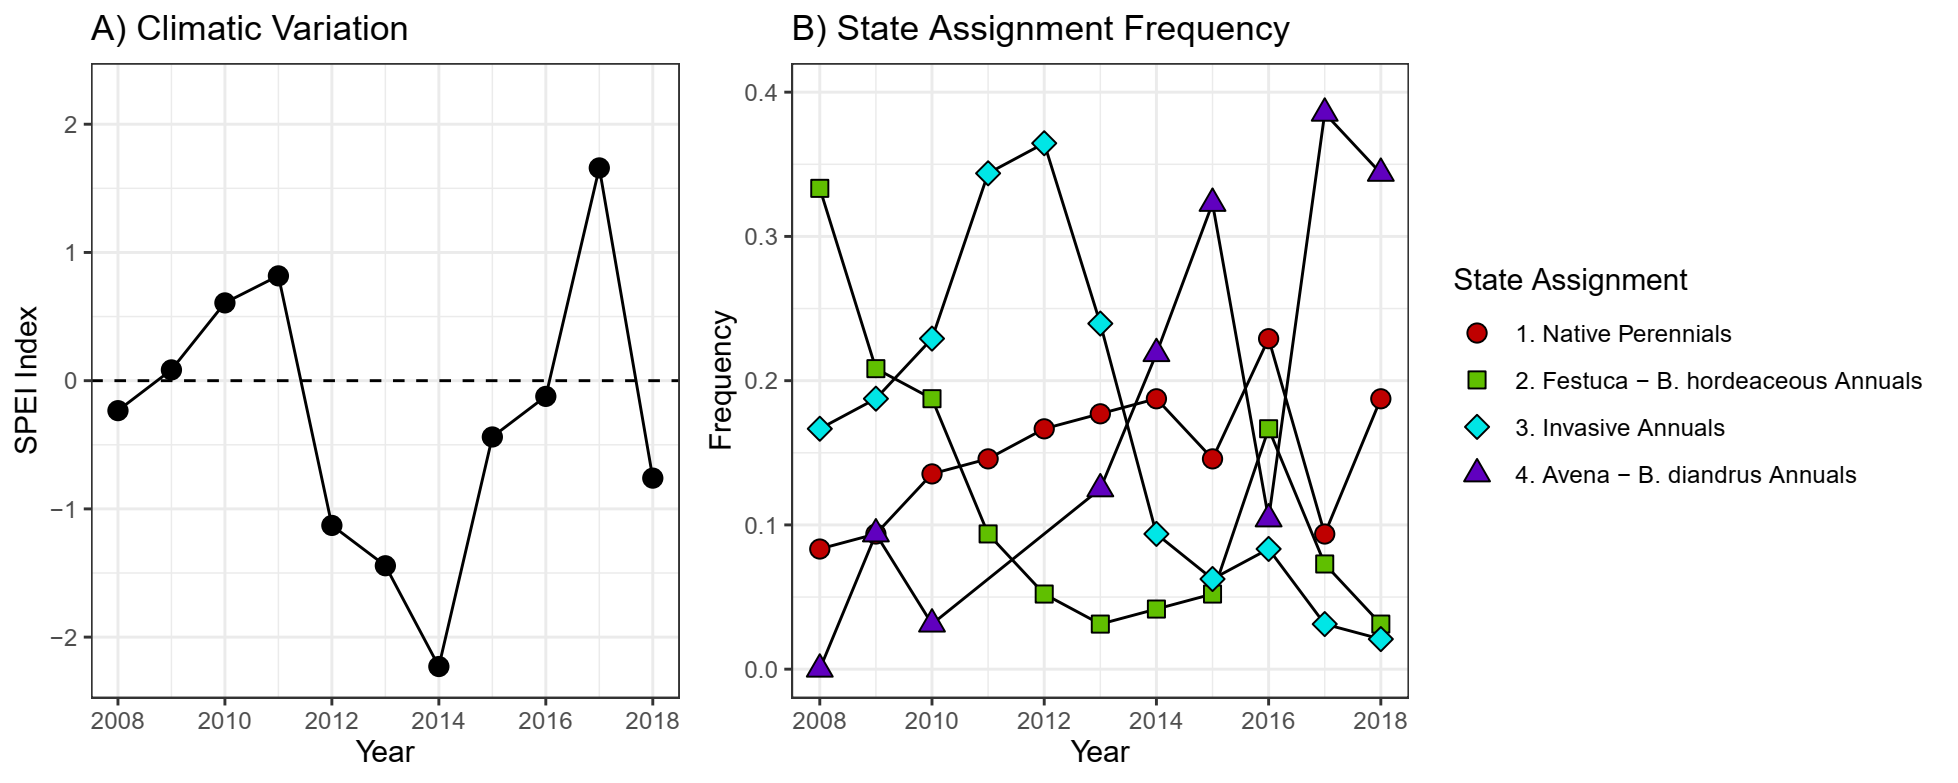
\includegraphics[width=\textwidth,height=0.3\textheight]{figure/Fig3_1.png}
\caption{Variation in total water year drought severity (A) and frequencies of state assignments (B) from 2008-2018. Average drought stress (SPEI = 0) between 1983-2008 is presented as a dotted line in panel A. Drought in California from 2012-2016 included several years of substantially below-average water availability, including a single year with recorded drought stress greater than two standard deviations beyond historic norms (SPEI \textless{} -2). \label{fig-3-1}}
\end{figure}
Invasive Annual communities increased in frequency during the years following seeding, peaking in 2012 after two successive years of above-average precipitation (Figure 1).
While these transitions were largely driven by dominance of Invasive Annual species in plots previously characterized by the Festuca-B. hordeaceus state, the onset of drought in 2012 did not prompt a reversal back to this prior configuration.
Instead, many Invasive Annual communities experienced a transition to the Avena-B. diandrus state type between 2013-2015, a change which persisted in many plots until the end of monitoring in 2018.

Curiously, the frequency of Native Perennial communities increased slowly, yet steadily over the course of our experiment (Figure 1B).
Closer inspection of plot-level state assignments demonstrated that conversion of any vegetation type to the Native Perennial state was rare in cases where native perennial grasses were not included in seeding mixtures (Appendix 5).
Once established, however, these communities were quite resistant to state transition, often maintaining their assignment for multiple years under variable climatic conditions.

\emph{Model selection}

We fit multi-state models to observed state assignment data to quantify likely pathways of vegetation transition across different state types, treatment combinations, and environmental contexts.
From model comparison, we found that that best fit models included both the influence of initial seeding composition and climate variation (Appendix 6).
While both 1-year and 3-year cumulative drought stress models provided comparable fits, here we present results from the former due to lower AIC score and greater parsimony.
Chi-squared goodness of fit test of observed and expected state frequencies showed no significant deviations from model assumptions (\(\chi_9^2 = 12, p > 0.20\)).

\emph{State Transitions}

Multi-state modeling attributed our observed variation in state frequencies to several mechanisms of community turnover---drought response, invasion resistance, and recruitment limitation ---that differed significantly between species groups (Figure 3, Table 2).
\begin{figure}
\centering
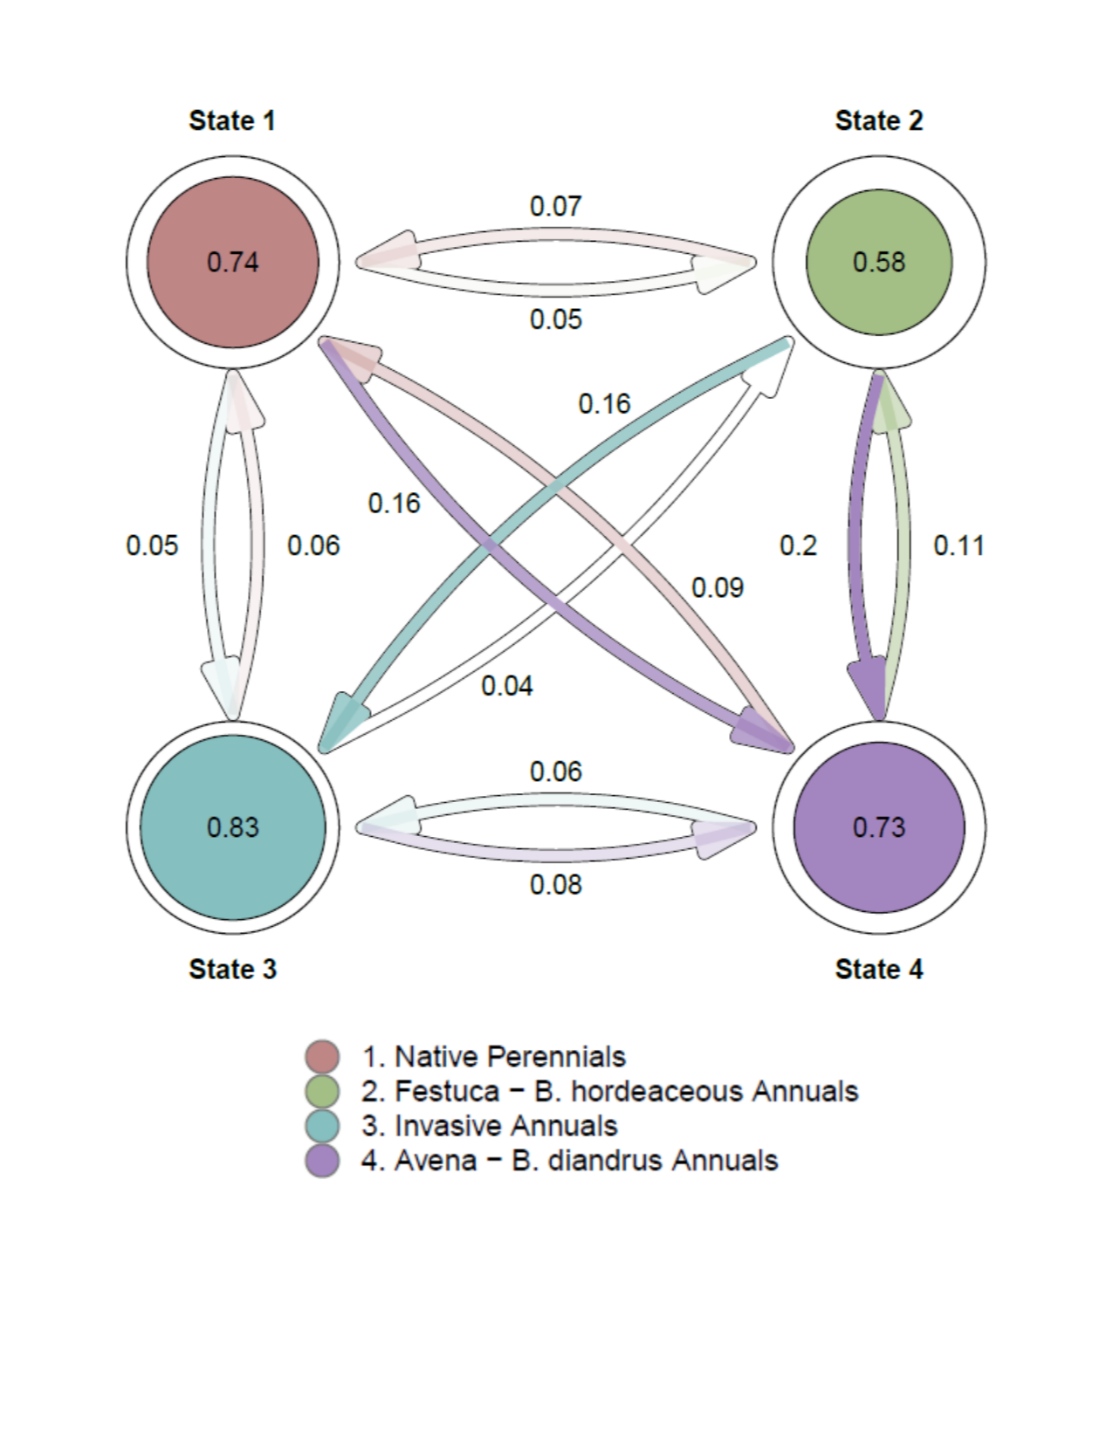
\includegraphics[width=1\textwidth,height=0.8\textheight]{figure/Fig3_3.png}
\caption{State-transition representation of fitted multi-state model coefficients at baseline, assuming no effects of temporal priority and average drought stress (SPEI = 0). Labels refer to the probability a plot transitions between 2 different state assignments (arrows) or the probability a plot retains its assignment (circles) in consecutive years. Circles and arrows are scaled in diameter or color, respectively, by the probability of state assignment transition. \label{fig-3-3}}
\end{figure}
State resistance, the probability of a community changing its state assignment in a subsequent year, varied significantly across the four vegetation types.
Baseline transition matrix values in our model, which assume drought stress equivalent to the long-term average (i.e.~SPEI = 0) and no effects of temporal priority, estimated that the Festuca-B.hordeaceus state was more likely to undergo transition than any of the other state types (Figure 3, Table 2).
Whether driven by competitive differences or interannual feedbacks, the short-term predominance of this community type may be the result of an inherent lack of resistance to colonization by other species groups.

Invasive Annual and Avena-B. diandrus vegetation states that characterized most plant communities exhibited contrasting relationships with drought stress (SPEI; Table 2).
Estimated transition probabilities from the Invasive Annual state were negatively correlated with drought stress (SPEI hazard ratio \textless{} 1), indicating increased state stability when precipitation is above average.
Avena-B. diandrus communities, on the other hand, were estimated to arise more frequently from the Invasive Annual state and maintain this configuration with greater probability under drought (SPEI hazard ratio \textgreater{} 1).
These state-specific responses to water availability appears likely to mediate long-term patterns of vegetation turnover between these community types, though our inference is limited by available data on observed community trajectories post-drought.
\begin{table}[ht]
\centering
\begin{tabular}{lllll}
  \hline
Assignment & Transition & Probability & Temporal Priority & Drought Stress (SPEI) \\ 
  \hline
State 1 & State 1 & 0.74 (0.65,0.8) & - & - \\ 
  State 1 & State 2 & 0.05 (0.03,0.08) & 4.77\verb|^| & 0.8 \\ 
  State 1 & State 3 & 0.05 (0.03,0.1) & 2.96 & 0.95 \\ 
  State 1 & State 4 & 0.16 (0.11,0.23) & 1.53 & 0.86 \\ 
  State 2 & State 1 & 0.07 (0.04,0.11) & 3.31\verb|^| & 0.83 \\ 
  State 2 & State 2 & 0.58 (0.48,0.65) & - & - \\ 
  State 2 & State 3 & 0.16 (0.11,0.23) & 1.71 & 1.41 \\ 
  State 2 & State 4 & 0.2 (0.14,0.27) & 0.54 & 0.71 \\ 
  State 3 & State 1 & 0.06 (0.03,0.11) & 12.74** & 0.56* \\ 
  State 3 & State 2 & 0.04 (0.02,0.07) & 0.55 & 0.55\verb|^| \\ 
  State 3 & State 3 & 0.83 (0.75,0.88) & - & - \\ 
  State 3 & State 4 & 0.08 (0.05,0.12) & 3.26* & 0.56* \\ 
  State 4 & State 1 & 0.09 (0.06,0.15) & 2.53* & 1.43* \\ 
  State 4 & State 2 & 0.11 (0.08,0.17) & 0.77 & 1.02 \\ 
  State 4 & State 3 & 0.06 (0.04,0.11) & 1.93 & 0.98 \\ 
  State 4 & State 4 & 0.73 (0.65,0.79) & - & - \\ 
   \hline
\end{tabular}
\caption{Parameter estimates of the best fit multi-state model (Model 6). For each state assignment, potential state assignments in subsequent years (Transitions) and their associated probabilities (with 95 percent confidence intervals) are reported. Covariate effects reported as hazard ratios, where superscripts correspond to statistical significance: $` = P < 0.1; * = P < 0.05; ** = P < 0.01$} 
\end{table}
In contrast to states which exhibited linearly correlated responses to drought stress, plots characterized by the Native Perennial state displayed complex interactions between effects of drought stress and initial planting composition (Figure 4, Table 2).
The probability of community transition to the Native Perennial state significantly increased under both positive and negative values of SPEI, depending on prior configuration; Invasive Annual communities were more likely to transition to a Native Perennial state under drought, while Avena-B. diandrus communities were more likely to do so with increased water availability.
Critically, these transitions were strongly affected by seeding treatments, where plots seeded with native perennial grasses were significantly more likely to transition (Temporal Priority hazard ratios \textgreater{} 1; Table 3).
This finding suggests that Native Perennial species may be broadly tolerant of climatic variation but limited in their capacity to dominate communities when their propagules are not supplemented.
\begin{figure}
\centering
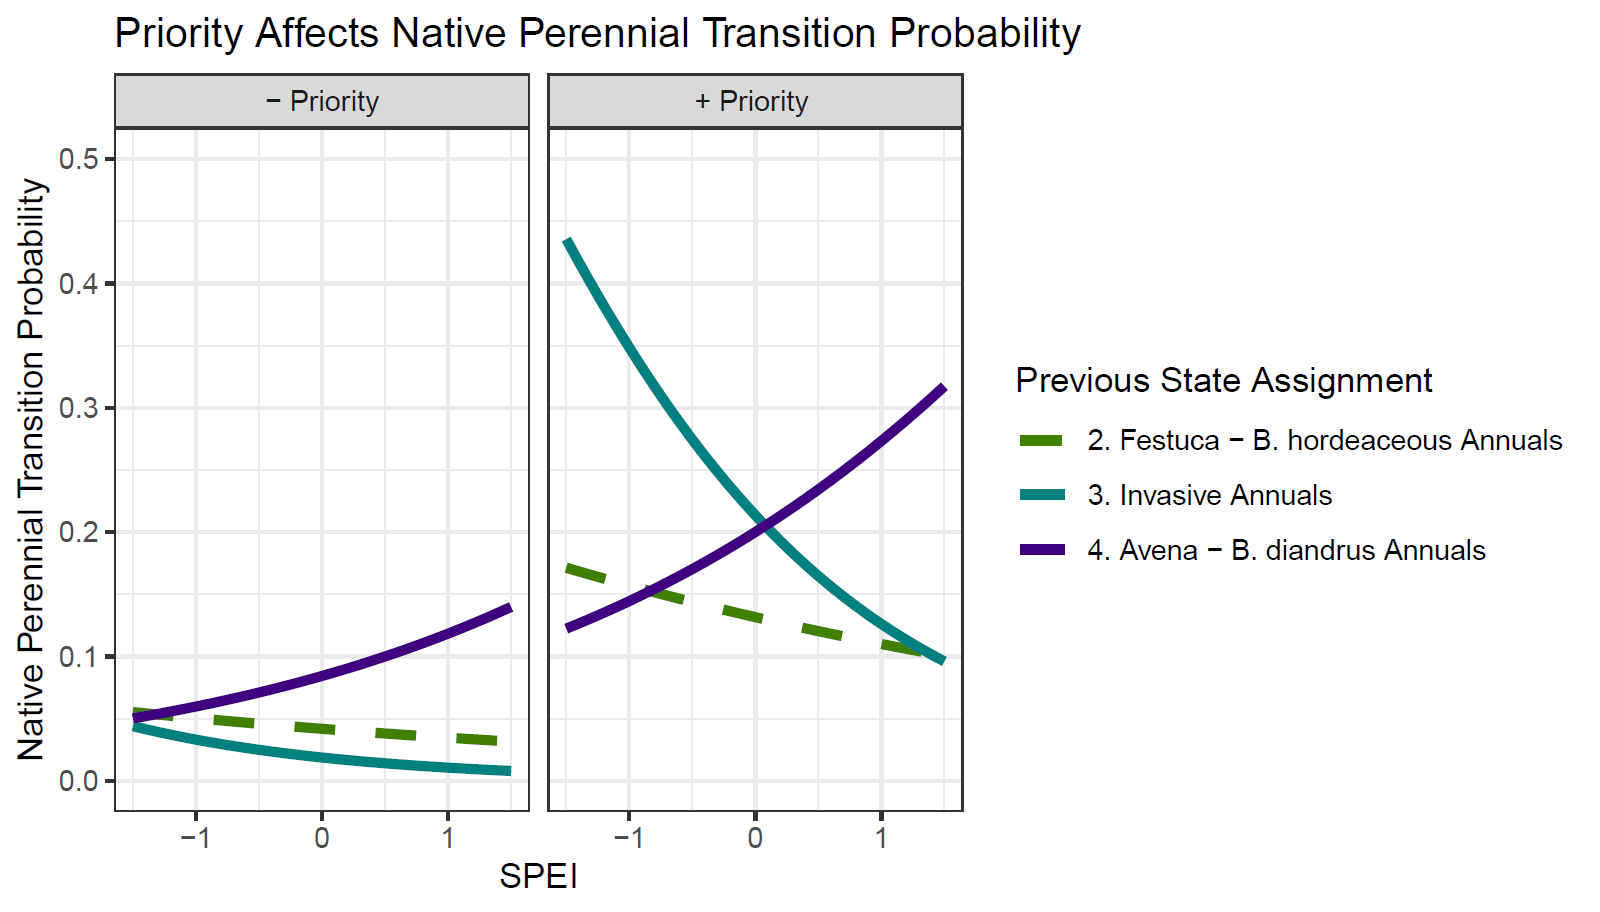
\includegraphics[width=\textwidth,height=0.4\textheight]{figure/Fig3_4.png}
\caption{The effects of temporal priority and drought stress on the probability of transition of a plot to the Native Perennial state given other previous state assignments. Transition probabilities presented are a function of drought stress (SPEI) and whether native species were included/absent from the seeded species mixture (+/- Priority). Solid lines indicate significant (p \textless{} 0.05) covariate effects of both SPEI and priority; dashed lines correspond to non-significant effects. \label{fig-3-4}}
\end{figure}
\hypertarget{discussion}{%
\section{Discussion}\label{discussion}}

\emph{Species response groups under climate extremes}

The emergence of unique community assemblages under climate change is expected to pose a major challenge to the study and management of natural systems in the near future (Hobbs et al. \protect\hyperlink{ref-Hobbs2009}{2009}).
California, like many Mediterranean systems, is projected to experience increasing temperatures and fewer, more extreme rainfall events (Yoon et al. \protect\hyperlink{ref-Yoon2015}{2015}).
Unprecedented climatic extremes will likely produce unintuitive patterns of community assembly that are poorly predicted by prior observations (Williams and Jackson \protect\hyperlink{ref-Williams2007}{2007}); however, contemporary observation of extreme events can shed light onto future dynamics.

In this study, we found evidence that core community assemblages under extreme drought differed from historic norms.
Classic conceptual models that describe vegetation through three discrete state types failed to capture community turnover as effectively as a four-state model that partitioned the traditional ``Naturalized Annual Grasses'' state into two separate groups defined by B. hordeaceous and F. perennis, or A. fatua and B. diandrus.
This result is particularly striking given the structure imposed by our initial planting composition.

While exotic grasses in California are often expected to share similar climatic tolerances due to their annual life history strategy (Sandel and Dangremond \protect\hyperlink{ref-Sandel2012}{2012}), the unique conditions imposed by extreme drought may have crossed previously unobserved thresholds to separate ``winners'' and ``losers'' within functional groups (Prugh et al. \protect\hyperlink{ref-Prugh2018}{2018}).
The mechanism of this partitioning is unclear, but it appears likely that extreme events may operate on secondary divisions within the ``Naturalized Annual Grass'' group.
B. diandrus, for example, is a more common dominant in Southern California grasslands (Barbour et al. \protect\hyperlink{ref-Barbour2007}{2007}), and may exhibit adaptations that provide a competitive advantage under lower water availability.
In contrast, F. perennis tends to be active later into the dry season, and likely fares poorly in drought.

Our partitioning results highlight the potential difficulty in extending species-environment relationships to unobserved conditions (Nippert et al. \protect\hyperlink{ref-Nippert2006}{2006}).
In semi-arid systems, predictions of ecosystem responses to extreme drought are likely to perform poorly when extrapolated from less extreme events.
Drought severity is defined by a suite of characteristics related to event size, frequency, and soil water content, whose combined effect on vegetation may not scale linearly with an aggregate measure of drought stress (Fay et al. \protect\hyperlink{ref-Fay2008}{2008}).
In addition, drought responses of locally interacting species are further controlled by factors such as resource competition, mutualism, and herbivory (Tylianakis et al. \protect\hyperlink{ref-Tylianakis2008}{2008}, Suttle et al. \protect\hyperlink{ref-Suttle2007}{2007}).
In some cases, these complex interactions under novel climate conditions may produce nonlinear relationships or unintuitive mechanisms of change (Stuble et al. \protect\hyperlink{ref-Stuble2017}{2017}).
Warmer temperatures and decreased rainfall has been observed to favor cold-adapted species in the Chihuahuan desert (Kimball et al. \protect\hyperlink{ref-Kimball2010}{2010}), for example, while species abundances following an extreme drought in Switzerland were best predicted by seed production in a system formerly governed by competitive outcomes (Stampfli and Zeiter \protect\hyperlink{ref-Stampfli2004}{2004}).

As these results collectively demonstrate, refinement of conceptual ecosystem models following extreme events may increase their utility under future climate conditions.
Our findings underscore the need for analytical approaches able to critically evaluate these conceptual tools.
Particularly in rangeland systems, which decompose community dynamics into fluctuations between species groups, clustering approaches may effectively capture the novel, site-specific community assemblages that are likely to arise under climate change.

\emph{Contingency in vegetation dynamics}

In this study, we found that species turnover in California grasslands is contingent on both climatic variation and prior patterns of community assembly.
Early abundance of the Festuca-B. hordeaceous state gave rise to communities dominated by Invasive Annual species under above-average precipitation.
Under drought, however, many of these communities failed to return to this initial state type, instead transitioning to the Avena-B. diandrus state.
Transitions to a fourth state, Native Perennials, increased under both drought and water surplus, but depended strongly on a community's prior state type and experimental seed addition.

These state-specific patterns of change are likely driven by variation in the dominant species which characterize each state.
Dominant species are often observed to be primary determinants of key community attributes in grassland systems, such as productivity (Smith and Knapp \protect\hyperlink{ref-Smith2003}{2003}), drought tolerance (Hoover et al. \protect\hyperlink{ref-Hoover2014}{2014}), and resistance to invasion (Smith et al. \protect\hyperlink{ref-Smith2004}{2004}).
And like other studies of California grassland dynamics in a state-transition perspective (Jackson and Bartolome \protect\hyperlink{ref-Jackson2002}{2002}\protect\hyperlink{ref-Jackson2002}{b}, Stein et al. \protect\hyperlink{ref-Stein2016}{2016}), the species that define our vegetation states may be linked to a number of potential mechanisms that influence community turnover.

Across the four vegetation groups we identified, known species characteristics related to competitor inhibition and recruitment appear correlated with observed persistence and transition probabilities, respectively.
Invasive annual grasses, A. triuncialis and E. caput-medusae, facilitate their persistence through deposition of dense thatch layers that inhibit germination and growth of competitors (Eviner and Hawkes \protect\hyperlink{ref-Eviner2012}{2012}).
While native perennial grasses are effective competitors once mature, increased transition probabilities following experiment seeding likely reflects recruitment limitation that is thought to limit colonization {[}Seabloom et al. (\protect\hyperlink{ref-Seabloom2003a}{2003}\protect\hyperlink{ref-Seabloom2003a}{b}); Seabloom2003b{]}.
This contrasts with many naturalized annual grasses, whose large investment into seed production may facilitate rapid colonization and contribute to positive nutrient cycling feedbacks (Eviner and Hawkes \protect\hyperlink{ref-Eviner2012}{2012}, Hillerislambers et al. \protect\hyperlink{ref-Hillerislambers2010}{2010}).

While climate variation may favor certain species groups in isolation, the pathways of community change we observed suggest that climatic effects interact strongly with other state properties -- rather than exhibiting a consistent relationship with precipitation, state frequencies in a given year depended on both climate conditions and state frequencies in years prior.
Though limited to short-term recovery, our findings indicate that state persistence and variable susceptibility to community change may help explain lagged recovery or a failure to return to previous ecosystem states following drought (Smith et al. \protect\hyperlink{ref-Smith2015}{2015}).
Compositional changes following climate events can produce long-lasting effects on successional trajectories, where post-drought species assemblages exhibit strong persistence or altered pathways of community change (Kreyling et al. \protect\hyperlink{ref-Kreyling2011}{2011}).
Other studies of drought effects in California grasslands show similar trends, in which community recovery lags behind climate trends (Harrison et al. \protect\hyperlink{ref-Harrison2018}{2018}); or exhibits selective pathways of change, where return to only a subset of initial state types is possible (Larios et al. \protect\hyperlink{ref-Larios2013}{2013}).

\emph{Implications for Restoration and Management}

While drought is often linked to a number of negative ecosystem changes, such as reduced biodiversity and invasive species spread, the novel conditions imposed by extreme climatic events may also facilitate management efforts (Hobbs et al. \protect\hyperlink{ref-Hobbs2006}{2006}, \protect\hyperlink{ref-Hobbs2009}{2009}, Seastedt et al. \protect\hyperlink{ref-Seastedt2008}{2008}).
By quantifying the persistence of species assemblages under various contexts, our results provide a foundation to better predict windows of opportunity and design effective interventions.
The establishment of native perennial grasses is a common restoration target in California annual grasslands, though success is limited and highly contingent on year-to-year variation (Stromberg et al. \protect\hyperlink{ref-Stromberg2007}{2007}, Young et al. \protect\hyperlink{ref-Young2014}{2014}).
Many restoration efforts in this system utilize temporal or spatial priority to manipulate competitive relationships during planting, in the hope that early establishment delays or prevents encroachment by less desirable species (Wainwright et al. \protect\hyperlink{ref-Wainwright2012}{2012}, Fry et al. \protect\hyperlink{ref-Fry2017}{2017}, Young et al. \protect\hyperlink{ref-Young2017}{2017}).
For native perennial grasses in California annual grasslands, we found strong evidence that priority seeding can assist in establishing and maintaining a desired community that remains relatively persistent after planting or provide the basis for subsequent dominance when conditions are favorable (Porensky et al. \protect\hyperlink{ref-Porensky2012}{2012}).

In contrast, our study suggests that eradication of invasive annual grasses may be facilitated by targeted management during drought.
Common interventions--grazing, herbicide application, and targeted burning--may be more effective when conditions naturally disadvantage E. caput-medusae and A. triucialis (DiTomaso et al. \protect\hyperlink{ref-DiTomaso2008}{2008}).
However, given that vegetation states may vary in persistence, managers must take care to ensure that colonizing vegetation is robust to re-invasion.
Growth of ruderal weeds appears common following management in California grasslands, which often do little to resist colonization of invasive grasses (Young \protect\hyperlink{ref-Young1992}{1992}, DiTomaso et al. \protect\hyperlink{ref-DiTomaso2008}{2008}).

Generally, our findings underscore the potential value of maintaining functional and taxonomic diversity in restoration and management (Funk et al. \protect\hyperlink{ref-Funk2008}{2008}) .
Particularly in highly dynamic systems where environmental fluctuations drive turnover, long-term ecosystem health may depend on turnover among desirable community types--the maintenance of multiple potential vegetation states can maintain favorable pathways of compositional change following disturbance that may otherwise favor spread of undesirable species (Hoover et al. \protect\hyperlink{ref-Hoover2014}{2014}, Griffin-Nolan et al. \protect\hyperlink{ref-Griffin-Nolan2019}{2019}, Wilcox et al. \protect\hyperlink{ref-Wilcox2020}{2020}).

\emph{Future Directions}

This study highlights the need to employ analytical approaches capable of distinguishing novel assemblages as they arise.
Reliance on long-standing divisions between species groups to characterize system responses to climate change may fail to capture emergent complexity.
However, while we were able to capture the immediate effects of a historic drought on grassland plant communities, the scope of our study is focused on a relatively narrow time period that may be insufficient to capture long-term changes to vegetation dynamics.
Continued observation, particularly over a broader range of climatic conditions, may further refine partitions between core species groups and better capture ecosystem recovery to extreme events.

\hypertarget{conclusion}{%
\chapter*{Conclusion}\label{conclusion}}
\addcontentsline{toc}{chapter}{Conclusion}

If we don't want Conclusion to have a chapter number next to it, we can add the \texttt{\{-\}} attribute.

\textbf{More info}

And here's some other random info: the first paragraph after a chapter title or section head \emph{shouldn't be} indented, because indents are to tell the reader that you're starting a new paragraph. Since that's obvious after a chapter or section title, proper typesetting doesn't add an indent there.

\appendix

\hypertarget{chapter-1-supporting-information}{%
\chapter{Chapter 1 Supporting Information}\label{chapter-1-supporting-information}}
\begin{table}[ht]
\centering
\scalebox{0.6}{
\begin{tabular}{llllllllll}
  \hline
Site Name & Continent & Country & Habitat & First Year & Last Year & Total Years & MAP & MAT & Taxa \\ 
  \hline
Azi & Asia & CN & alpine grassland & 2007 & 2012 & 5 & 711 & 1.36 & 43 \\ 
  Bogong & Australia & AU & alpine grassland & 2009 & 2019 & 11 & 1678 & 5.98 & 19 \\ 
  Boulder South Campus & North America & US & shortgrass prairie & 2008 & 2016 & 9 & 487 & 9.9 & 9 \\ 
  Bunchgrass (Andrews LTER) & North America & US & montane grassland & 2007 & 2018 & 12 & 1618 & 6.77 & 10 \\ 
  Burrawan & Australia & AU & semiarid grassland & 2008 & 2019 & 12 & 643 & 18.22 & 10 \\ 
  Cedar Creek LTER & North America & US & tallgrass prairie & 2007 & 2018 & 12 & 740 & 6.34 & 8 \\ 
  Cedar Point Biological Station & North America & US & shortgrass prairie & 2007 & 2019 & 13 & 456 & 9.64 & 12 \\ 
  CEREEP - Ecotron IDF & Europe & FR & old field & 2012 & 2018 & 7 & 632 & 10.82 & 16 \\ 
  Chichaqua Bottoms & North America & US & tallgrass prairie & 2009 & 2019 & 11 & 871 & 9.26 & 6 \\ 
  Companhia das Lezirias & Europe & PT & annual grassland & 2012 & 2019 & 8 & 564 & 16.58 & 26 \\ 
  Cowichan & North America & CA & old field & 2007 & 2018 & 12 & 762 & 10.45 & 5 \\ 
  Elliott Chaparral & North America & US & annual grassland & 2008 & 2019 & 11 & 344 & 17.71 & 6 \\ 
  Ethabuka (Main Camp) & Australia & AU & desert grassland & 2013 & 2019 & 7 & 192 & 24.06 & 4 \\ 
  Ethabuka (South Site) & Australia & AU & desert grassland & 2013 & 2019 & 7 & 203 & 23.95 & 3 \\ 
  Fruebuel & Europe & CH & pasture & 2008 & 2015 & 8 & 1546 & 6.96 & 15 \\ 
  Hall's Prairie & North America & US & tallgrass prairie & 2007 & 2014 & 8 & 1289 & 13.83 & 4 \\ 
  Hart Mountain & North America & US & shrub steppe & 2007 & 2012 & 6 & 259 & 7.75 & 11 \\ 
  Heronsbrook (Silwood Park) & Europe & UK & mesic grassland & 2007 & 2013 & 7 & 668 & 10.17 & 19 \\ 
  Hopland REC & North America & US & annual grassland & 2007 & 2019 & 13 & 1065 & 13.24 & 19 \\ 
  Jena & Europe & DE & grassland & 2013 & 2018 & 6 & 654 & 8.57 & 18 \\ 
  Kibber (Spiti) & Asia & IN & alpine grassland & 2011 & 2018 & 8 & 400 & -1.45 & 7 \\ 
  Kilpisjärvi & Europe & FI & tundra grassland & 2013 & 2018 & 6 & 569 & -3.25 & 24 \\ 
  Kinypanial & Australia & AU & semiarid grassland & 2007 & 2018 & 11 & 408 & 15.59 & 8 \\ 
  Koffler Scientific Reserve & North America & CA & pasture & 2010 & 2019 & 10 & 853 & 6.28 & 10 \\ 
  Konza LTER & North America & US & tallgrass prairie & 2007 & 2019 & 13 & 889 & 12.08 & 17 \\ 
  Lancaster & Europe & UK & mesic grassland & 2008 & 2017 & 10 & 1522 & 8.01 & 10 \\ 
  Las Chilcas & South America & AR & mesic grassland & 2013 & 2019 & 7 & 955 & 15.09 & 8 \\ 
  Lookout (Andrews LTER) & North America & US & montane grassland & 2007 & 2018 & 12 & 1877 & 6.9 & 8 \\ 
  Mar Chiquita & South America & AR & grassland & 2011 & 2018 & 8 & 907 & 14.32 & 14 \\ 
  Mclaughlin UCNRS & North America & US & annual grassland & 2007 & 2019 & 13 & 936 & 13.97 & 8 \\ 
  Mt. Caroline & Australia & AU & savanna & 2008 & 2018 & 11 & 324 & 17.75 & 15 \\ 
  Pingelly Paddock & Australia & AU & old field & 2013 & 2018 & 6 & 456 & 16.28 & 10 \\ 
  Pinjarra Hills & Australia & AU & pasture & 2013 & 2018 & 5 & 1085 & 19.99 & 5 \\ 
  Rookery (Silwood Park) & Europe & UK & mesic grassland & 2007 & 2013 & 7 & 685 & 10.13 & 12 \\ 
  Saana & Europe & FI & montane grassland & 2014 & 2019 & 6 & 521 & -2.6 & 25 \\ 
  Sagehen Creek UCNRS & North America & US & montane grassland & 2007 & 2013 & 7 & 831 & 5.83 & 16 \\ 
  Savannah River & North America & US & savanna & 2007 & 2012 & 6 & 1184 & 17.43 & 12 \\ 
  Sedgwick Reserve UCNRS & North America & US & annual grassland & 2007 & 2017 & 11 & 478 & 15.58 & 4 \\ 
  Sevilleta LTER & North America & US & desert grassland & 2007 & 2018 & 12 & 252 & 13.06 & 5 \\ 
  Sheep Experimental Station & North America & US & shrub steppe & 2007 & 2016 & 10 & 246 & 5.32 & 18 \\ 
  Shortgrass Steppe LTER & North America & US & shortgrass prairie & 2007 & 2018 & 12 & 369 & 8.95 & 6 \\ 
  Sierra Foothills REC & North America & US & annual grassland & 2007 & 2019 & 13 & 936 & 16.31 & 7 \\ 
  Smith Prairie & North America & US & mesic grassland & 2007 & 2016 & 10 & 605 & 10.18 & 25 \\ 
  Spindletop & North America & US & pasture & 2007 & 2019 & 13 & 1152 & 12.48 & 9 \\ 
  Temple & North America & US & tallgrass prairie & 2007 & 2016 & 10 & 877 & 19.4 & 15 \\ 
  Trelease & North America & US & tallgrass prairie & 2008 & 2017 & 10 & 992 & 11.07 & 5 \\ 
  Ukulinga & Africa & ZA & mesic grassland & 2009 & 2018 & 10 & 832 & 17.65 & 17 \\ 
  Val Mustair & Europe & CH & alpine grassland & 2008 & 2019 & 11 & 681 & 0.13 & 30 \\ 
  Yarramundi & Australia & AU & mesic grassland & 2014 & 2019 & 6 & 844 & 17.32 & 5 \\ 
   \hline
\end{tabular}
}
\caption{Table of sites included in analysis.} 
\end{table}
\begin{table}[ht]
\centering
\scalebox{0.6}{
\begin{tabular}{llllllll}
  \hline
Site Name & $\rho$(N-P) & $\rho$(N-K) & $\rho$(P-K) & $\Delta$N & $\Delta$P & $\Delta$K & D \\ 
  \hline
Azi & 0.4 & 0.68 & 0.47 & 1.3 & 1.35 & 1.44 & 0.32 \\ 
  Bogong & 0.28 & 0.59 & 0.57 & 0.44* & 0.42* & 0.38* & 0.35 \\ 
  Boulder South Campus & -0.06 & 0.05 & 0.67 & 0.44 & 0.56* & 0.44 & 0.52 \\ 
  Bunchgrass (Andrews LTER) & 0.22 & 0.67 & 0.52 & 0.25 & 0.46* & 0.43* & 0.35 \\ 
  Burrawan & 0.26 & 0.32 & -0.03 & 0.17 & 0.2 & 0.17 & 0.54 \\ 
  Cedar Creek LTER & 0.43 & 0.14 & 0.57 & 0.53* & 0.18 & 0.22 & 0.41 \\ 
  Cedar Point Biological Station & 0.2 & 0.18 & 0.43 & 0.36* & 0.23* & 0.27* & 0.49 \\ 
  CEREEP - Ecotron IDF & 0.13 & 0.15 & 0.61 & 1.12* & 0.91 & 1.12* & 0.47 \\ 
  Chichaqua Bottoms & 0.48 & 0.57 & 0.6 & 0.30* & 0.25 & 0.27* & 0.3 \\ 
  Companhia das Lezirias & 0.44 & 0.2 & 0.38 & 1.15* & 1.10* & 0.75 & 0.44 \\ 
  Cowichan & -0.3 & 0.66 & -0.01 & 0.12 & 0.27* & 0.17 & 0.59 \\ 
  Elliott Chaparral & 0.5 & -0.12 & 0.66 & 0.22 & 0.26 & 0.27 & 0.44 \\ 
  Ethabuka (Main Camp) & -0.08 & 0.57 & 0.28 & 0.28 & 0.83* & 0.43 & 0.5 \\ 
  Ethabuka (South Site) & 0.77 & 0.88 & 0.92 & 0.59* & 0.32 & 0.52 & 0.09 \\ 
  Fruebuel & 0.58 & 0.15 & 0.49 & 1.05* & 0.99* & 0.83* & 0.4 \\ 
  Hall's Prairie & 0.56 & 0.58 & 0.04 & 1.13* & 0.66* & 0.68* & 0.4 \\ 
  Hart Mountain & 0.91 & 0.46 & 0.5 & 0.96* & 0.73 & 0.57 & 0.25 \\ 
  Heronsbrook (Silwood Park) & 0.21 & 0.6 & 0.28 & 1.03* & 0.67 & 0.66 & 0.42 \\ 
  Hopland REC & 0.33 & 0.75 & 0.58 & 1.01* & 0.49 & 0.68* & 0.3 \\ 
  Jena & -0.25 & 0.06 & 0.2 & 0.97* & 0.62 & 0.64 & 0.67 \\ 
  Kibber (Spiti) & 0.3 & 0.48 & 0.74 & 0.25 & 0.26 & 0.27 & 0.33 \\ 
  Kilpisjärvi & 0.4 & 0.22 & 0.8 & 1.03* & 0.78 & 0.46 & 0.35 \\ 
  Kinypanial & -0.08 & 0.23 & 0.84 & 0.16 & 0.32 & 0.26 & 0.45 \\ 
  Koffler Scientific Reserve at Joker's Hill & 0.32 & 0.6 & 0.53 & 0.88* & 0.65* & 0.54* & 0.34 \\ 
  Konza LTER & 0.29 & 0.23 & 0.55 & 0.43* & 0.28 & 0.37 & 0.43 \\ 
  Lancaster & 0.55 & 0.57 & 0.57 & 0.44 & 0.38 & 0.38 & 0.29 \\ 
  Las Chilcas & 0.71 & 0.55 & 0.83 & 0.78* & 0.52 & 0.84* & 0.2 \\ 
  Lookout (Andrews LTER) & 0.66 & 0.88 & 0.86 & 0.38* & 0.39* & 0.50* & 0.13 \\ 
  Mar Chiquita & 0.75 & 0.54 & 0.6 & 0.62 & 0.58 & 0.6 & 0.25 \\ 
  Mclaughlin UCNRS & 0.51 & 0.24 & 0.24 & 0.41 & 0.33 & 0.38 & 0.45 \\ 
  Mt. Caroline & 0.67 & 0.71 & 0.6 & 0.67* & 0.62* & 0.52* & 0.23 \\ 
  Pingelly Paddock & 0.46 & -0.08 & -0.29 & 0.74 & 1.28* & 0.61 & 0.65 \\ 
  Pinjarra Hills & 0.55 & 0.25 & 0.81 & 0.78 & 1.06 & 0.77 & 0.31 \\ 
  Rookery (Silwood Park) & 0.8 & 0.74 & 0.8 & 0.99* & 1.50* & 0.73 & 0.15 \\ 
  Saana & 0.61 & 0.56 & 0.62 & 1.25* & 0.98* & 1.09* & 0.27 \\ 
  Sagehen Creek UCNRS & 0.12 & 0.49 & 0.17 & 0.63 & 0.49 & 0.45 & 0.49 \\ 
  Savannah River & 0.42 & 0.12 & 0.38 & 0.76 & 0.99 & 0.55 & 0.46 \\ 
  Sedgwick Reserve UCNRS & 0.61 & 0.84 & 0.94 & 0.38* & 0.39* & 0.36* & 0.14 \\ 
  Sevilleta LTER & 0.8 & 0.92 & 0.94 & 0.36* & 0.14 & 0.14 & 0.08 \\ 
  Sheep Experimental Station & -0.11 & 0.53 & -0.12 & 0.28* & 0.17 & 0.21 & 0.6 \\ 
  Shortgrass Steppe LTER & -0.01 & 0.36 & 0.53 & 0.43* & 0.26* & 0.1 & 0.47 \\ 
  Sierra Foothills REC & -0.38 & 0.23 & 0.59 & 0.34 & 0.24 & 0.29 & 0.57 \\ 
  Smith Prairie & 0.15 & 0.15 & 0.06 & 0.53* & 0.47* & 0.35 & 0.59 \\ 
  Spindletop & 0.66 & 0.14 & 0.2 & 0.24 & 0.25 & 0.60* & 0.44 \\ 
  Temple & 0.28 & 0.24 & 0.5 & 0.41 & 0.61* & 0.55 & 0.44 \\ 
  Trelease & -0.27 & -0.51 & 0.48 & 0.55* & 0.28 & 0.23 & 0.73 \\ 
  Ukulinga & 0.17 & -0.06 & 0.51 & 0.58* & 0.51* & 0.75* & 0.53 \\ 
  Val Mustair & 0.56 & 0.4 & 0.45 & 0.45* & 0.57* & 0.3 & 0.35 \\ 
  Yarramundi & 0.75 & 0.65 & 0.2 & 0.36 & 0.36 & 0.65* & 0.31 \\ 
   \hline
\end{tabular}
}
\caption{Table of sites, pairwise correlations between community responses to different treatments ($\rho$), rate of community change in response to treatment ($\Delta$), and estimated response dimensionality (D). Significant (P < 0.05) magnitudes of community response are labelled with *.} 
\end{table}
\begin{figure}
\centering
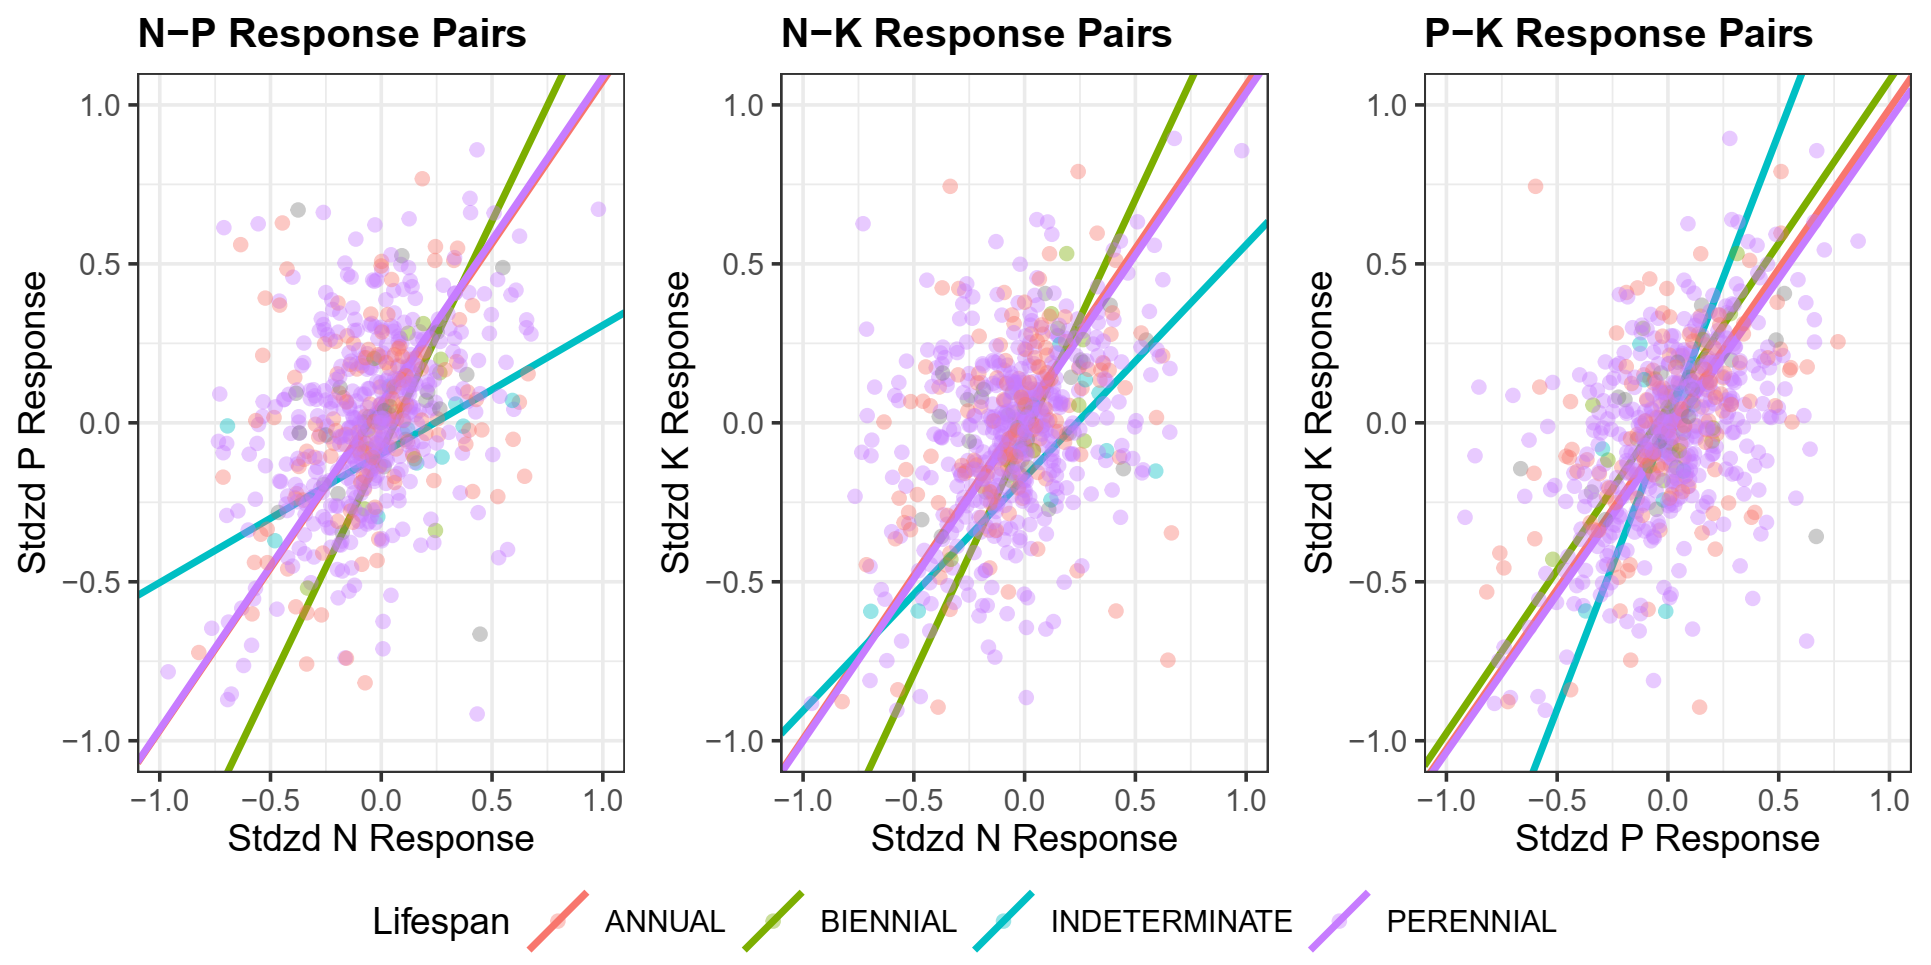
\includegraphics[width=\textwidth,height=0.4\textheight]{figure/AppFig1_1.png}
\caption{Bivariate relationships between treatments colored by species lifespan. \label{app-1-1}}
\end{figure}
\begin{figure}
\centering
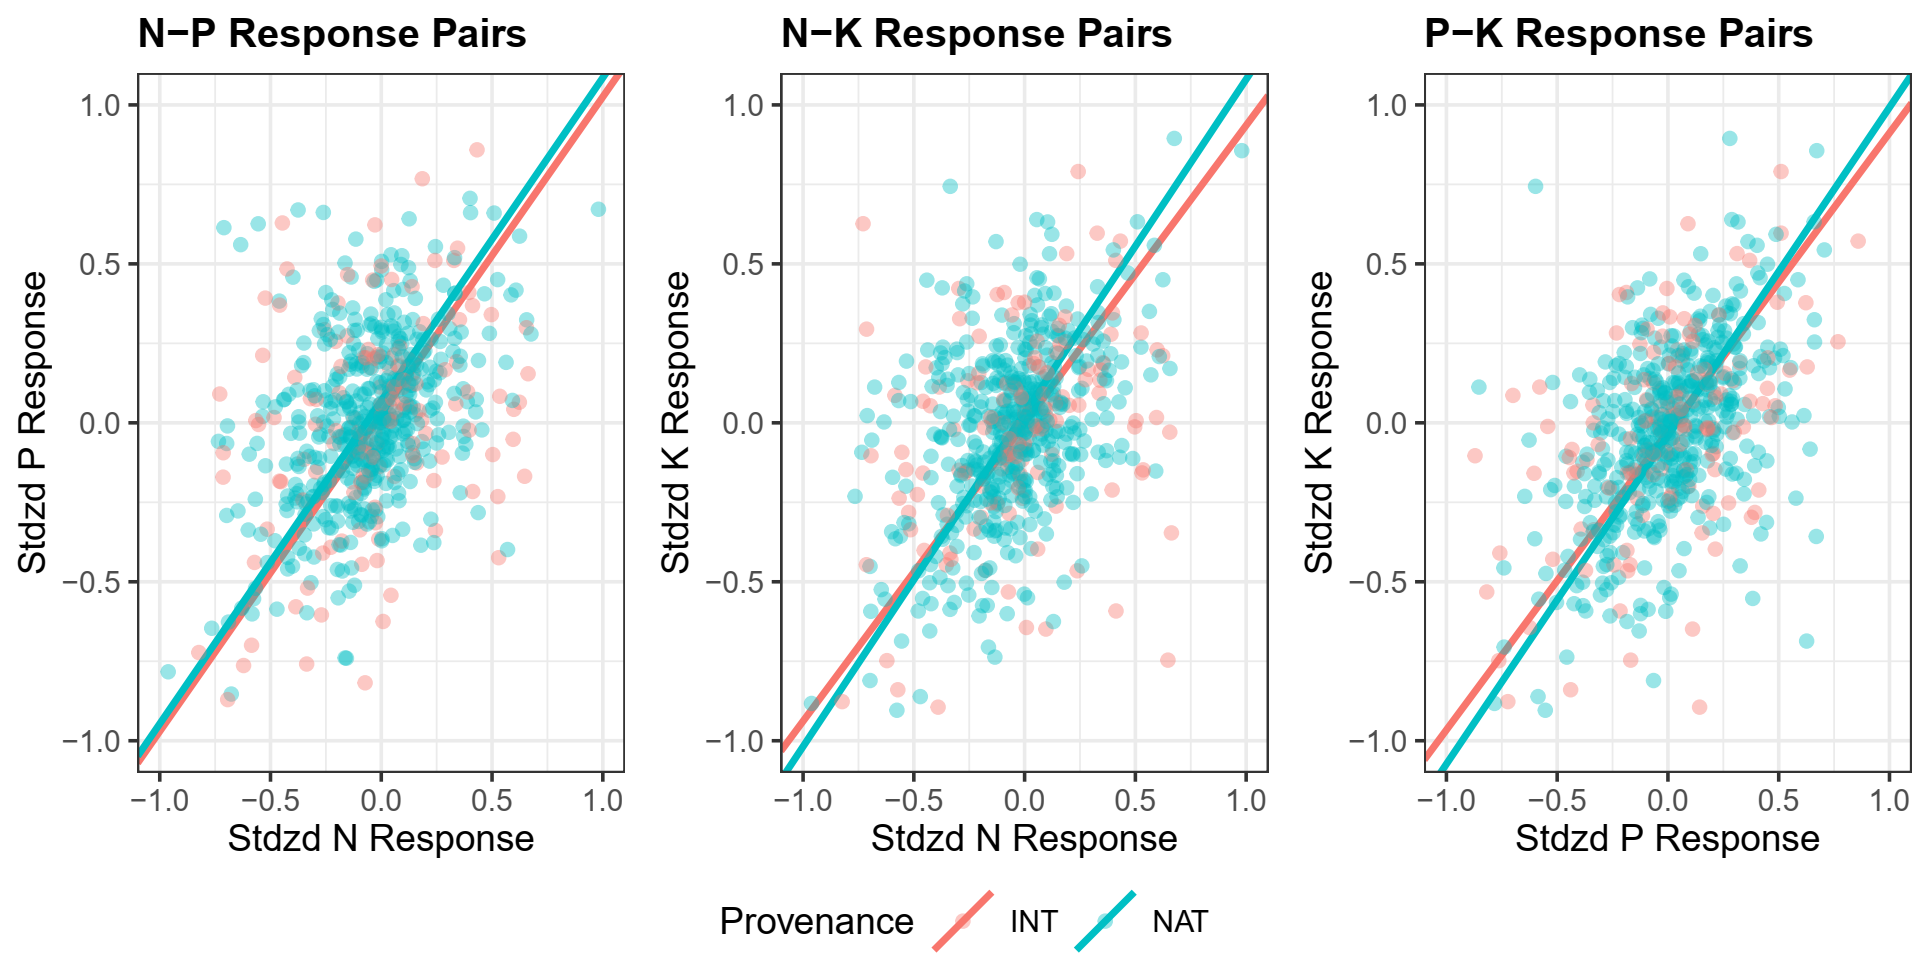
\includegraphics[width=\textwidth,height=0.4\textheight]{figure/AppFig1_2.png}
\caption{Bivariate relationships between treatments colored by provenance (introduced / native). \label{app-1-2}}
\end{figure}
\hypertarget{chapter-2-supporting-information}{%
\chapter{Chapter 2 Supporting Information}\label{chapter-2-supporting-information}}

\hypertarget{chapter-3-supporting-information}{%
\chapter{Chapter 3 Supporting Information}\label{chapter-3-supporting-information}}
\begin{table}[ht]
\centering
\begin{tabular}{lllllll}
  \hline
Source & DF & SS & MS & F & R-squared & P \\ 
  \hline
Seeding composition & 6 & 12.0487 & 2.0081 & 32.815 & 0.8 & 0.001 \\ 
  Residual & 49 & 2.9986 & 0.19928 &   &   &   \\ 
  Total & 55 & 15.0473 & 1 &   &   &   \\ 
   \hline
\end{tabular}
\caption{Heuristics used to determine best number of clusters to use in partitioning, K. Summary of the best performing K for 8 different clustering indices.} 
\end{table}
\begin{table}[ht]
\centering
\scalebox{0.7}{
\begin{tabular}{lllllllllllllllll}
  \hline
K & Hartigan & Rk & CH & Rk & Beale & Rk & KL & Rk & Cindex & Rk & DB & Rk & Sil. & Rk & Duda & Rk \\ 
  \hline
2 & 133.88 & 9 & 163.1 & 3 & 2.7 & 8 & 1.22 & 5 & 0.5 & 9 & 1.69 & 9 & 0.21 & 9 & 0.82 & 9 \\ 
  3 & 128.56 & 5 & 166.15 & 2 & 1.96 & 7 & 1.12 & 6 & 0.45 & 8 & 1.59 & 8 & 0.23 & 8 & 0.86 & 7 \\ 
  4 & 52.25 & 1 & 176.75 & 1 & -2.02 & 1 & 3.09 & 2 & 0.42 & 7 & 1.49 & 6 & 0.26 & 7 & 1.19 & 1 \\ 
  5 & 70 & 7 & 156.78 & 5 & 5.41 & 9 & 0.7 & 8 & 0.4 & 6 & 1.42 & 3 & 0.27 & 6 & 0.7 & 8 \\ 
  6 & 84.36 & 6 & 153.65 & 6 & -2.03 & 2 & 0.87 & 7 & 0.36 & 4 & 1.48 & 5 & 0.3 & 2 & 1.2 & 3 \\ 
  7 & 28.88 & 2 & 159.7 & 4 & 1.12 & 6 & 3.83 & 1 & 0.36 & 5 & 1.4 & 1 & 0.3 & 1 & 0.92 & 6 \\ 
  8 & 63.54 & 8 & 147.31 & 9 & -3.12 & 3 & 0.39 & 9 & 0.31 & 1 & 1.5 & 7 & 0.27 & 5 & 1.34 & 4 \\ 
  9 & 48.78 & 4 & 150.17 & 7 & -2.06 & 5 & 1.42 & 4 & 0.33 & 3 & 1.47 & 4 & 0.29 & 3 & 1.2 & 5 \\ 
  10 & 25.57 & 3 & 149.47 & 8 & -9.33 & 4 & 2.24 & 3 & 0.32 & 2 & 1.42 & 2 & 0.28 & 4 & 4.2 & 2 \\ 
   \hline
\end{tabular}
}
\caption{Rank summary table of performance across different clustering indices.} 
\end{table}
\pagebreak

Clustering Index Ranking Method:
\begin{enumerate}
\def\labelenumi{\arabic{enumi}.}
\tightlist
\item
  Hartigan: Choose value K with maximum index difference between K and K-1.
\item
  CH: Choose maximum value among orders of K considered.
\item
  Beale: Choose minimum value of K such that the critical value of the index is less than alpha = 0.05. Other values whose critical value is less than alpha are ranked in order of significance.
\item
  KL: Choose maximum value among orders of K considered.
\item
  Cindex: Choose minimum value among orders of K considered.
\item
  DB (Davies and Bouldin): Choose minimum value among orders of K considered.
\item
  Silhouette: Choose maximum value among orders of K considered.
\item
  Duda: Choose minimum value of K such that the critical value of the index is less than alpha = 0.05. Other values whose critical value is less than alpha are ranked in order of significance.
\end{enumerate}
\pagebreak
\begin{table}[ht]
\centering
\scalebox{0.7}{
\begin{tabular}{lllll}
  \hline
  & Native perennial & F. perennis - B.hordeaceous & Invasive Annual & A. fatua - B. diandrus \\ 
  \hline
Native perennial & 95 & 8 & 7 & 29 \\ 
  F. perennis - B.hordeaceous & 10 & 50 & 30 & 29 \\ 
  Invasive Annual & 25 & 11 & 115 & 22 \\ 
  A. fatua - B. diandrus & 19 & 21 & 7 & 76 \\ 
   \hline
\end{tabular}
}
\caption{Contingency table of observed transitions between state assignments between 2008-2018. For each plot observation of a state assignment in year t (rows), data shows the frequency of state assignments (columns) of the same plot in a subsequent year (t + 1). Diagonal values represent the frequency of a given state retaining its assignment (persistence), while off-diagonal values represent transitions in state assignment. Changes in assignment frequency were highly non-random ($\chi^2$ = 392.017, df = 9, P < 0.001).} 
\end{table}
\begin{table}[ht]
\centering
\begin{tabular}{llllllrr}
  \hline
Model & DF & Priority & 1 Year SPEI & 2 Year SPEI & 3 Year SPEI & deltaAIC & AIC \\ 
  \hline
1 & 12 &  &  &  &  & 35.31 & 1289.98 \\ 
  2 & 24 & X &  &  &  & 6.16 & 1260.83 \\ 
  3 & 24 &  & X &  &  & 31.82 & 1286.49 \\ 
  4 & 24 &  &  & X &  & 31.76 & 1286.43 \\ 
  5 & 24 &  &  &  & X & 28.00 & 1282.67 \\ 
  6 & 36 & X & X &  &  & 0.00 & 1254.67 \\ 
  7 & 36 & X &  & X &  & 3.92 & 1258.59 \\ 
  8 & 36 & X &  &  & X & 0.25 & 1254.92 \\ 
   \hline
\end{tabular}
\caption{AIC model comparison used to select the best fit multi-state model from a series of candidates. Covariates include “Priority Effects” – the effect of initial seeding mixture representation of indicator species correlated with cluster assignments – and “1-“, “2-“, and “3-year SPEI” – a standardized measure of drought stress computed over 1, 2, and 3 cumulative water year intervals, respectively. DF corresponds to the number of parameters estimated within the transition matrix, including baseline transition probabilities and effects of covariates.} 
\end{table}
\begin{figure}
\centering
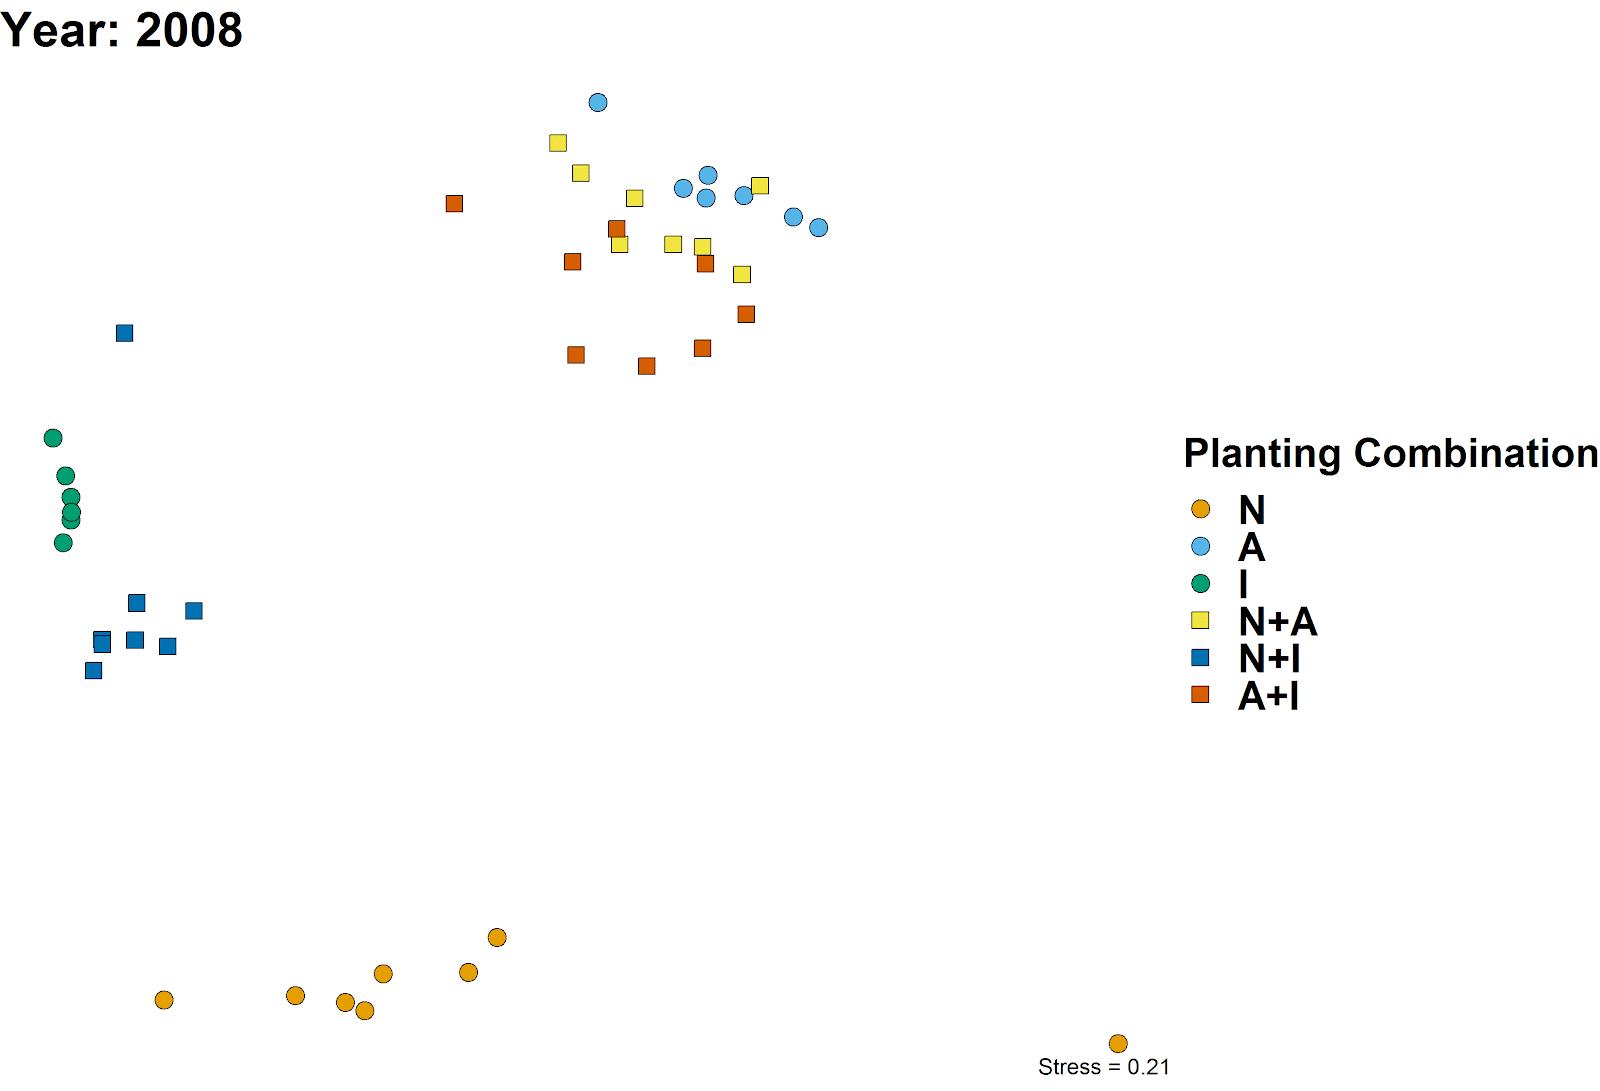
\includegraphics[width=\textwidth,height=0.5\textheight]{figure/AppFig3_1.png}
\caption{Visualization of clustering assignments following K-medoids clustering. Non-metric multidimensional scaling (NMDS) ordination was conducted on all community observations from 2008 -- 2018 (n=560). Pairwise community distance was calculated using Bray-Curtis dissimilarity index. Species vectors correspond to taxa that were found to be significantly associated (p \textless{} 0.05) with state assignments using indicator species analysis. \label{app-3-1}}
\end{figure}
\begin{figure}
\centering
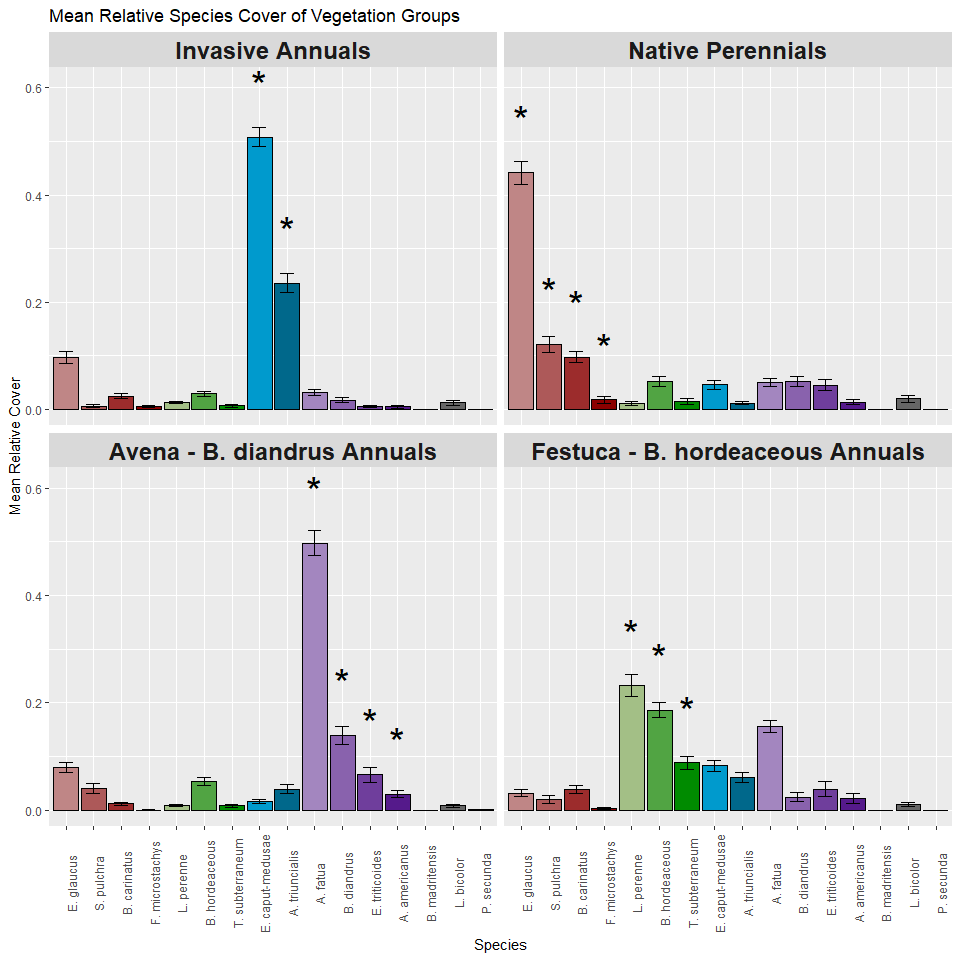
\includegraphics[width=\textwidth,height=0.8\textheight]{figure/AppFig3_2.png}
\caption{Relative abundance of species across vegetation state assignments. Values refer to the average abundance of each species (+/- standard error) for observed communities assigned to each state. Species that served as significant (P \textless{} 0.05) indicators of each state type are highlighted using ``*'' and colored by representative state. On average, indicator species of each vegetation state accounted for 75\% of the cumulative relative abundance of observed communities. \label{app-3-2}}
\end{figure}
\begin{figure}
\centering
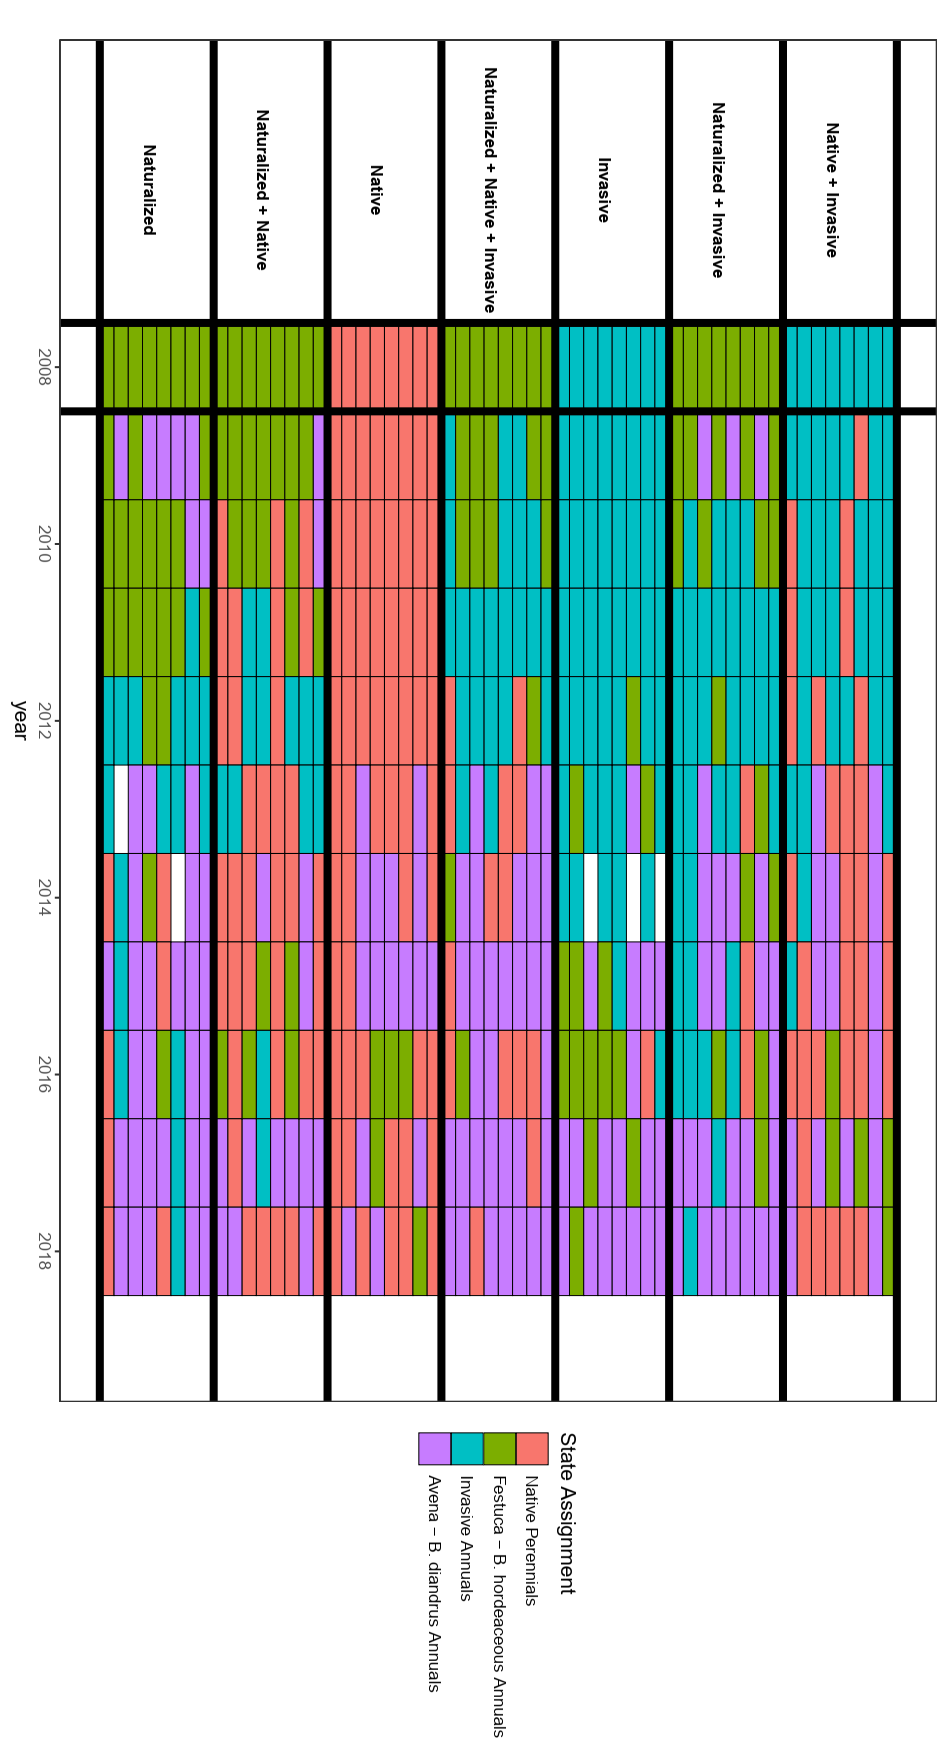
\includegraphics[width=0.65\textwidth,height=0.8\textheight]{figure/AppFig3_3.png}
\caption{Plot-level shifts in state assignment over time. For each observed community (grid cell), the state assignment of a community is presented as a function of initial seeding treatment (row) and time (column). \label{app-3-3}}
\end{figure}
\backmatter

\hypertarget{references}{%
\chapter*{References}\label{references}}
\addcontentsline{toc}{chapter}{References}

\markboth{References}{References}

\noindent

\setlength{\parindent}{-0.20in}
\setlength{\leftskip}{0.20in}
\setlength{\parskip}{8pt}

\hypertarget{refs}{}
\leavevmode\hypertarget{ref-Adler2006}{}%
Adler, P. B., J. HilleRisLambers, P. C. Kyriakidis, Q. Guan, and J. M. Levine. 2006. Climate variability has a stabilizing effect on the coexistence of prairie grasses. Proceedings of the National Academy of Sciences of the United States of America 103:12793--12798.

\leavevmode\hypertarget{ref-Alexander2015}{}%
Alexander, J. M., J. M. Diez, and J. M. Levine. 2015. Novel competitors shape species' responses to climate change. Nature 525:515--518.

\leavevmode\hypertarget{ref-Allen-Diaz1998}{}%
Allen-Diaz, B., and J. W. Bartolome. 1998. Sagebrush -- Grass Vegetation Dynamics : Comparing Classical and State-Transition Models. Ecological Applications 8:795--804.

\leavevmode\hypertarget{ref-Angert2009}{}%
Angert, A. L., T. E. Huxman, P. Chesson, and D. L. Venable. 2009. Functional tradeoffs determine species coexistence via the storage effect. Proceedings of the National Academy of Sciences of the United States of America 106:11641--11645.

\leavevmode\hypertarget{ref-Agren2004}{}%
Ågren, G. I. 2004. The C:N:P stoichiometry of autotrophs - Theory and observations. Ecology Letters 7:185--191.

\leavevmode\hypertarget{ref-Agren2008}{}%
Ågren, G. I. 2008. Stoichiometry and nutrition of plant growth in natural communities. Annual Review of Ecology, Evolution, and Systematics 39:153--170.

\leavevmode\hypertarget{ref-Barbour2007}{}%
Barbour, M. G., T. Keeler-Wolf, and A. A. Schoenherr, editors. 2007. Terrestrial Vegetation of California. University of California Press.

\leavevmode\hypertarget{ref-Bartolome2008}{}%
Bartolome, J. W., B. Allen-Diaz, and R. D. Jackson. 2008. Developing Data-Driven Descriptive Models for Californian Grasslands. Pages 124--135 \emph{in} R. J. Hobbs and K. N. Suding, editors. New models for ecosystem dynamics and restoration. First editions. Island Press, Washington, D.C.

\leavevmode\hypertarget{ref-Begueria2014}{}%
Beguería, S., S. M. Vicente-Serrano, F. Reig, and B. Latorre. 2014. Standardized precipitation evapotranspiration index (SPEI) revisited: Parameter fitting, evapotranspiration models, tools, datasets and drought monitoring. International Journal of Climatology 34:3001--3023.

\leavevmode\hypertarget{ref-Bestelmeyer2003}{}%
Bestelmeyer, B. T., J. R. Brown, K. M. Havstad, R. Alexander, G. Chavez, and J. E. Herrick. 2003. Development and use of state-and-transition models for rangelands. Journal of Range Management 56:114--126.

\leavevmode\hypertarget{ref-Bobbink1991}{}%
Bobbink, R. 1991. Effects of Nutrient Enrichment in Dutch Chalk Grassland. The Journal of Applied Ecology 28:28.

\leavevmode\hypertarget{ref-Brauer2012}{}%
Brauer, V. S., M. Stomp, and J. Huisman. 2012. The nutrient-load hypothesis: Patterns of resource limitation and community structure driven by competition for nutrients and light. American Naturalist 179:721--740.

\leavevmode\hypertarget{ref-Chapin1997}{}%
Chapin, F. S., B. H. Walker, R. J. Hobbs, D. U. Hooper, J. H. Lawton, O. E. Sala, and D. Tilman. 1997. Biotic control over the functioning of ecosystems. Science 277:500--504.

\leavevmode\hypertarget{ref-Chapin2000}{}%
Chapin, F. S., E. S. Zavaleta, V. T. Eviner, R. L. Naylor, P. M. Vitousek, H. L. Reynolds, D. U. Hooper, S. Lavorel, O. E. Sala, S. E. Hobbie, M. C. Mack, and S. Díaz. 2000. Consequences of changing biodiversity. Nature 405:234--242.

\leavevmode\hypertarget{ref-Chesson2000}{}%
Chesson, P. 2000. Mechanisms of maintenance of species diversity. Annual Review of Ecology and Systematics 31:343--66.

\leavevmode\hypertarget{ref-Clark2018}{}%
Clark, A. T., C. Lehman, and D. Tilman. 2018. Identifying mechanisms that structure ecological communities by snapping model parameters to empirically observed tradeoffs. Ecology Letters 21:494--505.

\leavevmode\hypertarget{ref-Corbin2007}{}%
Corbin, J. D., A. R. Dyer, and E. W. Seabloom. 2007. Competitive Interactions. \emph{in} J. D. Corbin, M. R. Stromberg, and C. M. D'Antonio, editors. California grasslands: Ecology and management.

\leavevmode\hypertarget{ref-Crawley2005}{}%
Crawley, M. J., A. E. Johnston, J. Silvertown, M. Dodd, C. De Mazancourt, M. S. Heard, D. F. Henman, and G. R. Edwards. 2005. Determinants of species richness in the park grass experiment. American Naturalist 165:179--192.

\leavevmode\hypertarget{ref-DeMalach2017b}{}%
DeMalach, N., and R. Kadmon. 2017. Light competition explains diversity decline better than niche dimensionality. Functional Ecology 31:1834--1838.

\leavevmode\hypertarget{ref-DeMalach2017a}{}%
DeMalach, N., E. Zaady, and R. Kadmon. 2017. Light asymmetry explains the effect of nutrient enrichment on grassland diversity. Ecology Letters 20:60--69.

\leavevmode\hypertarget{ref-DiTomaso2008}{}%
DiTomaso, J. M., G. B. Kyser, M. R. George, M. P. Doran, and E. A. Laca. 2008. Control of Medusahead (Taeniatherum caput-medusae) Using Timely Sheep Grazing. Invasive Plant Science and Management 1:241--247.

\leavevmode\hypertarget{ref-Diaz2001}{}%
Díaz, S., and M. Cabido. 2001. Vive la différence: Plant functional diversity matters to ecosystem processes. Trends in Ecology and Evolution 16:646--655.

\leavevmode\hypertarget{ref-Diaz2016}{}%
Díaz, S., J. Kattge, J. H. C. Cornelissen, I. J. Wright, S. Lavorel, S. Dray, B. Reu, M. Kleyer, C. Wirth, I. Colin Prentice, E. Garnier, G. Bönisch, M. Westoby, H. Poorter, P. B. Reich, A. T. Moles, J. Dickie, A. N. Gillison, A. E. Zanne, J. Chave, S. Joseph Wright, S. N. Sheremet Ev, H. Jactel, C. Baraloto, B. Cerabolini, S. Pierce, B. Shipley, D. Kirkup, F. Casanoves, J. S. Joswig, A. Günther, V. Falczuk, N. Rüger, M. D. Mahecha, and L. D. Gorné. 2016. The global spectrum of plant form and function. Nature 529:167--171.

\leavevmode\hypertarget{ref-Dudney2017}{}%
Dudney, J., L. M. Hallett, L. Larios, E. C. Farrer, and N. Erica. 2017. Lagging behind: Have we overlooked previous-year rainfall effects in annual grasslands? Journal of Ecology 105.

\leavevmode\hypertarget{ref-Dwyer2017}{}%
Dwyer, J. M., and D. C. Laughlin. 2017. Constraints on trait combinations explain climatic drivers of biodiversity: the importance of trait covariance in community assembly. Ecology Letters 20:872--882.

\leavevmode\hypertarget{ref-Dybzinski2007a}{}%
Dybzinski, R., and D. Tilman. 2007. Resource use patterns predict long-term outcomes of plant competition for nutrients and light. American Naturalist 170:305--318.

\leavevmode\hypertarget{ref-Elser2007}{}%
Elser, J. J., M. E. S. Bracken, E. E. Cleland, D. S. Gruner, W. S. Harpole, H. Hillebrand, J. T. Ngai, E. W. Seabloom, J. B. Shurin, and J. E. Smith. 2007. Global analysis of nitrogen and phosphorus limitation of primary producers in freshwater, marine and terrestrial ecosystems. Ecology Letters 10:1135--1142.

\leavevmode\hypertarget{ref-Emery2007}{}%
Emery, S. M., and K. L. Gross. 2007. Dominant species identity, not community evenness, regulates invasion in experimental grassland plant communities. Ecology 88:954--964.

\leavevmode\hypertarget{ref-Eviner2012}{}%
Eviner, V. T., and C. V. Hawkes. 2012. The Effects of Plant--Soil Feedbacks on Invasive Plants: Mechanisms and Potential Management Options. Pages 122--141 \emph{in} Invasive plant ecology and management: Linking processes to practice.

\leavevmode\hypertarget{ref-Fay2008}{}%
Fay, P. A., D. M. Kaufman, J. B. Nippert, J. D. Carlisle, and C. W. Harper. 2008. Changes in grassland ecosystem function due to extreme rainfall events: Implications for responses to climate change. Global Change Biology 14:1600--1608.

\leavevmode\hypertarget{ref-Fay2015}{}%
Fay, P. A., S. M. Prober, W. S. Harpole, J. M. H. Knops, J. D. Bakker, E. T. Borer, E. M. Lind, A. S. MacDougall, E. W. Seabloom, P. D. Wragg, P. B. Adler, D. M. Blumenthal, Y. M. Buckley, C. Chu, E. E. Cleland, S. L. Collins, K. F. Davies, G. Du, X. Feng, J. Firn, D. S. Gruner, N. Hagenah, Y. Hautier, R. W. Heckman, V. L. Jin, K. P. Kirkman, J. Klein, L. M. Ladwig, Q. Li, R. L. McCulley, B. A. Melbourne, C. E. Mitchell, J. L. Moore, J. W. Morgan, A. C. Risch, M. Schütz, C. J. Stevens, D. A. Wedin, and L. H. Yang. 2015. Grassland productivity limited by multiple nutrients. Nature Plants 1:1--5.

\leavevmode\hypertarget{ref-Felton2017}{}%
Felton, A. J., and M. D. Smith. 2017. Integrating plant ecological responses to climate extremes from individual to ecosystem levels. Philosophical Transactions of the Royal Society B: Biological Sciences 372.

\leavevmode\hypertarget{ref-Fry2017}{}%
Fry, E. L., E. S. Pilgrim, J. R. B. Tallowin, R. S. Smith, S. R. Mortimer, D. A. Beaumont, J. Simkin, S. J. Harris, R. S. Shiel, H. Quirk, K. A. Harrison, C. S. Lawson, P. J. Hobbs, and R. D. Bardgett. 2017. Plant, soil and microbial controls on grassland diversity restoration: a long-term, multi-site mesocosm experiment. Journal of Applied Ecology 54:1320--1330.

\leavevmode\hypertarget{ref-Fukami2015}{}%
Fukami, T. 2015. Historical Contingency in Community Assembly: Integrating Niches, Species Pools, and Priority Effects. Annual Review of Ecology, Evolution, and Systematics 46:1--23.

\leavevmode\hypertarget{ref-Funk2008}{}%
Funk, J. L., E. E. Cleland, K. N. Suding, and E. S. Zavaleta. 2008. Restoration through reassembly: plant traits and invasion resistance. Trends in ecology \& evolution 23:695--703.

\leavevmode\hypertarget{ref-Galatowitsch2012}{}%
Galatowitsch, S. M. 2012. Diagnosis and Goal Setting. Pages 31--75 \emph{in} Ecological restoration. Sinauer, Sunderland, Massachusetts.

\leavevmode\hypertarget{ref-Grace2016a}{}%
Grace, J. B., T. M. Anderson, E. W. Seabloom, E. T. Borer, P. B. Adler, W. S. Harpole, Y. Hautier, H. Hillebrand, E. M. Lind, M. Pärtel, J. D. Bakker, Y. M. Buckley, M. J. Crawley, E. I. Damschen, K. F. Davies, P. A. Fay, J. Firn, D. S. Gruner, A. Hector, J. M. H. Knops, A. S. MacDougall, B. A. Melbourne, J. W. Morgan, J. L. Orrock, S. M. Prober, and M. D. Smith. 2016. Integrative modelling reveals mechanisms linking productivity and plant species richness. Nature 529:390--393.

\leavevmode\hypertarget{ref-Griffin-Nolan2019}{}%
Griffin-Nolan, R. J., D. M. Blumenthal, S. L. Collins, T. E. Farkas, A. M. Hoffman, K. E. Mueller, T. W. Ocheltree, M. D. Smith, K. D. Whitney, and A. K. Knapp. 2019. Shifts in plant functional composition following long-term drought in grasslands. Journal of Ecology 107:2133--2148.

\leavevmode\hypertarget{ref-Grime1974}{}%
Grime, J. P. 1974. Vegetation classification by reference to strategies. Nature 250:26--31.

\leavevmode\hypertarget{ref-Gusewell2004}{}%
Güsewell, S. 2004. N:P ratios in terrestrial plants: Variation and functional significance. New Phytologist 164:243--266.

\leavevmode\hypertarget{ref-Handreck1997}{}%
Handreck, K. A. 1997. Phosphorus requirements of Australian native plants. Australian Journal of Soil Research 35:241--289.

\leavevmode\hypertarget{ref-Harpole2017}{}%
Harpole, W. S., L. L. Sullivan, E. M. Lind, J. Firn, P. B. Adler, E. T. Borer, J. Chase, P. A. Fay, Y. Hautier, H. Hillebrand, A. S. MacDougall, E. W. Seabloom, J. D. Bakker, M. W. Cadotte, E. J. Chaneton, C. Chu, N. Hagenah, K. Kirkman, K. J. La Pierre, J. L. Moore, J. W. Morgan, S. M. Prober, A. C. Risch, M. Schuetz, and C. J. Stevens. 2017. Out of the shadows: multiple nutrient limitations drive relationships among biomass, light and plant diversity. Functional Ecology 31:1839--1846.

\leavevmode\hypertarget{ref-Harpole2016}{}%
Harpole, W. S., L. L. Sullivan, E. M. Lind, J. Firn, P. B. Adler, E. T. Borer, J. Chase, P. A. Fay, Y. Hautier, H. Hillebrand, A. S. MacDougall, E. W. Seabloom, R. Williams, J. D. Bakker, M. W. Cadotte, E. J. Chaneton, C. Chu, E. E. Cleland, C. D'Antonio, K. F. Davies, D. S. Gruner, N. Hagenah, K. Kirkman, J. M. H. Knops, K. J. La Pierre, R. L. McCulley, J. L. Moore, J. W. Morgan, S. M. Prober, A. C. Risch, M. Schuetz, C. J. Stevens, and P. D. Wragg. 2016. Addition of multiple limiting resources reduces grassland diversity. Nature 537:93--96.

\leavevmode\hypertarget{ref-Harpole2007}{}%
Harpole, W. S., and D. Tilman. 2007. Grassland species loss resulting from reduced niche dimension. Nature 446:791--793.

\leavevmode\hypertarget{ref-Harrison2015}{}%
Harrison, S. P., E. S. Gornish, and S. Copeland. 2015. Climate-driven diversity loss in a grassland community. Proceedings of the National Academy of Sciences of the United States of America 112:8672--8677.

\leavevmode\hypertarget{ref-Harrison2018}{}%
Harrison, S. P., M. L. LaForgia, and A. M. Latimer. 2018. Climate-driven diversity change in annual grasslands: Drought plus deluge does not equal normal. Global Change Biology 24:1782--1792.

\leavevmode\hypertarget{ref-Hautier2009}{}%
Hautier, Y., P. a Niklaus, and A. Hector. 2009. Competition for light causes plant biodiversity loss after eutrophication. Science (New York, N.Y.) 324:636--638.

\leavevmode\hypertarget{ref-Hautier2018}{}%
Hautier, Y., E. Vojtech, and A. Hector. 2018. The importance of competition for light depends on productivity and disturbance. Ecology and Evolution 8:10655--10661.

\leavevmode\hypertarget{ref-Heady1958}{}%
Heady, H. F. 1958. Vegetational changes in the California annual type. Ecology 39:402--416.

\leavevmode\hypertarget{ref-Hector2007}{}%
Hector, A., and R. Bagchi. 2007. Biodiversity and ecosystem multifunctionality. Nature 448:188--190.

\leavevmode\hypertarget{ref-Hillerislambers2010}{}%
Hillerislambers, J., S. G. Yelenik, B. P. Colman, and J. M. Levine. 2010. California annual grass invaders: the drivers or passengers of change? The Journal of ecology 98:1147--1156.

\leavevmode\hypertarget{ref-Hobbs2006}{}%
Hobbs, R. J., S. Arico, J. Aronson, J. S. Baron, P. Bridgewater, V. A. Cramer, P. R. Epstein, J. J. Ewel, C. A. Klink, A. E. Lugo, D. Norton, D. Ojima, D. M. Richardson, E. W. Sanderson, F. Valladares, M. Vilà, R. Zamora, and M. Zobel. 2006. Novel ecosystems: Theoretical and management aspects of the new ecological world order. Global Ecology and Biogeography 15:1--7.

\leavevmode\hypertarget{ref-Hobbs2009}{}%
Hobbs, R. J., E. Higgs, and J. A. Harris. 2009. Novel ecosystems: implications for conservation and restoration. Trends in Ecology and Evolution 24:599--605.

\leavevmode\hypertarget{ref-Hobbs2007}{}%
Hobbs, R. J., S. Yates, and H. A. Mooney. 2007. Long-term data reveal complex dynamics in grassland in relation to climate and disturbance. Ecological Monographs 77:545--568.

\leavevmode\hypertarget{ref-Hoover2014}{}%
Hoover, D. L., A. K. Knapp, and M. D. Smith. 2014. Resistance and resilience of a grassland ecosystem to climate extremes. Ecology 95:2646--2656.

\leavevmode\hypertarget{ref-IPCC2014}{}%
IPCC. 2014. Synthesis report. Contribution of working groups i. II and III to the Fifth Assessment Report of the Intergovernmental Panel on Climate Change 151.

\leavevmode\hypertarget{ref-Isbell2015}{}%
Isbell, F., D. Craven, J. Connolly, M. Loreau, B. Schmid, C. Beierkuhnlein, T. M. Bezemer, C. Bonin, H. Bruelheide, E. De Luca, A. Ebeling, J. N. Griffin, Q. Guo, Y. Hautier, A. Hector, A. Jentsch, J. Kreyling, V. Lanta, P. Manning, S. T. Meyer, A. S. Mori, S. Naeem, P. A. Niklaus, H. W. Polley, P. B. Reich, C. Roscher, E. W. Seabloom, M. D. Smith, M. P. Thakur, D. Tilman, B. F. Tracy, W. H. Van Der Putten, J. Van Ruijven, A. Weigelt, W. W. Weisser, B. Wilsey, and N. Eisenhauer. 2015. Biodiversity increases the resistance of ecosystem productivity to climate extremes. Nature 526:574--577.

\leavevmode\hypertarget{ref-Jackson2011}{}%
Jackson, C. 2011. Multi-state models for panel data: The msm package for r. Journal of Statistical Software 38.

\leavevmode\hypertarget{ref-Jackson2002a}{}%
Jackson, R. D., and J. W. Bartolome. 2002a. A state-transition approach to understanding nonequilibrium plant community dynamics in Californian grasslands. Plant Ecology 162:49--65.

\leavevmode\hypertarget{ref-Jackson2002}{}%
Jackson, R. D., and J. W. Bartolome. 2002b. A state-transition approach to understanding nonequilibrium plant community dynamics in Californian grasslands. Plant Ecology 162:49--65.

\leavevmode\hypertarget{ref-Kimball2010}{}%
Kimball, S., A. L. Angert, T. E. Huxman, and D. L. Venable. 2010. Contemporary climate change in the Sonoran Desert favors cold-adapted species. Global Change Biology 16:1555--1565.

\leavevmode\hypertarget{ref-Komatsu2019}{}%
Komatsu, K. J., M. L. Avolio, N. P. Lemoine, F. Isbell, E. Grman, G. R. Houseman, S. E. Koerner, D. S. Johnson, K. R. Wilcox, J. M. Alatalo, J. P. Anderson, R. Aerts, S. G. Baer, A. H. Baldwin, J. Bates, C. Beierkuhnlein, R. T. Belote, J. Blair, J. M. G. Bloor, P. J. Bohlen, E. W. Bork, E. H. Boughton, W. D. Bowman, A. J. Britton, J. F. Cahill, E. Chaneton, N. R. Chiariello, J. Cheng, S. L. Collins, J. H. C. Cornelissen, G. Du, A. Eskelinen, J. Firn, B. Foster, L. Gough, K. Gross, L. M. Hallet, X. Han, H. Harmens, M. J. Hovenden, A. Jagerbrand, A. Jentsch, C. Kern, K. Klanderud, A. K. Knapp, J. Kreyling, W. Li, Y. Luo, R. L. McCulley, J. R. McLaren, J. P. Megonigal, J. W. Morgan, V. Onipchenko, S. C. Pennings, J. S. Prevéy, J. N. Price, P. B. Reich, C. H. Robinson, F. L. Russell, O. E. Sala, E. W. Seabloom, M. D. Smith, N. A. Soudzilovskaia, L. Souza, K. Suding, K. B. Suttle, T. Svejcar, D. Tilmand, P. Tognetti, R. Turkington, S. White, Z. Xu, L. Yahdjian, Q. Yu, P. Zhang, and Y. Zhang. 2019. Global change effects on plant communities are magnified by time and the number of global change factors imposed. Proceedings of the National Academy of Sciences of the United States of America 116:17867--17873.

\leavevmode\hypertarget{ref-Kraft2015}{}%
Kraft, N. J. B., O. Godoy, and J. M. Levine. 2015. Plant functional traits and the multidimensional nature of species coexistence. Proceedings of the National Academy of Sciences of the United States of America 112:797--802.

\leavevmode\hypertarget{ref-Kramer-Walter2016}{}%
Kramer-Walter, K. R., P. J. Bellingham, T. R. Millar, R. D. Smissen, S. J. Richardson, and D. C. Laughlin. 2016. Root traits are multidimensional: specific root length is independent from root tissue density and the plant economic spectrum. Journal of Ecology 104:1299--1310.

\leavevmode\hypertarget{ref-Kreyling2011}{}%
Kreyling, J., A. Jentsch, and C. Beierkuhnlein. 2011. Stochastic trajectories of succession initiated by extreme climatic events. Ecology Letters 14:758--764.

\leavevmode\hypertarget{ref-Larios2013}{}%
Larios, L., R. J. Aicher, and K. N. Suding. 2013. Effect of propagule pressure on recovery of a California grassland after an extreme disturbance. Journal of Vegetation Science 24:1043--1052.

\leavevmode\hypertarget{ref-Lind2013}{}%
Lind, E. M., E. Borer, E. Seabloom, P. Adler, J. D. Bakker, D. M. Blumenthal, M. Crawley, K. Davies, J. Firn, D. S. Gruner, W. Stanley Harpole, Y. Hautier, H. Hillebrand, J. Knops, B. Melbourne, B. Mortensen, A. C. Risch, M. Schuetz, C. Stevens, and P. D. Wragg. 2013. Life-history constraints in grassland plant species: A growth-defence trade-off is the norm. Ecology Letters 16:513--521.

\leavevmode\hypertarget{ref-Maechler2019}{}%
Maechler, M., and others. 2019. Finding groups in data'': Cluster analysis extended rousseeuw et. R Packag. version 2.0 6.

\leavevmode\hypertarget{ref-Charrad2014}{}%
Malika, C., N. Ghazzali, V. Boiteau, and A. Niknafs. 2014. NbClust: An r package for determining the relevant number of clusters in a data set. J. Stat. Softw 61:1--36.

\leavevmode\hypertarget{ref-Mattson1992}{}%
Mattson, D. A., and W. J. Herms. 1992. The dilemma of plants: To grow or defend. The Quarterly Review of Biology 67:283--335.

\leavevmode\hypertarget{ref-McKey1994}{}%
McKey, D. 1994. Legumes and nitrogen: The evolutionary ecology of a nitrogen-demanding lifestyle. Advances in Legume Systematics 5: The Nitrogen Factor 5:211--228.

\leavevmode\hypertarget{ref-Nippert2006}{}%
Nippert, J. B., A. K. Knapp, and J. M. Briggs. 2006. Intra-annual rainfall variability and grassland productivity: Can the past predict the future? Plant Ecology 184:65--74.

\leavevmode\hypertarget{ref-Ogden2005}{}%
Ogden, J. C., S. M. Davis, K. J. Jacobs, T. Barnes, and H. E. Fling. 2005. The use of conceptual ecological models to guide ecosystem restoration in South Florida. Wetlands 25:795--809.

\leavevmode\hypertarget{ref-Oksanen2016}{}%
Oksanen, J., F. G. Blanchet, M. Friendly, R. Kindt, P. Legendre, D. McGlinn, P. R. Minchin, R. O'hara, G. L. Simpson, P. Solymos, and others. 2016. Vegan: Community ecology package. R package version 2.4-3. Vienna: R Foundation for Statistical Computing.{[}Google Scholar{]}.

\leavevmode\hypertarget{ref-Pacala1998}{}%
Pacala, S. W., and M. Rees. 1998. Models suggesting field experiments to test two hypotheses explaining successional diversity. The American naturalist 152:729--737.

\leavevmode\hypertarget{ref-Pitt1978}{}%
Pitt, M. D., and H. F. Heady. 1978. Responses of annual vegetation to temperature and rainfall patterns in northern California. Ecology Vol. 59:pp. 336--350 (article consists of 15 pages).

\leavevmode\hypertarget{ref-Porensky2012}{}%
Porensky, L. M., K. J. Vaughn, and T. P. Young. 2012. Can initial intraspecific spatial aggregation increase multi-year coexistence by creating temporal priority? Ecological Applications 22:927--936.

\leavevmode\hypertarget{ref-Prugh2018}{}%
Prugh, L. R., N. Deguines, J. B. Grinath, K. N. Suding, W. T. Bean, R. Stafford, and J. S. Brashares. 2018. Ecological winners and losers of extreme drought in California. Nature Climate Change 8:819--824.

\leavevmode\hypertarget{ref-Reich2014}{}%
Reich, P. B. 2014. The world-wide 'fast-slow' plant economics spectrum: A traits manifesto. Journal of Ecology 102:275--301.

\leavevmode\hypertarget{ref-Sala2012b}{}%
Sala, O. E., L. A. Gherardi, L. Reichmann, E. Jobbágy, and D. Peters. 2012. Legacies of precipitation fluctuations on primary production: Theory and data synthesis. Philosophical Transactions of the Royal Society B: Biological Sciences 367:3135--3144.

\leavevmode\hypertarget{ref-Sandel2012}{}%
Sandel, B., and E. M. Dangremond. 2012. Climate change and the invasion of California by grasses. Global Change Biology 18:277--289.

\leavevmode\hypertarget{ref-Seabloom2003}{}%
Seabloom, E. W., E. T. Borer, V. L. Boucher, R. S. Burton, K. L. Cottingham, L. Goldwasser, W. K. Gram, B. E. Kendall, and F. Micheli. 2003a. Competition, seed limitation, disturbance, and reestablishment of California native annual forbs. Ecological Applications 13:575--592.

\leavevmode\hypertarget{ref-Seabloom2018}{}%
Seabloom, E. W., E. T. Borer, and L. L. Kinkel. 2018. No evidence for trade-offs in plant responses to consumer food web manipulations. Ecology 99:1953--1963.

\leavevmode\hypertarget{ref-Seabloom2003a}{}%
Seabloom, E. W., W. S. Harpole, O. J. Reichman, and D. Tilman. 2003b. Invasion, competitive dominance, and resource use by exotic and native California grassland species. Proceedings of the National Academy of Sciences of the United States of America 100:13384--9.

\leavevmode\hypertarget{ref-Seastedt2008}{}%
Seastedt, T. R., R. J. Hobbs, and K. N. Suding. 2008. Management of novel ecosystems: Are novel approaches required? Frontiers in Ecology and the Environment 6:547--553.

\leavevmode\hypertarget{ref-Slette2019}{}%
Slette, I. J., A. K. Post, M. Awad, T. Even, A. Punzalan, S. Williams, M. D. Smith, and A. K. Knapp. 2019. How ecologists define drought, and why we should do better. Global Change Biology 25:3193--3200.

\leavevmode\hypertarget{ref-Smith2011b}{}%
Smith, M. D. 2011. An ecological perspective on extreme climatic events: A synthetic definition and framework to guide future research. Journal of Ecology 99:656--663.

\leavevmode\hypertarget{ref-Smith2003}{}%
Smith, M. D., and A. K. Knapp. 2003. Dominant species maintain ecosystem function. Ecology Letters 6:509--517.

\leavevmode\hypertarget{ref-Smith2015}{}%
Smith, M. D., K. J. La Pierre, S. L. Collins, A. K. Knapp, K. L. Gross, J. E. Barrett, S. D. Frey, L. Gough, R. J. Miller, J. T. Morris, L. E. Rustad, and J. Yarie. 2015. Global environmental change and the nature of aboveground net primary productivity responses: insights from long-term experiments. Oecologia 177:935--947.

\leavevmode\hypertarget{ref-Smith2004}{}%
Smith, M. D., J. C. Wilcox, T. Kelly, and A. K. Knapp. 2004. Dominance not richness determines invasibility of tallgrass prairie. Oikos 106:253--262.

\leavevmode\hypertarget{ref-Soons2017}{}%
Soons, M. B., M. M. Hefting, E. Dorland, L. P. M. Lamers, C. Versteeg, and R. Bobbink. 2017. Nitrogen effects on plant species richness in herbaceous communities are more widespread and stronger than those of phosphorus. Biological Conservation 212:390--397.

\leavevmode\hypertarget{ref-Stampfli2004}{}%
Stampfli, A., and M. Zeiter. 2004. Plant regeneration directs changes in grassland composition after extreme drought: A 13-year study in southern Switzerland. Journal of Ecology 92:568--576.

\leavevmode\hypertarget{ref-Stein2016}{}%
Stein, C., W. S. Harpole, and K. N. Suding. 2016. Transitions and invasion along a grazing gradient in experimental California grasslands. Ecology 97:2319--2330.

\leavevmode\hypertarget{ref-Stringham2003}{}%
Stringham, T. K., W. C. Krueger, and P. L. Shaver. 2003. State and Transition Modeling: An Ecological Process Approach. Journal of Range Management 56:106.

\leavevmode\hypertarget{ref-Stromberg2007}{}%
Stromberg, M. R., C. M. D'Antonio, T. P. Young, J. Wirka, and P. Kephart. 2007. California Grassland Restoration. \emph{in} M. R. Stromberg, J. D. Corbin, and C. M. D'Antonio, editors. California grasslands ecology and management.

\leavevmode\hypertarget{ref-Stuble2017}{}%
Stuble, K. L., E. P. Zefferman, K. M. Wolf, K. J. Vaughn, and T. P. Young. 2017. Outside the envelope: Rare events disrupt the relationshipbetween climate factors and species interactions. Ecology 98:1623--1630.

\leavevmode\hypertarget{ref-Suding2005}{}%
Suding, K. N., S. L. Collins, L. Gough, C. Clark, E. E. Cleland, K. L. Gross, D. G. Milchunas, and S. Pennings. 2005. Functional- and abundance-based mechanisms explain diversity loss due to N fertilization. Proceedings of the National Academy of Sciences of the United States of America 102:4387--4392.

\leavevmode\hypertarget{ref-Suttle2007}{}%
Suttle, K. B., M. A. Thomsen, and M. E. Power. 2007. Species Interactions Reverse Grassland Responses to Changing Climate. Science 315:640--642.

\leavevmode\hypertarget{ref-tilman1982resource}{}%
Tilman, D. 1982. Resource competition and community structure. Princeton University Press.

\leavevmode\hypertarget{ref-Tilman1994}{}%
Tilman, D. 1994. Competition and Biodiversity in Spatially Structured Habitats. Ecology 75:2--16.

\leavevmode\hypertarget{ref-Tilman2001}{}%
Tilman, D., and C. Lehman. 2001. Human-caused environmental change: impacts on plant diversity and evolution. Proceedings of the National Academy of Sciences 98:5433--5440.

\leavevmode\hypertarget{ref-Tilman1984}{}%
Tilman, G. D. 1984. Plant Dominance Along an Experimental Nutrient Gradient. Ecology 65:1445--1453.

\leavevmode\hypertarget{ref-Tylianakis2008}{}%
Tylianakis, J. M., R. K. Didham, J. Bascompte, and D. A. Wardle. 2008. Global change and species interactions in terrestrial ecosystems. Ecology Letters 11:1351--1363.

\leavevmode\hypertarget{ref-Uricchio2019}{}%
Uricchio, L. H., S. C. Daws, E. R. Spear, and E. A. Mordecai. 2019. Priority Effects and Nonhierarchical Competition Shape Species Composition in a Complex Grassland Community. The American Naturalist 193:213--226.

\leavevmode\hypertarget{ref-Vicente-Serrano2010}{}%
Vicente-Serrano, S. M., S. Beguería, and J. I. López-Moreno. 2010. A multiscalar drought index sensitive to global warming: The standardized precipitation evapotranspiration index. Journal of Climate 23:1696--1718.

\leavevmode\hypertarget{ref-Vitousek1997b}{}%
Vitousek, P. M., J. D. Aber, R. W. Howarth, G. E. Likens, P. a. Matson, D. W. Schindler, W. H. Schlesinger, and D. G. Tilman. 1997. Human alteration of the global nitrogen cycle: Sources and consequences. Ecological Applications 7:737--750.

\leavevmode\hypertarget{ref-Vitousek1991}{}%
Vitousek, P. M., and R. W. Howarth. 1991. Nitrogen limitation on land and in the sea: How can it occur? Biogeochemistry 13:87--115.

\leavevmode\hypertarget{ref-Vitousek2010}{}%
Vitousek, P. M., S. Porder, B. Z. Houlton, and O. A. Chadwick. 2010. Terrestrial phosphorus limitation: Mechanisms, implications, and nitrogen-phosphorus interactions. Ecological Applications 20:5--15.

\leavevmode\hypertarget{ref-Wainwright2012}{}%
Wainwright, C. E., E. M. Wolkovich, and E. E. Cleland. 2012. Seasonal priority effects: Implications for invasion and restoration in a semi-arid system. Journal of Applied Ecology 49:234--241.

\leavevmode\hypertarget{ref-Wilcox2020}{}%
Wilcox, K. R., S. E. Koerner, D. L. Hoover, A. K. Borkenhagen, D. E. Burkepile, S. L. Collins, A. M. Hoffman, K. P. Kirkman, A. K. Knapp, T. Strydom, and others. 2020. Rapid recovery of ecosystem function following extreme drought in a south african savanna grassland. Ecology 101:e02983.

\leavevmode\hypertarget{ref-Williams2007}{}%
Williams, J. W., and S. T. Jackson. 2007. Novel climates, no-analog communities, and ecological surprises. Frontiers in Ecology and the Environment 5:475--482.

\leavevmode\hypertarget{ref-Wilson1991}{}%
Wilson, S. D., and D. Tilman. 1991. Components of Plant Competition Along an Experimental Gradient of Nitrogen Availability Author. Ecology 72:1050--1065.

\leavevmode\hypertarget{ref-Wright2004}{}%
Wright, I. J., P. B. Reich, M. Westoby, D. D. Ackerly, Z. Baruch, F. Bongers, J. Cavender-Bares, T. Chapin, J. H. C. Cornellssen, M. Diemer, J. Flexas, E. Garnier, P. K. Groom, J. Gulias, K. Hikosaka, B. B. Lamont, T. Lee, W. Lee, C. Lusk, J. J. Midgley, M. L. Navas, Ü. Niinemets, J. Oleksyn, H. Osada, H. Poorter, P. Pool, L. Prior, V. I. Pyankov, C. Roumet, S. C. Thomas, M. G. Tjoelker, E. J. Veneklaas, and R. Villar. 2004. The worldwide leaf economics spectrum. Nature 428:821--827.

\leavevmode\hypertarget{ref-Yoon2015}{}%
Yoon, J. H., S. Y. Wang, R. R. Gillies, B. Kravitz, L. Hipps, and P. J. Rasch. 2015. Increasing water cycle extremes in California and in relation to ENSO cycle under global warming. Nature Communications 6.

\leavevmode\hypertarget{ref-Young1992}{}%
Young, J. A. 1992. Ecology and management of medusahead (Taeniatherum caput-medusae ssp. asperum Melderis). Great Basin Naturalist 52:242--252.

\leavevmode\hypertarget{ref-Young2017}{}%
Young, T. P., K. L. Stuble, J. A. Balachowski, and C. M. Werner. 2017. Using priority effects to manipulate competitive relationships in restoration. Restoration Ecology 25:S114--S123.

\leavevmode\hypertarget{ref-Young2014}{}%
Young, T. P., E. P. Zefferman, K. J. Vaughn, and S. Fick. 2014. Initial success of native grasses is contingent on multiple interactions among exotic grass competition, temporal priority, rainfall and site effects. AoB PLANTS 7:plu081--plu081.

\leavevmode\hypertarget{ref-Zavaleta2003}{}%
Zavaleta, E. S., M. R. Shaw, N. R. Chiariello, B. D. Thomas, E. E. Cleland, C. B. Field, and H. a. Mooney. 2003. Grassland responses to three years of elevated temperature, CO 2, precipitation, and N deposition. Ecological Monographs 73:585--604.

\end{ucmainmatter}
\end{document}

%---Set Headers and Footers ------------------------------------------------------
\pagestyle{fancy}
\renewcommand{\chaptermark}[1]{\markboth{{\sf #1 \hspace*{\fill} Chapter~\thechapter}}{} }
\renewcommand{\sectionmark}[1]{\markright{ {\sf Section~\thesection \hspace*{\fill} #1 }}}
\fancyhf{}

\makeatletter \if@twoside \fancyhead[LO]{\small \rightmark} \fancyhead[RE]{\small\leftmark} \else \fancyhead[LO]{\small\leftmark}
\fancyhead[RE]{\small\rightmark} \fi

\def\cleardoublepage{\clearpage\if@openright \ifodd\c@page\else
  \hbox{}
  \vspace*{\fill}
  \begin{center}
    This page intentionally left blank
  \end{center}
  \vspace{\fill}
  \thispagestyle{plain}
  \newpage
  \fi \fi}
  
\makeatother
\fancyfoot[c]{\textrm{\textup{\thepage}}} % page number
\fancyfoot[C]{\thepage}
\renewcommand{\headrulewidth}{0.4pt}

\fancypagestyle{plain} { \fancyhf{} \fancyfoot[C]{\thepage}
\renewcommand{\headrulewidth}{0pt}
\renewcommand{\footrulewidth}{0pt}}
